%% FL-Iroh -- Elsevier CAS (cas-dc) double-column manuscript (ANONYMOUS FOR BLIND REVIEW)
%DIF LATEXDIFF DIFFERENCE FILE
%DIF DEL fl-iroh-cas-dc_anonymous.tex      Wed Oct  7 11:16:20 2026
%DIF ADD fl-iroh-cas-dc_R1_anonymous.tex   Wed Oct  7 11:16:20 2026
%% Ported from paper.tex (IEEEtran). English only.
%% Compile from this directory so the cas-dc.cls / cas-common.sty are found.

\documentclass[a4paper,fleqn]{cas-dc}

% cas-dc already loads: graphicx, amsmath/amsfonts/amssymb, booktabs,
% makecell, multirow, array, colortbl, dcolumn, xcolor(svgnames,dvipsnames),
% hyperref(colorlinks), fontenc(T1). Do NOT reload those.

\usepackage[utf8]{inputenc}
\usepackage[numbers]{natbib}   % numeric [n] citations, matches thebibliography
\usepackage{tikz}
\usetikzlibrary{arrows.meta, positioning, shapes.geometric, calc}
\usepackage{pgfplots}
\pgfplotsset{compat=1.18}
\graphicspath{{img/}}

% Absorb minor overfull \hbox boxes in the narrow two-column measure
\emergencystretch=3em
\tolerance=800
%DIF PREAMBLE EXTENSION ADDED BY LATEXDIFF
%DIF UNDERLINE PREAMBLE %DIF PREAMBLE
\RequirePackage[normalem]{ulem} %DIF PREAMBLE
\RequirePackage{color}\definecolor{RED}{rgb}{1,0,0}\definecolor{BLUE}{rgb}{0,0,1} %DIF PREAMBLE
\providecommand{\DIFadd}[1]{{\protect\color{blue}\uwave{#1}}} %DIF PREAMBLE
\providecommand{\DIFdel}[1]{{\protect\color{red}\sout{#1}}}                      %DIF PREAMBLE
%DIF SAFE PREAMBLE %DIF PREAMBLE
\providecommand{\DIFaddbegin}{} %DIF PREAMBLE
\providecommand{\DIFaddend}{} %DIF PREAMBLE
\providecommand{\DIFdelbegin}{} %DIF PREAMBLE
\providecommand{\DIFdelend}{} %DIF PREAMBLE
\providecommand{\DIFmodbegin}{} %DIF PREAMBLE
\providecommand{\DIFmodend}{} %DIF PREAMBLE
%DIF FLOATSAFE PREAMBLE %DIF PREAMBLE
\providecommand{\DIFaddFL}[1]{\DIFadd{#1}} %DIF PREAMBLE
\providecommand{\DIFdelFL}[1]{\DIFdel{#1}} %DIF PREAMBLE
\providecommand{\DIFaddbeginFL}{} %DIF PREAMBLE
\providecommand{\DIFaddendFL}{} %DIF PREAMBLE
\providecommand{\DIFdelbeginFL}{} %DIF PREAMBLE
\providecommand{\DIFdelendFL}{} %DIF PREAMBLE
%DIF COLORLISTINGS PREAMBLE %DIF PREAMBLE
\RequirePackage{listings} %DIF PREAMBLE
\RequirePackage{color} %DIF PREAMBLE
\lstdefinelanguage{DIFcode}{ %DIF PREAMBLE
%DIF DIFCODE_UNDERLINE %DIF PREAMBLE
  moredelim=[il][\color{red}\sout]{\%DIF\ <\ }, %DIF PREAMBLE
  moredelim=[il][\color{blue}\uwave]{\%DIF\ >\ } %DIF PREAMBLE
} %DIF PREAMBLE
\lstdefinestyle{DIFverbatimstyle}{ %DIF PREAMBLE
	language=DIFcode, %DIF PREAMBLE
	basicstyle=\ttfamily, %DIF PREAMBLE
	columns=fullflexible, %DIF PREAMBLE
	keepspaces=true %DIF PREAMBLE
} %DIF PREAMBLE
\lstnewenvironment{DIFverbatim}{\lstset{style=DIFverbatimstyle}}{} %DIF PREAMBLE
\lstnewenvironment{DIFverbatim*}{\lstset{style=DIFverbatimstyle,showspaces=true}}{} %DIF PREAMBLE
%DIF END PREAMBLE EXTENSION ADDED BY LATEXDIFF

\begin{document}
\let\WriteBookmarks\relax
\def\floatpagepagefraction{1}
\def\textpagefraction{.001}

\shorttitle{FL-Iroh: NAT-Transparent Federated Learning for Agricultural and Environmental IoT}
\shortauthors{Anonymous}

\title[mode = title]{FL-Iroh: NAT-Transparent Federated Learning for Agricultural and Environmental IoT via QUIC P2P Transport and CoAP Service Discovery}

% ---- Authors (Anonymous for blind review) --------------------------------
\author{Anonymous Submission}

% ---- Abstract -------------------------------------------------------------
\begin{abstract}
Federated Learning (FL) for agricultural and environmental IoT faces a connectivity barrier: edge devices behind Network Address Translators (NAT) and Carrier-Grade NAT (CGNAT) cannot host \DIFdelbegin \DIFdel{an aggregation endpoint }\DIFdelend \DIFaddbegin \DIFadd{or reliably reach an aggregator }\DIFaddend without static IPs, VPN overlays, or cloud relays. We present FL-Iroh, an open-source FL system that embeds NAT traversal in the \DIFdelbegin \DIFdel{transport layer itself, coupling }\DIFdelend \DIFaddbegin \DIFadd{application transport: }\DIFaddend the Iroh QUIC peer-to-peer transport \DIFdelbegin \DIFdel{with a CoAP/CoRE control plane for discovery and round coordination. Peers are addressed by public key rather than by IP address, and }\DIFdelend \DIFaddbegin \DIFadd{addresses and authenticates peers by Ed25519 public key, a public-key allow-list enforces federation membership, }\DIFaddend an end-to-end-encrypted relay \DIFdelbegin \DIFdel{guarantees connectivity when }\DIFdelend \DIFaddbegin \DIFadd{carries traffic whenever }\DIFaddend no direct path \DIFdelbegin \DIFdel{forms. In real-hardware tests between a PC and }\DIFdelend \DIFaddbegin \DIFadd{is validated, and a CoAP/CoRE control plane with a resource directory provides capability-based discovery. We evaluate it on real hardware across five networks with RFC~4787-classified NAT behavior, including a mobile-carrier CGNAT, with a }\DIFaddend Raspberry Pi~\DIFdelbegin \DIFdel{4B on different ISPs 300~km apart, every session in the transfer campaign connected, and 118 }\DIFdelend \DIFaddbegin \DIFadd{3B client. All 30 cold starts on a new office--home path and 95.8\% }\DIFaddend of 120 \DIFdelbegin \DIFdel{WAN transfers (98.3\%) used a direct QUIC hole-punched path---including under CGNAT, symmetric NAT, and a port-443-only firewall---with the relay never exercised; a repeated cold-start campaign further established a direct path on 145 of 150 attempts (96.7\%, 0\% relay). The transport is algorithm-agnostic: the same QUIC channel federates a compact neural network for crop recommendation (AgriMLP, 7.7K parameters)and, for seven-day-ahead air-quality forecasting across ten Castilla y Le\'on monitoring zones, both a neural baseline }\DIFdelend \DIFaddbegin \DIFadd{earlier WAN attempts connected; long-lived sessions used validated direct paths (60/60 transfers), and with all UDP blocked the relay delivered 190/190 transfers, returning to direct within 4~s of unblocking. A federation over the WAN completed 29 of 30 rounds with the Raspberry Pi training in every round it joined (1.0~s and 419~MB peak memory per round); unauthorized peers were rejected in 0.3~s; all 320 rounds of a loss/latency/bandwidth sweep completed; and resource-directory discovery answered multi-tag queries over 5}{\DIFadd{,}}\DIFadd{000 endpoints in 19~ms. The transport is aggregation-agnostic, carrying neural networks }\DIFaddend and a federated Prophet \DIFdelbegin \DIFdel{GAM under FedAvg and the partial-aggregation FedGAM. The Prophet model reaches 57.9\% accuracy against a 47.5\% seven-day persistence baseline, while a same-model ablation shows the aggregation rule is not the driver ($\Delta{<}0.3$pp, $p{=}0.35$). FL-Iroh shows that FL can run across NAT-constrained agricultural and environmental IoT without static IPs, VPN overlays, or per-node system daemons}\DIFdelend \DIFaddbegin \DIFadd{model evaluated with imbalance-aware metrics on air-quality forecasting}\DIFaddend .
\end{abstract}

\begin{highlights}
\item FL transport with built-in NAT traversal\DIFdelbegin \DIFdel{: no server IP, VPN, or per-node daemon
}\DIFdelend \DIFaddbegin \DIFadd{, public-key addressing and admission control
}\DIFaddend \item \DIFdelbegin \DIFdel{Direct QUIC hole-punching: 98.3\% of WAN transfers and 96.7\% of 150 cold starts
}\DIFdelend \DIFaddbegin \DIFadd{RFC~4787-classified networks incl.\ mobile CGNAT; relay delivers 100\% without UDP
}\DIFaddend \item \DIFdelbegin \DIFdel{CoAP/CBOR control plane: millisecond round signaling and semantic discovery }\DIFdelend \DIFaddbegin \DIFadd{Real WAN federation with a Raspberry Pi~3B client; CPU, memory and energy per round
}\DIFaddend \item \DIFdelbegin \DIFdel{Same transport federates neural nets and Prophet GAMs via one server-side swap
}\DIFdelend \DIFaddbegin \DIFadd{CoAP resource directory: multi-tag discovery over 5}{\DIFadd{,}}\DIFadd{000 endpoints in tens of ms
}\DIFaddend \item \DIFdelbegin \DIFdel{Validated on real PC--Raspberry Pi hardware across a 300~km WAN, two IoT domains
}\DIFdelend \DIFaddbegin \DIFadd{All rounds complete under loss, latency and bandwidth limits typical of rural links
}\DIFaddend \end{highlights}

\begin{keywords}
Federated Learning \sep NAT Traversal \sep QUIC \sep CoAP \sep Edge Computing \sep Smart Agriculture
\end{keywords}

\maketitle

%DIF >  ---- Abbreviations (R2.3) -------------------------------------------------
\DIFaddbegin \begin{table}[!t]
\caption{\DIFaddFL{Abbreviations used in this paper}}
\label{tab:abbrev}
\scriptsize
\setlength{\tabcolsep}{3pt}
\begin{tabular}{@{}l p{2.9cm} l p{2.9cm}@{}}
\toprule
ALPN & Application-Layer Protocol Negotiation & ICA & \'Indice de Calidad del Aire (Spanish air-quality index) \\
CBOR & Concise Binary Object Representation & IID & Independent and identically distributed \\
CGNAT & Carrier-Grade NAT & IoT & Internet of Things \\
CoAP & Constrained Application Protocol & MLP & Multilayer perceptron \\
CoRE & Constrained RESTful Environments & NAT & Network Address Translation \\
DERP & Designated Encrypted Relay for Packets & QUIC & QUIC transport protocol (RFC~9000) \\
DP & Differential privacy & RD & Resource Directory (RFC~9176) \\
EIM & Endpoint-independent mapping & RSS & Resident set size (memory) \\
FedAvg & Federated Averaging & RTT & Round-trip time \\
FedGAM & Partial aggregation for GAMs & STUN & Session Traversal Utilities for NAT \\
FL & Federated Learning & TLS & Transport Layer Security \\
GAM & Generalized Additive Model & UDP & User Datagram Protocol \\
\bottomrule
\end{tabular}
\end{table}

\DIFaddend % =========================================================================
\section{Introduction}
\label{sec:introduction}

Precision agriculture increasingly relies on distributed IoT sensor networks to collect soil chemistry, microclimate, and crop health data. Federated Learning (FL)~\cite{mcmahan2017} offers an appealing paradigm for this domain: individual farms can collaboratively train shared crop recommendation or disease detection models without transmitting raw agronomic data \DIFdelbegin \DIFdel{off-site---preserving both data privacy and network }\DIFdelend \DIFaddbegin \DIFadd{off-site, which keeps raw data local and saves }\DIFaddend bandwidth on typically constrained rural links.

However, a practical infrastructure barrier stands in the way: the vast majority of agricultural IoT deployments operate behind NAT or CGNAT, with no publicly reachable IP address. Mainstream FL frameworks such as Flower~\cite{flower2022}, TensorFlow Federated~\cite{tff2019}, and FedML~\cite{fedml2020} follow a client-initiated star topology, so NAT-constrained \emph{clients} can participate---but the aggregation \emph{server} must remain publicly reachable. A rented cloud VPS can provide such an endpoint; what it cannot provide is (i)~an aggregator hosted on-premises (e.g., at a farm or cooperative) behind CGNAT, as data-sovereignty and cost considerations often demand; (ii)~a stable server identity that survives IP churn on rural fixed and cellular links; or (iii)~operation without a third-party host that must be provisioned, paid for, secured, and kept alive. For unattended, solar-powered deployments with no administrator on site, these operational requirements---rather than the monthly price of a VPS---are the obstacle.

The \emph{hole-punching} technique~\cite{ford2005}, used by consumer P2P applications, can establish direct UDP connections between NATted peers without dedicated infrastructure. \DIFdelbegin \DIFdel{It works readily for full-cone and restricted-cone NATs, and modern }\DIFdelend \DIFaddbegin \DIFadd{With }\DIFaddend QUIC~\cite{rfc9000} \DIFdelbegin \DIFdel{-based stacks can often punch through symmetric NAT }\DIFdelend \DIFaddbegin \DIFadd{as the transport, a hole-punched path also carries encrypted, multiplexed streams. Its success depends on how each NAT maps and filters traffic (RFC~4787~\mbox{%DIFAUXCMD
\cite{rfc4787}}\hskip0pt%DIFAUXCMD
): endpoint-independent mappings are readily traversed, while address- }\DIFaddend and \DIFdelbegin \DIFdel{CGNAT---prevalent in mobile LTE }\DIFdelend \DIFaddbegin \DIFadd{port-dependent mappings---common in mobile }\DIFaddend and shared rural \DIFdelbegin \DIFdel{broadband---as well; but success there is not guaranteed and depends on the specific NAT mapping behavior, so a relay is needed as a fallback to guarantee connectivity}\DIFdelend \DIFaddbegin \DIFadd{broadband---may defeat it}\DIFaddend . A \emph{relay} \DIFdelbegin \DIFdel{is an intermediary server }\DIFdelend with a public IP \DIFdelbegin \DIFdel{that bridges packets between both endpoints; unlike }\DIFdelend \DIFaddbegin \DIFadd{is therefore needed as a fallback. Unlike }\DIFaddend a conventional proxy, \DIFdelbegin \DIFdel{Iroh's }\DIFdelend \DIFaddbegin \DIFadd{the }\DIFaddend DERP (Designated Encrypted Relay for Packets) relay \DIFaddbegin \DIFadd{used by Iroh }\DIFaddend forwards only end-to-end-encrypted traffic, so it never sees \DIFdelbegin \DIFdel{the plaintext contents of model parameters }\DIFdelend \DIFaddbegin \DIFadd{model parameters in plaintext}\DIFaddend . Fig.~\ref{fig:holepunch} illustrates both paths. Existing FL systems provide no integrated mechanism for this \DIFdelbegin \DIFdel{graceful }\DIFdelend fallback.

\begin{figure}[t]
\centering
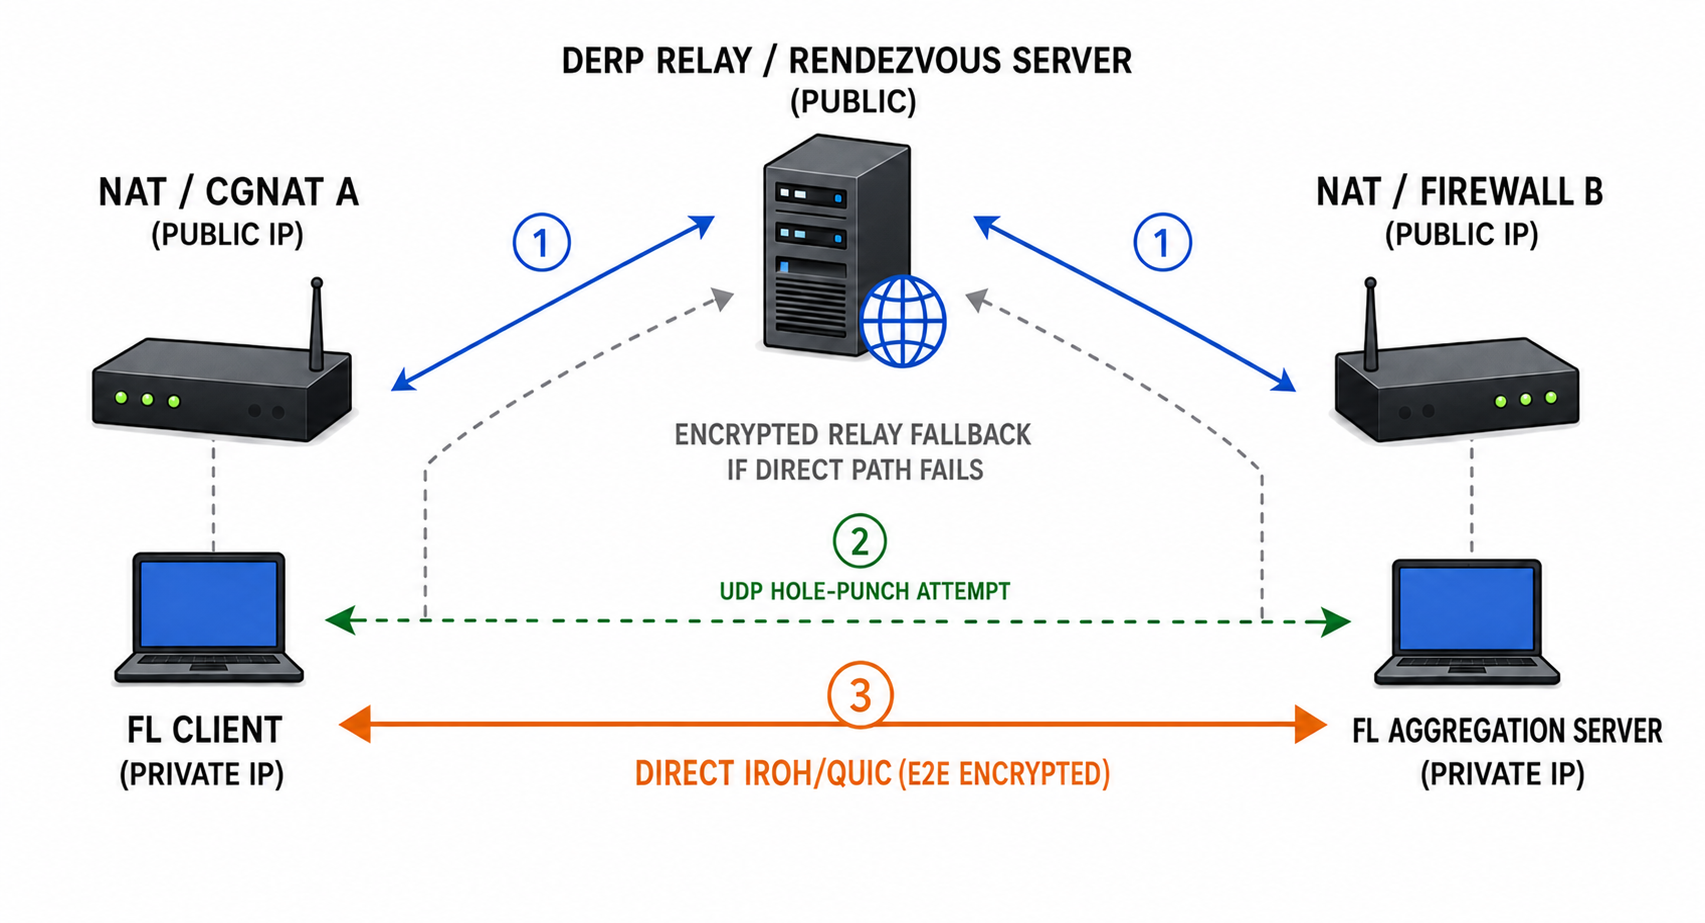
\includegraphics[width=\columnwidth]{NAT-hole-punching.png}
\caption{NAT hole-punching between two peers on private addresses. \textcircled{\scriptsize 1}~Both peers register with a public signaling/rendezvous server through their NATs; \textcircled{\scriptsize 2}~the server relays to each peer the other's public NAT mapping (address:port); \textcircled{\scriptsize 3}~simultaneous outbound packets open pinholes in both NATs and traffic then flows directly between the peers' public endpoints. In FL-Iroh the rendezvous role is played by the DERP relay, which additionally \DIFdelbeginFL \DIFdelFL{serves as an }\DIFdelendFL \DIFaddbeginFL \DIFaddFL{carries the }\DIFaddendFL end-to-end-encrypted \DIFdelbeginFL \DIFdelFL{fallback path }\DIFdelendFL \DIFaddbeginFL \DIFaddFL{traffic }\DIFaddendFL whenever a direct path cannot be \DIFdelbeginFL \DIFdelFL{formed}\DIFdelendFL \DIFaddbeginFL \DIFaddFL{validated}\DIFaddendFL ; \DIFdelbeginFL \DIFdelFL{in our WAN tests the direct path carried 98.3\% of transfers even under CGNAT and a port-443-only firewall, and }\DIFdelendFL the application is unaware of which path is active \DIFaddbeginFL \DIFaddFL{(\S\ref{sec:e3}, \S\ref{sec:e8})}\DIFaddendFL .}
\label{fig:holepunch}
\end{figure}

We address this gap with \textbf{FL-Iroh}, a system that integrates:

\begin{enumerate}
    \item \textbf{Iroh}~\cite{iroh2024}, a QUIC-based P2P transport library that implements the DERP relay protocol~\cite{tailscale2023}: hole-punching is attempted first; \DIFdelbegin \DIFdel{if it fails, all traffic is seamlessly }\DIFdelend \DIFaddbegin \DIFadd{while no direct path is validated, traffic is }\DIFaddend relayed through a DERP server with end-to-end \DIFdelbegin \DIFdel{encryption---the application is unaware of the switchover}\DIFdelend \DIFaddbegin \DIFadd{encryption, and the session migrates to the direct path once it is validated}\DIFaddend .
    \item \textbf{CoAP/CoRE}~\cite{rfc7252} as a lightweight control plane \DIFdelbegin \DIFdel{for FL service discovery (resource directory, round coordination)}\DIFdelend \DIFaddbegin \DIFadd{with an RFC~9176-style resource directory~\mbox{%DIFAUXCMD
\cite{rfc9176} }\hskip0pt%DIFAUXCMD
for capability-based client discovery and round coordination}\DIFaddend , using CBOR serialization \DIFdelbegin \DIFdel{for minimal overhead }\DIFdelend on constrained links\DIFaddbegin \DIFadd{; for peers that are not mutually reachable at the IP level, registration is carried over an authenticated Iroh control stream instead}\DIFaddend .
    \item \textbf{\DIFdelbegin \DIFdel{FedAvg}\DIFdelend \DIFaddbegin \DIFadd{Public-key federation membership}\DIFaddend }\DIFdelbegin \DIFdel{~\mbox{%DIFAUXCMD
\cite{mcmahan2017} }\hskip0pt%DIFAUXCMD
and }\textbf{\DIFdel{FedGAM}} %DIFAUXCMD
\DIFdel{(selective aggregation of the shared seasonality coefficients of Generalized Additive Models, GAMs) as aggregation algorithms, operating over Iroh QUIC streams.
}\DIFdelend \DIFaddbegin \DIFadd{: every node is identified by a persistent Ed25519 key, and the aggregator admits only allow-listed keys at the transport level, before any model exchange.
}\end{enumerate}

\DIFaddend The data plane is independent of IP addressing and \DIFdelbegin \DIFdel{, critically, }\emph{\DIFdel{algorithm-agnostic}}%DIFAUXCMD
\DIFdel{: the same QUIC channel carries neural network weight tensors and Prophet Fourier coefficients without protocol modification.
}%DIFDELCMD < \end{enumerate}
%DIFDELCMD < %%%
\DIFdelend \DIFaddbegin \DIFadd{of the aggregation rule: it carries the serialized parameters of any model without interpreting them, so changing the aggregation (FedAvg, partial aggregation for GAMs, or others) requires no transport change. It is not, however, independent of the client runtime: the current client requires a Python/PyTorch environment on Cortex-A class devices (\S\ref{sec:agnostic}).
}\DIFaddend 

Our primary application domain is agricultural \DIFaddbegin \DIFadd{and environmental }\DIFaddend IoT: soil-based crop recommendation \DIFdelbegin \DIFdel{, where sensors measure N, P, K content, temperature, humidity, pH, and rainfall to recommend optimal crop selection. This represents a tabular inference task well-suited for lightweight MLP models on Cortex-A class edge devices (e.g., }\DIFdelend \DIFaddbegin \DIFadd{and seven-day-ahead outdoor air-quality forecasting with lightweight models suited to single-board edge computers such as the }\DIFaddend Raspberry Pi~\DIFdelbegin \DIFdel{4B), with potential for inference deployment on more constrained platforms}\DIFdelend \DIFaddbegin \DIFadd{3B used in our hardware experiments}\DIFaddend .

\noindent\textbf{Contributions:}
\begin{enumerate}
    \item We design and implement FL-Iroh, an open-source \DIFdelbegin \DIFdel{, algorithm-agnostic }\DIFdelend FL architecture that embeds NAT traversal in the application-level transport---an Iroh\slash QUIC data plane with public-key \DIFdelbegin \DIFdel{peer addressing---coordinated by a lightweight }\DIFdelend \DIFaddbegin \DIFadd{addressing, transport-level admission control, transfer retry and endpoint recovery---coordinated by a }\DIFaddend CoAP\slash CBOR control plane \DIFaddbegin \DIFadd{with a resource directory }\DIFaddend (\S\ref{sec:system}). The NAT-traversal machinery \DIFdelbegin \DIFdel{itself }\DIFdelend is provided by the Iroh library~\cite{iroh2024}; our contribution is its integration into, \DIFaddbegin \DIFadd{hardening for, }\DIFaddend and evaluation as \DIFdelbegin \DIFdel{, }\DIFdelend an FL substrate.
    \item We provide an empirical \DIFdelbegin \DIFdel{characterization of QUIC hole-punching and relay transport for FL workloads }\DIFdelend \DIFaddbegin \DIFadd{connectivity characterization }\DIFaddend on real hardware \DIFdelbegin \DIFdel{(PC $\leftrightarrow$ Raspberry Pi across a 300~km WAN, different ISPs): every session in the transfer campaign connected, 118 of 120 WAN transfers (98.3\%) used a direct hole-punched path---verified by active-path inspection---and a repeated }\DIFdelend \DIFaddbegin \DIFadd{across five networks with RFC~4787-classified NAT behavior---including a mobile-carrier CGNAT---covering }\DIFaddend cold-start \DIFdelbegin \DIFdel{campaign established a direct path on 145 of 150 attempts (96.7\%, 0\% relay ), under full-cone NAT, symmetric NAT, CGNAT, and a port-443-only firewall, with the encrypted relay retained as a guaranteed fallback }\DIFdelend \DIFaddbegin \DIFadd{establishment, path validation in long-lived sessions, forced relay operation, link outages and network switches }\DIFaddend (\S\ref{sec:e3}\DIFaddbegin \DIFadd{, \S\ref{sec:e8}). We distinguish validated direct paths from relay-carried ones, a distinction that our earlier analysis had conflated.
    }\item \DIFadd{We evaluate FL-Iroh end to end: convergence and churn (E2, E4}\DIFaddend )\DIFdelbegin \DIFdel{.
    }%DIFDELCMD < \item %%%
\item%DIFAUXCMD
\DIFdel{We conduct a six-experiment evaluation (E1--E6) plus an operational comparison with Flower-over-Tailscale, covering transport throughput, convergence under Non-IID heterogeneity, churn resilience}\DIFdelend , CoAP discovery scaling \DIFaddbegin \DIFadd{to 5}{\DIFaddend ,\DIFdelbegin \DIFdel{and }\DIFdelend \DIFaddbegin }\DIFadd{000 endpoints (E5), }\DIFaddend a two-domain application study \DIFdelbegin \DIFdel{: crop recommendation with a compact MLP (AgriMLP, 7.7K parameters)and seven-day-ahead air-quality forecasting (\S\ref{sec:evaluation}).
}%DIFDELCMD < \item %%%
\item%DIFAUXCMD
\DIFdel{We propose FedGAM, }\DIFdelend \DIFaddbegin \DIFadd{with imbalance-aware metrics (E6), a packet-loss/latency/bandwidth sweep (E9), admission control (E10), and a complete federation over the WAN with a Raspberry Pi~3B client, including per-round CPU, memory and energy (E11).
}\end{enumerate}

\DIFadd{We also include a case study of }\DIFaddend a partial-aggregation rule \DIFdelbegin \DIFdel{that federates only the shared seasonality coefficients of Prophet GAM models, and report an honest }\DIFdelend \DIFaddbegin \DIFadd{for Prophet GAMs (FedGAM). A }\DIFaddend same-model ablation \DIFdelbegin \DIFdel{showing that , with eight years of local training data, FedGAM }\DIFdelend \DIFaddbegin \DIFadd{shows that it }\DIFaddend is statistically indistinguishable from \DIFdelbegin \DIFdel{FedAvg---delimiting the regime in which partial aggregation can matter }\DIFdelend \DIFaddbegin \DIFadd{FedAvg on our data, so we present it as an illustration of aggregation-agnostic transport rather than as a contribution in its own right }\DIFaddend (\S\ref{sec:e6}).
\DIFdelbegin %DIFDELCMD < \end{enumerate}
%DIFDELCMD < %%%
\DIFdelend 

The remainder of this paper is organized as follows. Section~\ref{sec:related} reviews related work. Section~\ref{sec:system} presents the FL-Iroh architecture \DIFdelbegin \DIFdel{, transport, control plane, and application models}\DIFdelend \DIFaddbegin \DIFadd{and protocols}\DIFaddend . Section~\ref{sec:evaluation} reports the experimental evaluation\DIFdelbegin \DIFdel{(E1--E6) and the operational comparison with Flower-over-Tailscale}\DIFdelend . Section~\ref{sec:discussion} discusses implications, the security model, and limitations. Section~\ref{sec:conclusion} concludes and outlines \DIFdelbegin \DIFdel{future work}\DIFdelend \DIFaddbegin \DIFadd{a research roadmap}\DIFaddend .

% =========================================================================
\section{Related Work}
\label{sec:related}

We organize prior work along \DIFdelbegin \DIFdel{five axes: FL }\DIFdelend \DIFaddbegin \DIFadd{six axes---FL }\DIFaddend in agriculture and environmental monitoring, \DIFaddbegin \DIFadd{communication-efficient and resource-aware FL, }\DIFaddend NAT traversal, \DIFdelbegin \DIFdel{control planes for IoT ML, Non-IID mitigation, and alternative connectivity substrates (overlay VPNs and decentralized FL}\DIFdelend \DIFaddbegin \DIFadd{lightweight IoT protocols for FL, FL over overlays, and decentralized FL---and close with a structured comparison (Table~\ref{tab:related}}\DIFaddend ).

\subsection{Federated Learning for Agricultural and Environmental IoT}

FL has \DIFdelbegin \DIFdel{recently }\DIFdelend been applied across the agri-food sector\DIFdelbegin \DIFdel{. Durrant~et~al.~\mbox{%DIFAUXCMD
\cite{durrant2022} }\hskip0pt%DIFAUXCMD
demonstrate }\DIFdelend \DIFaddbegin \DIFadd{, from }\DIFaddend cross-silo \DIFdelbegin \DIFdel{FL for collaborative }\DIFdelend data sharing among \DIFdelbegin \DIFdel{agricultural stakeholders, and Friha~et~al.~\mbox{%DIFAUXCMD
\cite{friha2022} }\hskip0pt%DIFAUXCMD
propose a federated intrusion-detection system (FELIDS) for the agricultural Internet of Things. Device heterogeneity across farms---different soil types, crops, and microclimates---creates natural Non-IID distributions that challenge standard FedAvg~\mbox{%DIFAUXCMD
\cite{mcmahan2017}}\hskip0pt%DIFAUXCMD
. Privacy is also a first-order concern: agronomic data (crop varieties, yields, fertilization schedules) }\DIFdelend \DIFaddbegin \DIFadd{stakeholders~\mbox{%DIFAUXCMD
\cite{durrant2022} }\hskip0pt%DIFAUXCMD
and federated intrusion detection for agricultural IoT~\mbox{%DIFAUXCMD
\cite{friha2022} }\hskip0pt%DIFAUXCMD
to crop-yield prediction with encrypted gradients in an edge--cloud hierarchy~\mbox{%DIFAUXCMD
\cite{dey2025}}\hskip0pt%DIFAUXCMD
, nitrous-oxide emission prediction on a farm-deployed IoT/fog architecture~\mbox{%DIFAUXCMD
\cite{killeen2025}}\hskip0pt%DIFAUXCMD
, and leaf-disease detection with pruned attention networks~\mbox{%DIFAUXCMD
\cite{piccialli2025}}\hskip0pt%DIFAUXCMD
. In environmental monitoring, federated models forecast PM2.5 across city-level edge servers~\mbox{%DIFAUXCMD
\cite{hu2024} }\hskip0pt%DIFAUXCMD
and air-quality indices with energy-aware training~\mbox{%DIFAUXCMD
\cite{dey2026}}\hskip0pt%DIFAUXCMD
, and detect anomalies in environmental sensor networks~\mbox{%DIFAUXCMD
\cite{yan2024}}\hskip0pt%DIFAUXCMD
. Geographic heterogeneity creates natural non-IID distributions, and agronomic data }\DIFaddend are commercially sensitive\DIFdelbegin \DIFdel{and farmers are reluctant to share them. However, }\DIFdelend \DIFaddbegin \DIFadd{. All }\DIFaddend these works assume \DIFdelbegin \DIFdel{publicly reachable aggregation servers reached }\DIFdelend \DIFaddbegin \DIFadd{that clients can reach an aggregator }\DIFaddend over conventional infrastructure (\DIFdelbegin \DIFdel{cross-silo data centersor }\DIFdelend \DIFaddbegin \DIFadd{data centers, }\DIFaddend pre-provisioned gateways \DIFaddbegin \DIFadd{or a single-site network}\DIFaddend ); none addresses the NAT-traversal barrier that \DIFdelbegin \DIFdel{, in our experience, is a major practical obstacle to real-world agricultural FLdeployment in rural environments with NAT}\DIFdelend \DIFaddbegin \DIFadd{rural deployments behind NAT}\DIFaddend /\DIFdelbegin \DIFdel{CGNAT. FL applications to outdoor air-quality monitoring---our second domain---remain scarce in the literature}\DIFdelend \DIFaddbegin \DIFadd{CGNAT face.
}

\subsection{\DIFadd{Communication-Efficient and Resource-Aware FL at the Edge}}

\DIFadd{A large body of work reduces what FL sends: quantization and sparsification with error feedback~\mbox{%DIFAUXCMD
\cite{konecny2016,malik2026}}\hskip0pt%DIFAUXCMD
, compressed and pruned updates with energy- and latency-aware synchronization for intermittent edge--cloud participants~\mbox{%DIFAUXCMD
\cite{bayraktar2026}}\hskip0pt%DIFAUXCMD
, and joint analyses of communication efficiency and energy footprint for robust FL in industrial IoT~\mbox{%DIFAUXCMD
\cite{barbieri2025}}\hskip0pt%DIFAUXCMD
. Resource use on real edge hardware has been measured on Raspberry Pi testbeds~\mbox{%DIFAUXCMD
\cite{ridolfi2023}}\hskip0pt%DIFAUXCMD
, embedded intrusion-detection deployments~\mbox{%DIFAUXCMD
\cite{bhavsar2024} }\hskip0pt%DIFAUXCMD
and energy-aware benchmarks under emulated device constraints~\mbox{%DIFAUXCMD
\cite{miller2026}}\hskip0pt%DIFAUXCMD
. These approaches are complementary to ours: they reduce payloads or schedule participation, but assume a reachable server; FL-Iroh addresses reachability and transport, and could carry their compressed updates unchanged.
}

\subsection{\DIFadd{Non-IID Data in Resource-Constrained Federations}}

\DIFadd{Non-IID data is a well-studied challenge in FL~\mbox{%DIFAUXCMD
\cite{zhao2018noniid,li2022noniid,kairouz2021}}\hskip0pt%DIFAUXCMD
; in agriculture it arises naturally from climate zones and soil types. FedProx~\mbox{%DIFAUXCMD
\cite{fedprox2020} }\hskip0pt%DIFAUXCMD
and SCAFFOLD~\mbox{%DIFAUXCMD
\cite{scaffold2020} }\hskip0pt%DIFAUXCMD
counter client drift, and clustering approaches group clients with similar distributions~\mbox{%DIFAUXCMD
\cite{briggs2020cluster}}\hskip0pt%DIFAUXCMD
. For non-neural models such as Prophet GAMs, plain FedAvg averages parameters whose meaning differs across clients (e.g., local emission trends)}\DIFaddend , which motivates the \DIFdelbegin \DIFdel{E6 study in this paper}\DIFdelend \DIFaddbegin \DIFadd{partial-aggregation case study of \S\ref{sec:e6}. We use Dirichlet partitions as the standard non-IID benchmark in E2 and E4}\DIFaddend .

\subsection{NAT Traversal in P2P and IoT}

NAT traversal has been studied \DIFdelbegin \DIFdel{extensively }\DIFdelend since Ford et~al.'s \DIFdelbegin \DIFdel{foundational }\DIFdelend analysis of peer-to-peer communication across NATs~\cite{ford2005,rfc5128}, and underpins VoIP, WebRTC~\cite{webrtc2021} \DIFdelbegin \DIFdel{, and file-sharing systems. The }\DIFdelend \DIFaddbegin \DIFadd{and file sharing. RFC~4787~\mbox{%DIFAUXCMD
\cite{rfc4787} }\hskip0pt%DIFAUXCMD
defines the NAT mapping and filtering behaviors that determine hole-punching success; }\DIFaddend STUN~\cite{rfc8489} and TURN~\cite{rfc8656} \DIFdelbegin \DIFdel{protocols provide the IETF foundations for hole-punching and relay fallback, and large-scale }\DIFdelend \DIFaddbegin \DIFadd{provide the corresponding discovery and relay protocols, and }\DIFaddend measurement campaigns in the libp2p ecosystem have characterized hole-punching success \DIFdelbegin \DIFdel{rates }\DIFdelend in the wild~\cite{seemann2022}. DERP\DIFdelbegin \DIFdel{(Designated Encrypted Relay for Packets)}\DIFdelend , developed by Tailscale~\cite{tailscale2023}, \DIFdelbegin \DIFdel{provides }\DIFdelend \DIFaddbegin \DIFadd{is }\DIFaddend an authenticated, encrypted, HTTPS-based relay that acts both as \DIFdelbegin \DIFdel{a rendezvous /signaling channel and as a }\DIFdelend \DIFaddbegin \DIFadd{rendezvous and as }\DIFaddend relay of last \DIFdelbegin \DIFdel{resort---fulfilling the same architectural role as TURN, though it is not protocol-compatible with it---within the WireGuard VPN ecosystem. Iroh adapts DERP }\DIFdelend \DIFaddbegin \DIFadd{resort---the role of TURN, without protocol compatibility---and Iroh adapts it }\DIFaddend for general-purpose P2P applications~\cite{iroh2024}. \DIFdelbegin \DIFdel{In the IoT space, NGROK and similar tunneling services provide connectivity but introduce centralized dependencies and per-byte costs unsuitable for energy-constrained deployments}\DIFdelend \DIFaddbegin \DIFadd{The most closely related FL study compares communication substrates (gRPC, MQTT, DDS and QUIC) for distributed learning under emulated disruption~\mbox{%DIFAUXCMD
\cite{kutlu2026}}\hskip0pt%DIFAUXCMD
; it treats QUIC as a client--server transport and does not consider NAT traversal, peer addressing or discovery}\DIFaddend .

\subsection{\DIFdelbegin \DIFdel{CoAP }\DIFdelend \DIFaddbegin \DIFadd{Lightweight IoT Protocols }\DIFaddend for FL Control \DIFdelbegin \DIFdel{Plane}\DIFdelend \DIFaddbegin \DIFadd{and Transport}\DIFaddend }

CoAP~\cite{rfc7252}\DIFdelbegin \DIFdel{(Constrained Application Protocol) provides a RESTful transfer protocol for constrained nodes and, together with }\DIFdelend \DIFaddbegin \DIFadd{, }\DIFaddend the CoRE link format~\cite{rfc6690}\DIFaddbegin \DIFadd{, the CoRE resource directory~\mbox{%DIFAUXCMD
\cite{rfc9176} }\hskip0pt%DIFAUXCMD
}\DIFaddend and CBOR~\cite{rfc8949} \DIFdelbegin \DIFdel{(Concise Binary Object Representation) encoding, is a natural candidate for a lightweight }\emph{\DIFdel{control plane}} %DIFAUXCMD
\DIFdel{for IoT ML pipelines, separating signaling (discovery, round coordination) from bulk data transfer. MQTT~\mbox{%DIFAUXCMD
\cite{mqtt2019}}\hskip0pt%DIFAUXCMD
-based publish--subscribe signaling has also been used to coordinate distributed and federated training in IoT deployments; MQTT, however, lacks the RESTful resource model that enables semantic client filtering by sensor capability. To the best of our knowledge, no prior FL system combines a CoAP control plane with a NAT-traversing data-plane transport; CoAP-coordinated FL itself remains largely unevaluated. Our work uses CoAP exclusively as the control plane (registration, discovery, round signaling); model parameter transfer---the }\emph{\DIFdel{data plane}}%DIFAUXCMD
\DIFdel{---occurs over Iroh/QUIC, which handles NAT traversal transparently and independently from the control channel.
}%DIFDELCMD < 

%DIFDELCMD < %%%
\subsection{\DIFdel{Non-IID FL in Resource-Constrained Environments}}
%DIFAUXCMD
\addtocounter{subsection}{-1}%DIFAUXCMD
%DIFDELCMD < 

%DIFDELCMD < %%%
\DIFdel{Non-IID data is a well-studied challenge in FL~\mbox{%DIFAUXCMD
\cite{zhao2018noniid,li2022noniid,kairouz2021}}\hskip0pt%DIFAUXCMD
. In agricultural settings, non-IID arises naturally from geographic heterogeneity: farms in different climate zones or with different soil types exhibit clearly distinct feature distributions. FedProx~\mbox{%DIFAUXCMD
\cite{fedprox2020} }\hskip0pt%DIFAUXCMD
and SCAFFOLD~\mbox{%DIFAUXCMD
\cite{scaffold2020} }\hskip0pt%DIFAUXCMD
mitigate gradient drift by regularizing against deviation from the global model, and client-clustering approaches group clients with similar local distributions before aggregation~\mbox{%DIFAUXCMD
\cite{briggs2020cluster}}\hskip0pt%DIFAUXCMD
. For non-neural models---such as Prophet GAMs---plain FedAvg is semantically questionable: it averages parameters whose local meanings differ across clients (e.g. , the industrial emission trend of Ponferrada with the rural baseline of Soria)}\DIFdelend \DIFaddbegin \DIFadd{form the standard stack for constrained RESTful environments. FedCoRE carries federated training over CoAP with quantized models on microcontroller-class devices~\mbox{%DIFAUXCMD
\cite{djamaa2025}}\hskip0pt%DIFAUXCMD
, and TDMiL uses a CoAP-based aggregator for distributed training on microcontrollers~\mbox{%DIFAUXCMD
\cite{gulati2024}}\hskip0pt%DIFAUXCMD
; MQTT~\mbox{%DIFAUXCMD
\cite{mqtt2019} }\hskip0pt%DIFAUXCMD
and brokered protocols such as Zenoh have been compared for resilient edge FL~\mbox{%DIFAUXCMD
\cite{almeida2025}}\hskip0pt%DIFAUXCMD
. These systems use the IoT protocol as the }\emph{\DIFadd{data}} \DIFadd{transport inside a local network}\DIFaddend . FL-Iroh \DIFdelbegin \DIFdel{explores FedGAM, which applies }\emph{\DIFdel{partial aggregation}} %DIFAUXCMD
\DIFdel{over the shared seasonality coefficients only; our evaluation both demonstrates this design and , via a same-model ablation, delimits when it actually pays off (\S\ref{sec:e6}). We use Dirichlet $\alpha$ partitions as the standard Non-IID benchmark in E2}\DIFdelend \DIFaddbegin \DIFadd{instead uses CoAP and a resource directory as a }\emph{\DIFadd{control}} \DIFadd{plane for capability-based discovery and moves bulk transfers to a NAT-traversing QUIC data plane, so that the two compose across the Internet}\DIFaddend .

\subsection{FL over Overlay and VPN Networks}

A pragmatic way to reach NATed devices is \DIFdelbegin \DIFdel{to place them on }\DIFdelend a shared overlay network. WireGuard~\cite{wireguard2017}-based meshes such as Tailscale~\cite{tailscale2023} and ZeroTier give every node a stable virtual IP and traverse NAT/CGNAT \DIFdelbegin \DIFdel{through the same }\DIFdelend \DIFaddbegin \DIFadd{with }\DIFaddend DERP-style relays\DIFdelbegin \DIFdel{that Iroh uses, and have been adopted to interconnect distributed-ML and edge clusters. Relative to FL-Iroh, however, these approaches }\DIFdelend \DIFaddbegin \DIFadd{. They }\DIFaddend delegate connectivity to a \DIFdelbegin \DIFdel{separate }\DIFdelend system-level \DIFdelbegin \DIFdel{VPN daemon---typically requiring }\DIFdelend \DIFaddbegin \DIFadd{daemon with }\DIFaddend elevated privileges and an account-managed coordination \DIFdelbegin \DIFdel{server---while }\DIFdelend \DIFaddbegin \DIFadd{server, while }\DIFaddend the FL framework \DIFdelbegin \DIFdel{itself }\DIFdelend (e.g., Flower~\cite{flower2022}) \DIFdelbegin \DIFdel{must still address a reachable server over a centralized star topology}\DIFdelend \DIFaddbegin \DIFadd{still addresses a reachable star-topology server}\DIFaddend . FL-Iroh \DIFdelbegin \DIFdel{instead embeds NAT }\DIFdelend \DIFaddbegin \DIFadd{embeds }\DIFaddend traversal in the \DIFdelbegin \DIFdel{application-level transport : peers are named }\DIFdelend \DIFaddbegin \DIFadd{application transport and names peers }\DIFaddend by public key \DIFdelbegin \DIFdel{rather than by overlay IP, and no system VPN or persistent server address is required. We provide a qualitative operational comparison against Flower-over-Tailscale, together with an accuracy-parity check using a Flower-compatible harness, in \S\ref{sec:e7}}\DIFdelend \DIFaddbegin \DIFadd{(\S\ref{sec:flower})}\DIFaddend .

\subsection{Decentralized and Serverless FL}

\DIFdelbegin \DIFdel{An orthogonal line of work removes the central aggregator altogether. }\DIFdelend Decentralized SGD trains over sparse \DIFdelbegin \DIFdel{communication }\DIFdelend graphs without a parameter server~\cite{lian2017}, gossip learning \DIFdelbegin \DIFdel{propagates and }\DIFdelend merges models epidemically\DIFdelbegin \DIFdel{among peers}\DIFdelend ~\cite{hegedus2019}, \DIFdelbegin \DIFdel{and BrainTorrent demonstrates }\DIFdelend \DIFaddbegin \DIFadd{including over opportunistic contacts among mobile users~\mbox{%DIFAUXCMD
\cite{rizzo2026}}\hskip0pt%DIFAUXCMD
, BrainTorrent performs }\DIFaddend peer-to-peer FL \DIFdelbegin \DIFdel{without a central server }\DIFdelend in medical imaging~\cite{roy2019braintorrent}\DIFdelbegin \DIFdel{. These approaches address the aggregator as a statistical and topological bottleneck, but generally }\emph{\DIFdel{assume}} %DIFAUXCMD
\DIFdel{that peers can reach one another---precisely the assumption that NAT and CGNAT break in the field. Production-oriented FL }\DIFdelend \DIFaddbegin \DIFadd{, and Fedstellar supports centralized, semi-decentralized and decentralized topologies on physical devices~\mbox{%DIFAUXCMD
\cite{martinezbeltran2024}}\hskip0pt%DIFAUXCMD
. Production }\DIFaddend frameworks (Flower~\cite{flower2022}, FedML~\cite{fedml2020}, OpenFL~\cite{openfl2022}, NVIDIA FLARE~\cite{flare2022}) likewise assume a reachable coordination endpoint. \DIFaddbegin \DIFadd{These approaches generally }\emph{\DIFadd{assume}} \DIFadd{that peers can address one another---the assumption NAT and CGNAT break in the field. Decentralized networking among resource-constrained edge platforms has also been explored outside FL, e.g., congestion-aware mesh routing in UAV swarms~\mbox{%DIFAUXCMD
\cite{bakirci2023}}\hskip0pt%DIFAUXCMD
. }\DIFaddend FL-Iroh is complementary: it \DIFdelbegin \DIFdel{retains }\DIFdelend \DIFaddbegin \DIFadd{keeps }\DIFaddend a logical aggregator \DIFdelbegin \DIFdel{(simplifying convergence semantics) }\DIFdelend while removing the requirement that any participant be publicly routable\DIFdelbegin \DIFdel{; }\DIFdelend \DIFaddbegin \DIFadd{, and }\DIFaddend because peers are addressed by public key \DIFdelbegin \DIFdel{, }\DIFdelend the same transport could \DIFdelbegin \DIFdel{also carry the fully }\DIFdelend \DIFaddbegin \DIFadd{carry the }\DIFaddend decentralized topologies above.

\DIFaddbegin \subsection{\DIFadd{Comparison and Research Gap}}

\DIFadd{Table~\ref{tab:related} compares representative recent works on the problem addressed, the key innovation, the methodology and evaluation, the main reported result, and the gap that remains with respect to the requirements of rural IoT FL. Three gaps recur: (i)~reachability of the aggregator (or of peers) is assumed rather than provided; (ii)~connectivity is evaluated in simulation or on a single local network rather than across real NATs and mobile carriers; and (iii)~discovery and federation membership are not part of the system. FL-Iroh (last row) targets all three, at the cost of a heavier client runtime than the microcontroller-oriented CoAP systems.
}

\begin{table*}[!t]
\centering
\caption{\DIFaddFL{Comparison of recent related work (2023--2026) with FL-Iroh}}
\label{tab:related}
\scriptsize
\renewcommand{\arraystretch}{1.15}
\setlength{\tabcolsep}{3pt}
\begin{tabular}{@{}p{1.75cm} p{2.6cm} p{3.0cm} p{2.9cm} p{2.6cm} p{3.6cm}@{}}
\toprule
\textbf{Work} & \textbf{Problem} & \textbf{Innovation} & \textbf{Methodology} & \textbf{Main result} & \textbf{Gap w.r.t.\ NAT-constrained IoT FL} \\
\midrule
FLyer~\cite{dey2025} & Private crop-yield prediction & Edge--cloud FL with LSTM and AES-encrypted gradients & Edge servers + cloud aggregator & $\approx$39\% lower latency, $\approx$40\% lower energy & Assumes reachable cloud; no NAT, discovery or WAN tests \\
Killeen et~al.~\cite{killeen2025} & Smart-farming adoption barriers & IoT/fog FL architecture replacing N$_2$O sensors & Prototype on a farm; centralized vs.\ federated & FL competitive with centralized & Connectivity and NAT not studied \\
AGRIFOLD~\cite{piccialli2025} & Leaf-disease detection & Pruned attention CNN for edge devices & Five FL algorithms on 12 datasets (simulation) & SCAFFOLD best & No networking evaluation \\
FedDeep~\cite{hu2024} & Multi-city PM2.5 forecasting & Spatio-temporal network per edge cloud & 13 cities, edge servers & Outperforms baselines & Data-center edge; no constrained devices or NAT \\
GreenEdge AI~\cite{dey2026} & Energy-efficient AQI forecasting & Green-aware LSTM and aggregation & Edge FL with energy metrics & 37\% lower compute cost & Reachable aggregator assumed \\
Barbieri et~al.~\cite{barbieri2025} & Energy/carbon cost of IIoT FL & Energy and GHG monitoring incl.\ compression & Case studies, centralized and decentralized FL & Centralized FL best under tight budgets & Communication modeled; no transport/NAT \\
Bayraktar \& Bakirci~\cite{bayraktar2026} & Bandwidth-limited edge--cloud FL & Quantized, pruned deltas; energy-aware sync & UAV/industrial vision, non-IID sites & $>$50\% less communication & Star topology with reachable cloud; no NAT \\
Ridolfi et~al.~\cite{ridolfi2023} & FL on heterogeneous devices & Flower testbed of Raspberry Pis and VMs & Image classification on LAN & Effects of heterogeneity and heat & LAN only; reachable server \\
EcoFL~\cite{miller2026} & System-level FL resource use & Energy-aware scheduler and profiling & Emulated RPi~4 constraints & Reproducible energy profiles & Emulated devices; no real network \\
Kutlu~\cite{kutlu2026} & Transport choice for distributed ML & Controlled DDS/gRPC/MQTT/QUIC comparison & Physical testbed, netem disruptions & gRPC 96$\to$55\% efficiency at 20\% loss & No NAT traversal, peer addressing or discovery \\
Almeida et~al.~\cite{almeida2025} & Resilient FL at a dynamic edge & Pluggable protocols (Zenoh/MQTT/Kafka) & Simulated worker failures & Zenoh most efficient & Brokered/routed; no NAT \\
Fedstellar~\cite{martinezbeltran2024} & Platform for decentralized FL & Configurable topologies, live monitoring & Raspberry Pi deployment + virtual nodes & F1 up to 98\% & Nodes assumed addressable \\
FedCoRE~\cite{djamaa2025} & FL on MCU-class AIoT & FL over CoAP with quantization & 256~KB-RAM devices & Up to 60\% less communication & Local network; no NAT/P2P \\
TDMiL~\cite{gulati2024} & Tiny distributed ML on MCUs & CoAP aggregator + embedded runtimes & COTS boards, open testbed & Straggler mitigation compared & Single site; no WAN \\
\midrule
\textbf{FL-Iroh (this work)} & FL across NAT/CGNAT without public IPs & QUIC P2P data plane with public-key addressing, admission control and relay fallback; CoAP RD control plane & Real hardware across 5 RFC~4787-classified networks incl.\ mobile CGNAT; WAN federation on RPi~3B; netem sweep; 5{,}000-endpoint discovery & Connectivity in all new sessions; relay 190/190 without UDP; 29/30 WAN rounds; 19~ms RD lookup at 5{,}000 & Python/PyTorch runtime too heavy for MCUs; small physical federation; cold starts often relay-carried \\
\bottomrule
\end{tabular}
\end{table*}

\DIFaddend % =========================================================================
\section{System Design}
\label{sec:system}

This section describes the FL-Iroh architecture (control and data planes), \DIFaddbegin \DIFadd{node identity and admission control, }\DIFaddend the Iroh transport and \DIFaddbegin \DIFadd{its hardening, the }\DIFaddend wire format, the CoAP control plane \DIFaddbegin \DIFadd{and resource directory, the round protocol}\DIFaddend , and the application models used in the evaluation. Fig.~\ref{fig:agro} illustrates the target deployment: field sensors feed a \DIFdelbegin \DIFdel{Raspberry-Pi-class }\DIFdelend \DIFaddbegin \DIFadd{single-board }\DIFaddend FL client that registers \DIFdelbegin \DIFdel{via CoAP }\DIFdelend \DIFaddbegin \DIFadd{with the aggregator }\DIFaddend and exchanges model parameters over Iroh/QUIC from behind NAT or CGNAT.

\subsection{Architecture Overview}

FL-Iroh is structured as two planes (Fig.~\ref{fig:architecture}) \DIFdelbegin \DIFdel{:
}\DIFdelend \DIFaddbegin \DIFadd{and four software components that run unchanged on the aggregator and on every client (Table~\ref{tab:components}).
}\DIFaddend 

\begin{itemize}
    \item \DIFdelbegin \textbf{\DIFdel{Control plane (CoAP/CoRE)}}%DIFAUXCMD
\DIFdel{: A CoAP resource directory running on the FL aggregation node. Clients register their Iroh endpoint descriptors (node ID, addresses, relay URL)as CoAP resources on startup.
The server discovers clients, manages round state, and disseminates lightweight round metadata (}\texttt{\DIFdel{round\_id}}%DIFAUXCMD
\DIFdel{, }\texttt{\DIFdel{model\_hash}}%DIFAUXCMD
\DIFdel{, server node ID) via CoAPGET/PUT with CBOR encoding; clients then fetch the model tensors over Iroh}\DIFdelend \DIFaddbegin \textbf{\DIFadd{Control plane}}\DIFadd{: registration, discovery and round signaling. Within a site (farm LAN, cooperative network) it uses CoAP}\DIFaddend /\DIFdelbegin \DIFdel{QUIC (Application-Layer Protocol Negotiation, ALPN , identifier }\DIFdelend \DIFaddbegin \DIFadd{CoRE with CBOR payloads and a resource directory (\S\ref{sec:coap}). Across NATs, where the aggregator's CoAP port is not reachable, the same registration message is carried over an Iroh stream (ALPN }\DIFaddend \texttt{\DIFdelbegin \DIFdel{fl-model}\DIFdelend \DIFaddbegin \DIFadd{fl-ctrl}\DIFaddend /1}) \DIFaddbegin \DIFadd{addressed only by the aggregator's public key, so the control plane traverses NAT exactly like the data plane}\DIFaddend .
    \item \textbf{Data plane (Iroh/QUIC)}: \DIFdelbegin \DIFdel{All tensor data---model distributions }\DIFdelend \DIFaddbegin \DIFadd{all tensor data---global model distribution }\DIFaddend (server$\to$client\DIFdelbegin \DIFdel{) and gradient uploads }\DIFdelend \DIFaddbegin \DIFadd{, ALPN }\texttt{\DIFadd{fl-model/1}}\DIFadd{) and local updates }\DIFaddend (client$\to$server\DIFdelbegin \DIFdel{)---flow }\DIFdelend \DIFaddbegin \DIFadd{, ALPN }\texttt{\DIFadd{fl-update/1}}\DIFadd{)---flows }\DIFaddend over QUIC streams established by Iroh. Each \DIFdelbegin \DIFdel{QUIC stream carries a }\DIFdelend \DIFaddbegin \DIFadd{stream carries one }\DIFaddend length-prefixed, SHA-256-verified payload \DIFdelbegin \DIFdel{. The ALPN protocol identifiers }\texttt{\DIFdel{fl-model/1}} %DIFAUXCMD
\DIFdel{and }\texttt{\DIFdel{fl-update/1}} %DIFAUXCMD
\DIFdel{distinguish model push from update upload}\DIFdelend \DIFaddbegin \DIFadd{(\S\ref{sec:wire})}\DIFaddend .
\end{itemize}

\DIFaddbegin \begin{table}[t]
\centering
\caption{\DIFaddFL{FL-Iroh software components (Python package }\texttt{\DIFaddFL{fl\_coap\_iroh}}\DIFaddFL{)}}
\label{tab:components}
\scriptsize
\setlength{\tabcolsep}{3pt}
\begin{tabular}{@{}p{2.0cm} p{5.9cm}@{}}
\toprule
\textbf{Component} & \textbf{Responsibility} \\
\midrule
Transport node & Iroh endpoint with persistent Ed25519 key; per-ALPN accept queues; admission check; framed send/receive with integrity check, transfer retry and endpoint watchdog; path classification (direct / mixed / relay). \\
Admission & Allow-list of authorized node IDs; rejection log; persistent key management (\texttt{fl-keygen}). \\
CoAP server & Resources \texttt{/fl/*}, \texttt{/iroh/endpoint}, \texttt{/fl/register}; resource directory \texttt{/rd}, \texttt{/rd-lookup/ep} on the aggregator. \\
FL server / client & Round orchestration, aggregation (pluggable \texttt{aggregator\_fn}), local training, per-round metrics and resource monitoring (CPU, RSS, power/energy). \\
\bottomrule
\end{tabular}
\end{table}

\DIFaddend \begin{figure}[t]
\centering
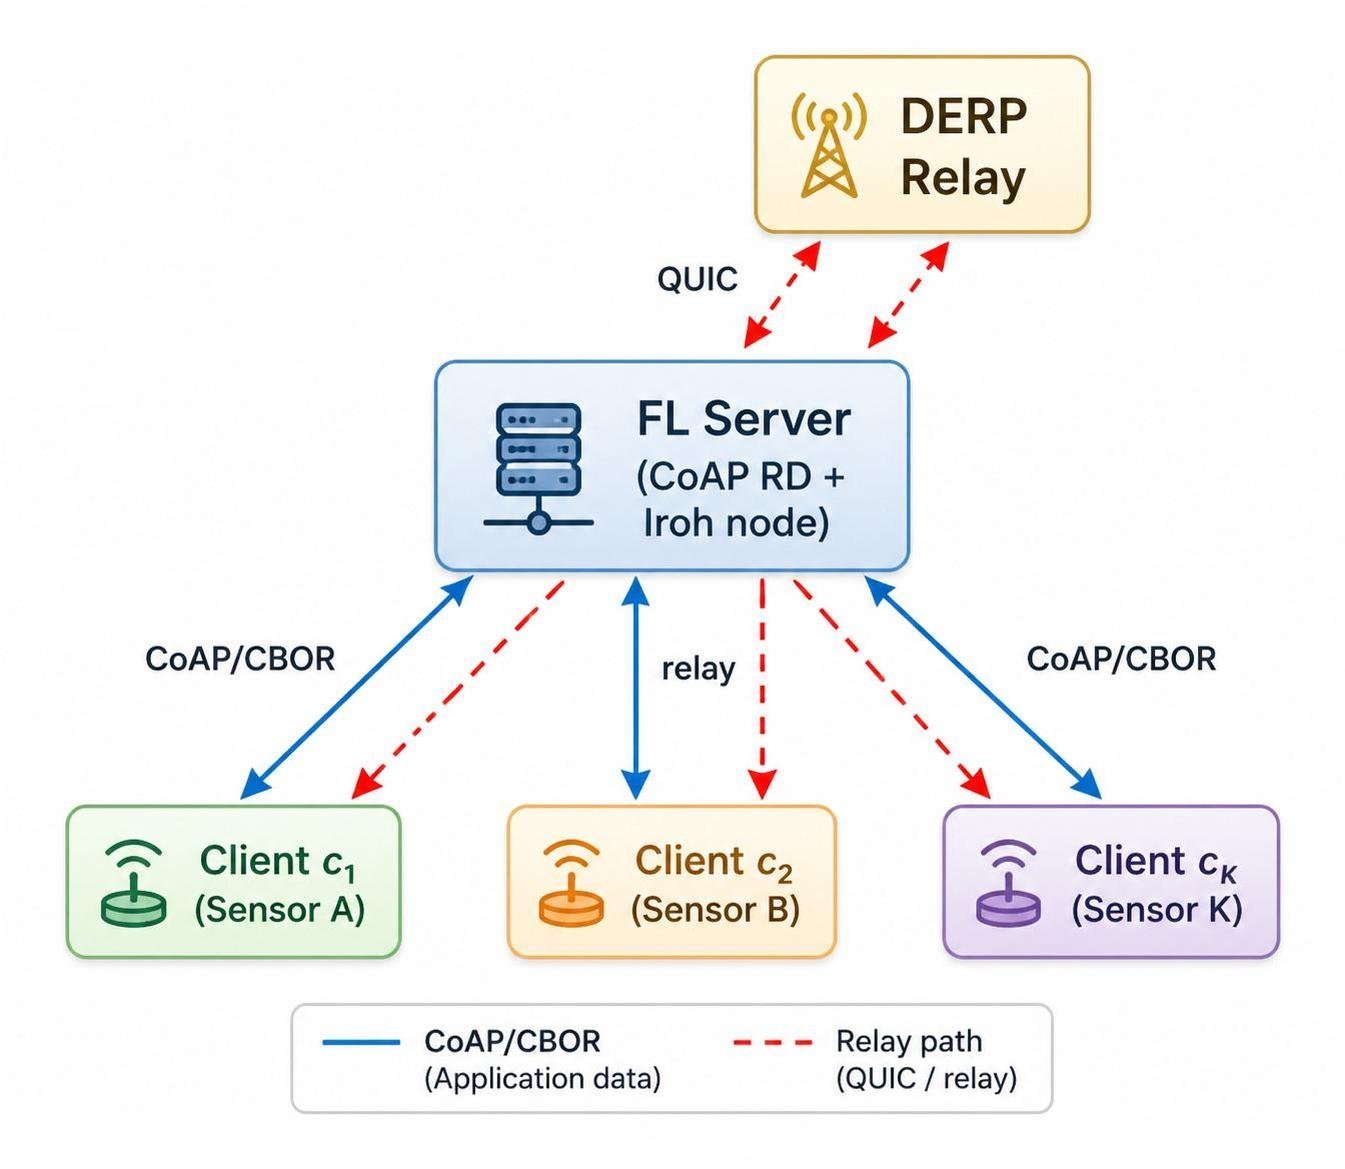
\includegraphics[width=\columnwidth]{FL-Iroh-arch.jpg}
\caption{FL-Iroh architecture. The FL server (CoAP resource directory + Iroh node) coordinates $K$ sensor clients: solid blue arrows are the \DIFdelbeginFL \DIFdelFL{CoAP/CBOR }\DIFdelendFL control plane (registration, discovery, round signaling and application metadata), while dashed red arrows are the Iroh/QUIC relay path through the DERP relay, used transparently for tensor data whenever a direct hole-punched path cannot be \DIFdelbeginFL \DIFdelFL{formed}\DIFdelendFL \DIFaddbeginFL \DIFaddFL{validated}\DIFaddendFL .}
\label{fig:architecture}
\end{figure}

\begin{figure}[t]
\centering
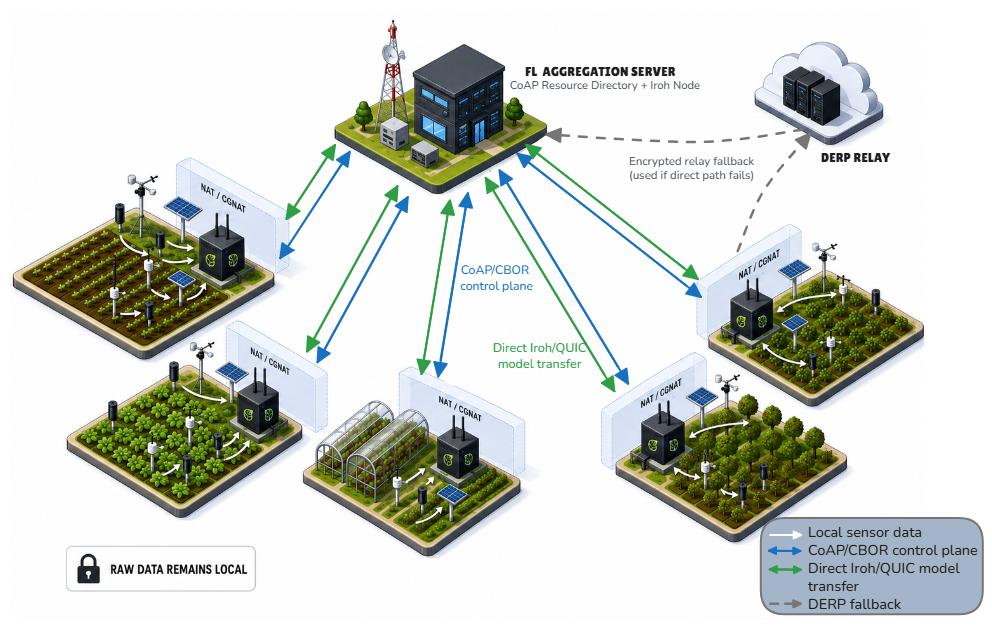
\includegraphics[width=\columnwidth]{physical-deploy.png}
\caption{Target deployment of FL-Iroh in agricultural IoT. Field sensors collect agronomic and meteorological measurements that remain within each farm and are processed by a local FL client behind NAT or CGNAT. \DIFdelbeginFL \DIFdelFL{The clients use CoAP/CBOR for registration}\DIFdelendFL \DIFaddbeginFL \DIFaddFL{Clients register with the aggregator}\DIFaddendFL , \DIFdelbeginFL \DIFdelFL{discovery}\DIFdelendFL \DIFaddbeginFL \DIFaddFL{which admits only allow-listed public keys}\DIFaddendFL , and \DIFdelbeginFL \DIFdelFL{round coordination, while }\DIFdelendFL \DIFaddbeginFL \DIFaddFL{exchange }\DIFaddendFL global models and local updates \DIFdelbeginFL \DIFdelFL{are exchanged directly with the aggregation server }\DIFdelendFL over end-to-end-encrypted Iroh/QUIC connections. If a direct hole-punched path cannot be \DIFdelbeginFL \DIFdelFL{established}\DIFdelendFL \DIFaddbeginFL \DIFaddFL{validated}\DIFaddendFL , the encrypted traffic is transparently forwarded through the DERP relay.}
\label{fig:agro}
\end{figure}

\subsection{\DIFdelbegin \DIFdel{Iroh Transport}\DIFdelend \DIFaddbegin \DIFadd{Node Identity and Admission Control}\DIFaddend }
\DIFaddbegin \label{sec:admission}

\DIFadd{Every node owns a persistent 32-byte Ed25519 secret key; its public key is the node ID used to address it. The QUIC/TLS~1.3 handshake proves possession of the secret key, so a peer cannot claim a node ID it does not own. The aggregator keeps an allow-list of authorized client node IDs (one line per member, distributed out of band when a farm joins the federation). Admission is enforced at three points: (i)~on every incoming Iroh connection, }\emph{\DIFadd{before}} \DIFadd{any stream is read, the authenticated remote node ID is checked and unknown peers are closed with an application error code; (ii)~registration (CoAP }\texttt{\DIFadd{/fl/register}}\DIFadd{, }\texttt{\DIFadd{/rd}}\DIFadd{, or }\texttt{\DIFadd{fl-ctrl/1}}\DIFadd{) is refused for node IDs outside the allow-list, and over }\texttt{\DIFadd{fl-ctrl/1}} \DIFadd{the registered endpoint must belong to the authenticated sender; (iii)~each round, the aggregator accepts at most one update per }\emph{\DIFadd{selected}} \DIFadd{node ID, discarding updates from unselected peers and duplicates. Registering an allow-listed node ID one does not own over CoAP gains nothing: models are addressed to that node ID and updates are only accepted from the peer holding its key.
}

\subsection{\DIFadd{Iroh Transport and Path Selection}}
\label{sec:transport}
\DIFaddend 

Iroh~\cite{iroh2024} creates a QUIC endpoint \DIFdelbegin \DIFdel{that embeds a }\DIFdelend \DIFaddbegin \DIFadd{whose }\DIFaddend \emph{node address} \DIFdelbegin \DIFdel{consisting of a 32-byte public key (node ID)}\DIFdelend \DIFaddbegin \DIFadd{consists of the node ID}\DIFaddend , a list of \DIFaddbegin \DIFadd{candidate }\DIFaddend direct UDP addresses \DIFaddbegin \DIFadd{(local interfaces plus the public mapping discovered via STUN-like probing)}\DIFaddend , and a DERP relay URL. When a \DIFdelbegin \DIFdel{client initiates a connection to another node , Iroh:
}%DIFDELCMD < \begin{enumerate}
%DIFDELCMD <     \item %%%
\DIFdel{Registers both parties with the DERP }\DIFdelend \DIFaddbegin \DIFadd{node dials another, Iroh (i)~uses the }\DIFaddend relay for signaling \DIFdelbegin \DIFdel{.
    }%DIFDELCMD < \item %%%
\DIFdel{Simultaneously attempts UDP hole-punching to each direct address.
    }%DIFDELCMD < \item %%%
\DIFdel{If hole-punching succeeds within a configurable timeout, }\DIFdelend \DIFaddbegin \DIFadd{and, immediately, for data; (ii)~probes the candidate direct addresses (hole punching); and (iii)~migrates }\DIFaddend the QUIC session \DIFdelbegin \DIFdel{migrates to the direct path }\DIFdelend \DIFaddbegin \DIFadd{to a direct path once a probe round trip validates it. Iroh reports the resulting path as }\emph{\DIFadd{direct}} \DIFadd{(a validated UDP path), }\emph{\DIFadd{mixed}} \DIFadd{(the relay carries traffic while a direct candidate is still being validated) or }\emph{\DIFadd{relay}}\DIFadd{. FL-Iroh records this state for every transfer, together with the active address, and we count only }\emph{\DIFadd{direct}} \DIFadd{as a hole-punched path; }\emph{\DIFadd{mixed}} \DIFadd{transfers are relay-carried}\DIFaddend .
\DIFdelbegin %DIFDELCMD < \item %%%
\DIFdel{If no direct path can be negotiated (e.g., certain restrictive symmetric-NAT mappings) , all QUIC packets are forwarded by the DERP relay transparently.
}%DIFDELCMD < \end{enumerate}
%DIFDELCMD < %%%
\DIFdelend \DIFaddbegin 

\DIFadd{Two mechanisms harden the transport for unattended operation. }\emph{\DIFadd{Transfer-level retry}}\DIFadd{: if a stream is interrupted before the receiver acknowledges it (measured on a 4G CGNAT path in \S\ref{sec:e8}), the sender reopens the connection---letting Iroh re-select a path---and resends, up to a configurable number of attempts; rejections by the peer's allow-list are not retried. }\emph{\DIFadd{Endpoint watchdog}}\DIFadd{: after a configurable number of consecutive failed transfers the Iroh endpoint is restarted with the same secret key, so the node ID and pending receivers are preserved. We added the watchdog after observing in hardware tests that, after successive network switches, the endpoint of the Iroh version we use could stop establishing connections until restarted (\S\ref{sec:e8}).
}\DIFaddend 

FL-Iroh uses ALPN-based multiplexing: \DIFdelbegin \DIFdel{multiple protocol roles (}\DIFdelend model push, update upload \DIFdelbegin \DIFdel{) }\DIFdelend \DIFaddbegin \DIFadd{and control messages }\DIFaddend share a single Iroh \DIFdelbegin \DIFdel{node }\DIFdelend \DIFaddbegin \DIFadd{endpoint }\DIFaddend without port allocation\DIFaddbegin \DIFadd{, and each ALPN has its own receive queue so that concurrent consumers never block each other}\DIFaddend .

\subsection{Wire Format}
\DIFaddbegin \label{sec:wire}
\DIFaddend 

Each QUIC unidirectional stream carries one \DIFdelbegin \DIFdel{tensor bundle:
}\begin{displaymath}
\DIFdel{\underbrace{[4\,\text{B}]}_{\text{len}} \;\; \underbrace{[\text{payload}]}_{\text{torch.save blob}} \;\; \underbrace{[32\,\text{B}]}_{\text{SHA-256}}
%DIFDELCMD < \label{eq:wire}%%%
}\end{displaymath}%DIFAUXCMD
\DIFdelend \DIFaddbegin \DIFadd{payload:
}\begin{equation}
\DIFadd{\underbrace{[4\,\text{B}]}_{\text{len}} \;\; \underbrace{[\text{payload}]}_{\text{serialized parameters}} \;\; \underbrace{[32\,\text{B}]}_{\text{SHA-256}}
\label{eq:wire}
}\end{equation}\DIFaddend 
The SHA-256 suffix in Eq.~\eqref{eq:wire} provides integrity verification at the application layer, independent of QUIC's own \DIFdelbegin \DIFdel{encryption. The payload is serialized }\DIFdelend \DIFaddbegin \DIFadd{authentication. The sender waits until the receiver has read the stream to completion before releasing the connection. The framing itself is language-neutral; the prototype serializes PyTorch }\texttt{\DIFadd{state\_dict}} \DIFadd{objects }\DIFaddend with \texttt{torch.save}, \DIFdelbegin \DIFdel{producing a self-describing binary format that handles mixed tensor types and dtypes}\DIFdelend \DIFaddbegin \DIFadd{and control messages as JSON (\S\ref{sec:agnostic})}\DIFaddend .

\subsection{CoAP Control Plane \DIFaddbegin \DIFadd{and Resource Directory}\DIFaddend }
\DIFaddbegin \label{sec:coap}
\DIFaddend 

\DIFdelbegin \DIFdel{The FL server }\DIFdelend \DIFaddbegin \DIFadd{Every node }\DIFaddend exposes CoAP resources following the CoRE \DIFdelbegin \DIFdel{resource directory}\DIFdelend \DIFaddbegin \DIFadd{link format}\DIFaddend ~\cite{rfc6690}: \DIFdelbegin %DIFDELCMD < \begin{itemize}
%DIFDELCMD <     \item %%%
\texttt{\DIFdel{/fl/register}}%DIFAUXCMD
\DIFdel{: Clients POST their Iroh endpoint JSON on startup. }%DIFDELCMD < \item %%%
\DIFdelend \DIFaddbegin \texttt{\DIFadd{/fl/capabilities}} \DIFadd{(hardware, energy state and capability tags such as sensor types, crop or region), }\texttt{\DIFadd{/iroh/endpoint}}\DIFadd{, }\DIFaddend \texttt{/fl/round}\DIFdelbegin \DIFdel{: Server PUT triggers a new training round, carrying lightweight round metadata (}\DIFdelend \DIFaddbegin \DIFadd{, }\texttt{\DIFadd{/fl/policy}}\DIFadd{, }\texttt{\DIFadd{/fl/metrics}}\DIFadd{, and }\texttt{\DIFadd{/fl/register}} \DIFadd{on the aggregator. Responses are JSON or CBOR~\mbox{%DIFAUXCMD
\cite{rfc8949}}\hskip0pt%DIFAUXCMD
, negotiated with the CoAP Accept option.
}

\DIFadd{Discovery can be performed in two ways. In }\emph{\DIFadd{probe}} \DIFadd{mode the aggregator queries }\DIFaddend \texttt{\DIFdelbegin \DIFdel{round\_id}%DIFDELCMD < \MBLOCKRIGHTBRACE%%%
\DIFdel{, }\texttt{\DIFdel{model\_hash}}%DIFAUXCMD
\DIFdel{, server node ID); clients fetch the global model tensors over Iroh}\DIFdelend /\DIFdelbegin \DIFdel{QUIC (ALPN }%DIFDELCMD < \texttt{%%%
\DIFdel{fl-model}\DIFdelend \DIFaddbegin \DIFadd{fl}\DIFaddend /\DIFdelbegin \DIFdel{1}%DIFDELCMD < \MBLOCKRIGHTBRACE%%%
\DIFdel{) .
    }%DIFDELCMD < \item %%%
\DIFdelend \DIFaddbegin \DIFadd{capabilities}} \DIFadd{of every known node and filters client-side, costing one request per node. In }\emph{\DIFadd{resource-directory}} \DIFadd{mode, following RFC~9176~\mbox{%DIFAUXCMD
\cite{rfc9176}}\hskip0pt%DIFAUXCMD
, each node registers once (POST }\DIFaddend \texttt{/\DIFdelbegin \DIFdel{fl/discover}\DIFdelend \DIFaddbegin \DIFadd{rd}\DIFaddend } \DIFdelbegin \DIFdel{: Server queries registered clients with optional semantic filtering by capability tags(e. }\DIFdelend \DIFaddbegin \DIFadd{with its tags, role, energy state, lifetime and Iroh endpoint) and the aggregator answers a single lookup, e.}\DIFaddend g.\DIFdelbegin \DIFdel{, }\texttt{\DIFdel{sensor\_type=soil}}%DIFAUXCMD
\DIFdel{).
}%DIFDELCMD < \end{itemize}
%DIFDELCMD < %%%
\DIFdelend \DIFaddbegin \DIFadd{\ GET }\texttt{\DIFadd{/rd-lookup/ep}} \DIFadd{with query }\texttt{\DIFadd{tag=agri,r3,soil\_moisture}} \DIFadd{and }\texttt{\DIFadd{min\_energy=20}}\DIFadd{, with server-side filtering on any combination of capability tags, role and energy level, optionally paged. Registrations expire after their lifetime unless refreshed. E5 compares both modes up to 5}{\DIFadd{,}}\DIFadd{000 endpoints.
}\DIFaddend 

\DIFdelbegin \DIFdel{CBOR~\mbox{%DIFAUXCMD
\cite{rfc8949} }\hskip0pt%DIFAUXCMD
encoding reduces message overhead versus JSON by 30--50\% for numerical payloads, staying within 6LoWPAN block sizes for control messages}\DIFdelend \DIFaddbegin \subsection{\DIFadd{Round Protocol}}
\label{sec:round}

\DIFadd{Fig.~\ref{fig:sequence} shows the message sequence of one round and Table~\ref{alg:round} the aggregator's logic (Algorithm~1). A client that misses a round (e.g., while disconnected) simply receives the next global model when it is selected again; late registrations are included from the next round on}\DIFaddend .

\DIFaddbegin \begin{figure}[t]
\centering
\resizebox{\columnwidth}{!}{%
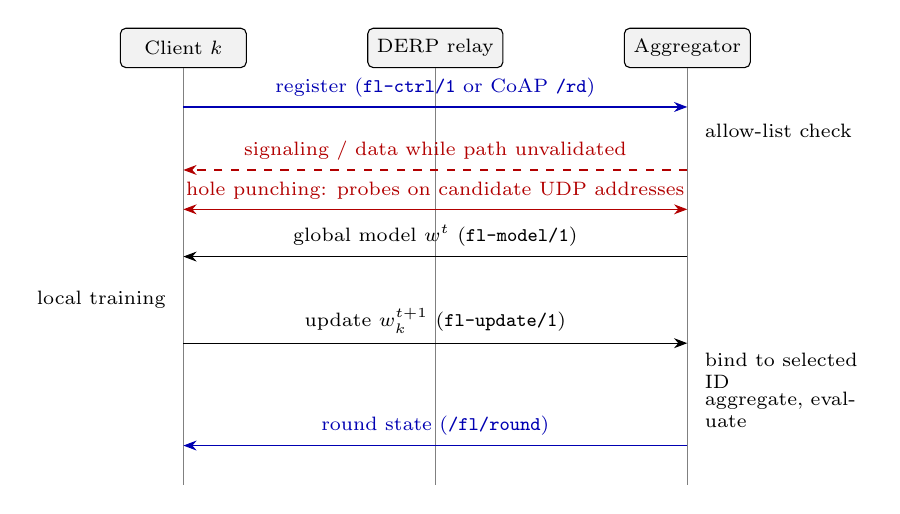
\begin{tikzpicture}[font=\scriptsize, >=Stealth,
  actor/.style={draw, rounded corners=2pt, fill=gray!10, minimum width=1.6cm, minimum height=0.5cm, align=center}]
\node[actor] (c) at (0,0) {Client $k$};
\node[actor] (r) at (3.2,0) {DERP relay};
\node[actor] (s) at (6.4,0) {Aggregator};
\foreach \n in {c,r,s} { \draw[gray] (\n.south) -- ++(0,-5.3); }
\draw[->, blue!70!black] (0,-0.75) -- node[above, pos=0.5] {register (\texttt{fl-ctrl/1} or CoAP \texttt{/rd})} (6.4,-0.75);
\node[anchor=west, align=left, text width=2.0cm] at (6.5,-1.05) {allow-list check};
\draw[->, red!70!black, dashed] (6.4,-1.55) -- node[above] {signaling / data while path unvalidated} (0,-1.55);
\draw[<->, red!70!black] (0,-2.05) -- node[above] {hole punching: probes on candidate UDP addresses} (6.4,-2.05);
\draw[->] (6.4,-2.65) -- node[above] {global model $w^{t}$ (\texttt{fl-model/1})} (0,-2.65);
\node[anchor=east, align=right] at (-0.1,-3.2) {local training};
\draw[->] (0,-3.75) -- node[above] {update $w_k^{t+1}$ (\texttt{fl-update/1})} (6.4,-3.75);
\node[anchor=west, align=left, text width=2.0cm] at (6.5,-4.1) {bind to selected ID};
\node[anchor=west, align=left, text width=2.0cm] at (6.5,-4.6) {aggregate, evaluate};
\draw[->, blue!70!black] (6.4,-5.05) -- node[above] {round state (\texttt{/fl/round})} (0,-5.05);
\end{tikzpicture}}
\caption{\DIFaddFL{Message sequence of one FL-Iroh round. Model and update streams use a validated direct path when one exists and the end-to-end-encrypted relay otherwise; the application code is identical in both cases.}}
\label{fig:sequence}
\end{figure}

\begin{table}[t]
\centering
\caption{\DIFaddFL{Algorithm~1: aggregator round $t$ (FL-Iroh server)}}
\label{alg:round}
\scriptsize
\begin{tabular}{@{}r p{7.3cm}@{}}
\toprule
1 & $S_t \leftarrow$ select clients among the admitted, registered node IDs (fraction $C$, at least $m$); \\
2 & \textbf{for} $k \in S_t$ \textbf{in parallel}: send $w^{t}$ to node ID $k$ over \texttt{fl-model/1} (retry; drop $k$ on failure); \\
3 & \textbf{if} fewer than $m$ sends succeeded \textbf{then} mark round failed and \textbf{return}; \\
4 & $U \leftarrow \emptyset$; \textbf{until} every sent $k$ answered or timeout $T$: receive $(u, \mathit{id})$ on \texttt{fl-update/1}; \\
5 & \quad \textbf{if} $\mathit{id} \in S_t$ and $\mathit{id}$ not yet in $U$ \textbf{then} $U \leftarrow U \cup \{(\mathit{id}, u)\}$ \textbf{else} discard; \\
6 & $w^{t+1} \leftarrow \texttt{aggregator\_fn}(U)$ \quad (FedAvg, FedGAM, \dots); \\
7 & evaluate $w^{t+1}$; publish round state and model descriptor on CoAP; log per-transfer path and bytes. \\
\bottomrule
\end{tabular}
\end{table}

\DIFaddend \subsection{Application Models}

\textbf{AgriMLP} (Crop Recommendation). \DIFdelbegin \DIFdel{For the crop recommendation task, we use AgriMLP: a }\DIFdelend \DIFaddbegin \DIFadd{A }\DIFaddend four-layer \DIFdelbegin \DIFdel{fully connected network (multilayer perceptron, MLP ) with architecture }\DIFdelend \DIFaddbegin \DIFadd{MLP }\DIFaddend $7 \to 64 \to 64 \to 32 \to 22$ \DIFdelbegin \DIFdel{(input features $\to$ output classes). The first two hidden layers use }\DIFdelend \DIFaddbegin \DIFadd{with }\DIFaddend Batch Normalization and Dropout (rate~0.2) \DIFdelbegin \DIFdel{for regularization. Total trainable parameters: }\DIFdelend \DIFaddbegin \DIFadd{on the first two hidden layers; }\DIFaddend 7{,}734 \DIFaddbegin \DIFadd{trainable parameters }\DIFaddend ($\approx$\DIFdelbegin \DIFdel{31~KB at float32; $\approx$}\DIFdelend 32~KB \DIFdelbegin \DIFdel{as a serializedstate dict including normalization statistics), making it trivially deployable for on-device inference on Cortex-A class hardware (Raspberry Pi~4B, Jetson Nano). Input features }\DIFdelend \DIFaddbegin \DIFadd{serialized). Inputs }\DIFaddend are z-score normalized \DIFdelbegin \DIFdel{: }\DIFdelend soil macro-nutrients (N, P, K), temperature, humidity, pH, and rainfall.

\textbf{AirMLP} (7-Day-Ahead ICA Forecasting, Outdoor). \DIFdelbegin \DIFdel{For E6 we use AirMLP, a compact }\DIFdelend \DIFaddbegin \DIFadd{A }\DIFaddend four-layer network $6 \to 32 \to 32 \to 16 \to 3$ (1{,}987 parameters, $\approx$\DIFdelbegin \DIFdel{8~KB at float32}\DIFdelend \DIFaddbegin \DIFadd{14~KB serialized}\DIFaddend ) with the same regularization scheme\DIFdelbegin \DIFdel{as AgriMLP}\DIFdelend . Inputs are daily outdoor measurements at time~$t$ (NO$_2$, O$_3$, particulate matter, CO) fused with \DIFaddbegin \DIFadd{AEMET }\DIFaddend meteorological predictors (wind speed\DIFdelbegin \DIFdel{and precipitation)from AEMET, the Spanish State Meteorological Agency, all z-score normalized. The task is to predict }\DIFdelend \DIFaddbegin \DIFadd{, precipitation); the target is }\DIFaddend the ICA class \DIFdelbegin \DIFdel{(\'Indice de Calidad del Aire, the Spanish air-quality index) 7~days ahead (}\DIFdelend \DIFaddbegin \DIFadd{at }\DIFaddend $t{+}7$ \DIFdelbegin \DIFdel{); the full task definition, labeling scheme, and rationale are given in \S\ref{sec:e6}. This model applies to open-air monitoring stations only, not indoor or greenhouse installations}\DIFdelend \DIFaddbegin \DIFadd{(\S\ref{sec:e6})}\DIFaddend .

\textbf{ProphetWrapper} (Federated GAM \DIFdelbegin \DIFdel{). FL-Iroh's transport layer is statistically model-agnostic: it serializes any }\texttt{\DIFdel{torch.state\_dict()}} %DIFAUXCMD
\DIFdel{over Iroh/QUIC without interpreting parameter semantics. We exploit this to federate }\DIFdelend \DIFaddbegin \DIFadd{case study). We wrap }\DIFaddend Facebook Prophet~\cite{taylor2018prophet} \DIFdelbegin \DIFdel{, a GAM, by wrapping it }\DIFdelend in an \texttt{nn.Module} adapter \DIFdelbegin \DIFdel{. The wrapper exposes a compatible }\texttt{\DIFdel{state\_dict()}}%DIFAUXCMD
\DIFdel{/}\texttt{\DIFdel{load\_state\_dict()}} %DIFAUXCMD
\DIFdel{interface that extracts and injects }\DIFdelend \DIFaddbegin \DIFadd{that exposes }\DIFaddend the Fourier seasonality coefficients (annual: $N{=}10$ sin/cos pairs; weekly: $N{=}3$) and the wind-speed regressor weight as \DIFdelbegin \DIFdel{floating-point tensors. Trend parameters }\DIFdelend \DIFaddbegin \DIFadd{tensors. Under }\textbf{\DIFadd{FedGAM}} \DIFadd{only these shared seasonal terms are averaged (weighted by sample count), while each zone keeps its locally fitted trend }\DIFaddend ($k$, $m$, $\delta$)\DIFdelbegin \DIFdel{encode zone-specific industrial and demographic emission patterns (e.g., Ponferrada coal plant vs.\ rural Soria) and are therefore }\emph{\DIFdel{not}} %DIFAUXCMD
\DIFdel{federated; they remain local to each zone client. This design, which we term }\textbf{\DIFdel{FedGAM}}%DIFAUXCMD
\DIFdel{, federates only the shared periodic structure of pollutant cycles while preserving local trend identity---a separation consistent with the seasonal structure documented for this dataset in prior work~\mbox{%DIFAUXCMD
\cite{lopezblanco2024airquality}}\hskip0pt%DIFAUXCMD
.
}%DIFDELCMD < 

%DIFDELCMD < %%%
\DIFdel{The current FL client requires Python~3.11 and PyTorch; porting to Cortex-M MCU-class platforms would require a C or Rust reimplementation of the client runtime.
}\DIFdelend \DIFaddbegin \DIFadd{; under FedAvg all parameters are averaged. Formally, with $\theta_k = (\theta_k^{s}, \theta_k^{\tau})$ the seasonal and trend parameters of zone $k$ and $n_k$ its sample count,
}\begin{equation}
\DIFadd{\theta^{s} \leftarrow \sum_k \frac{n_k}{\sum_j n_j}\,\theta_k^{s}, \qquad \theta_k^{\tau} \text{ kept local}.
\label{eq:fedgam}
}\end{equation}
\DIFaddend 

% =========================================================================
\section{Experimental Evaluation}
\label{sec:evaluation}

We report \DIFdelbegin \DIFdel{six experiments (E1--E6}\DIFdelend \DIFaddbegin \DIFadd{eleven experiments (Table~\ref{tab:explist}}\DIFaddend ) followed by an operational comparison with Flower-over-Tailscale (\S\DIFdelbegin \DIFdel{\ref{sec:e7}}\DIFdelend \DIFaddbegin \DIFadd{\ref{sec:flower}}\DIFaddend ). Throughout, we distinguish \DIFdelbegin \DIFdel{two connectivity metrics: }\emph{\DIFdel{session-level establishment}} %DIFAUXCMD
\DIFdel{(whether a usable connection is eventually formed, including retries) and the }\DIFdelend \DIFaddbegin \DIFadd{three connectivity outcomes for every transfer or connection attempt: }\DIFaddend \emph{\DIFdelbegin \DIFdel{per-transfer direct-path rate}\DIFdelend \DIFaddbegin \DIFadd{direct}\DIFaddend } (\DIFdelbegin \DIFdel{the fraction of individual transfers }\DIFdelend carried over a \DIFaddbegin \DIFadd{validated }\DIFaddend hole-punched \DIFdelbegin \DIFdel{path rather than the relay)}\DIFdelend \DIFaddbegin \DIFadd{UDP path), }\emph{\DIFadd{relay-carried}} \DIFadd{(Iroh state }\emph{\DIFadd{relay}} \DIFadd{or }\emph{\DIFadd{mixed}}\DIFadd{, i.e., the DERP relay carries the traffic while no direct path is validated), and }\emph{\DIFadd{failed}}\DIFaddend .

\DIFaddbegin \begin{table}[t]
\centering
\caption{\DIFaddFL{Experiments, research questions and reviewer-requested additions in this revision}}
\label{tab:explist}
\scriptsize
\setlength{\tabcolsep}{2.5pt}
\begin{tabular}{@{}l p{4.1cm} l l@{}}
\toprule
\textbf{Exp.} & \textbf{Question} & \textbf{Platform} & \textbf{Transport} \\
\midrule
E1 & Transport throughput (relay path) & PC, RPi & real Iroh \\
E2 & Convergence under non-IID data & HPC & in-process \\
E3 & Connection establishment across classified NATs & PC, RPi & real Iroh \\
E4 & Robustness to client dropout (simulated) & HPC & in-process \\
E5 & CoAP discovery scaling to 5{,}000 endpoints & PC & CoAP \\
E6 & Air-quality forecasting, imbalance-aware metrics & HPC, PC & real Iroh \\
E7 & Operational comparison with Flower + Tailscale (\S\ref{sec:flower}) & HPC & in-process \\
E8 & Forced relay, outages, network switches & RPi, PC & real Iroh \\
E9 & Loss / latency / bandwidth sweep & PC (netem) & real Iroh \\
E10 & Public-key admission control & PC, RPi & real Iroh \\
E11 & Full federation over WAN; RPi resources & RPi, PC & real Iroh \\
\bottomrule
\end{tabular}
\end{table}

\DIFaddend \subsection{Experimental Setup}
\DIFaddbegin \label{sec:setup}
\DIFaddend 

\DIFdelbegin \DIFdel{All experiments }\DIFdelend \DIFaddbegin \textbf{\DIFadd{Hardware.}} \DIFadd{The edge client is a Raspberry Pi~3 Model~B (quad-core Cortex-A53 at 1.2~GHz, 1~GB RAM; Raspberry Pi OS based on Debian~13, Python~3.13, PyTorch~2.12 CPU build). The aggregator is a laptop PC running the server inside WSL2 (Ubuntu) on Windows~11. Learning-dynamics experiments (E2, E4 and the multi-seed part of E6) }\DIFaddend run on a single-node HPC cluster (Intel Xeon, 16 cores, no GPU)\DIFdelbegin \DIFdel{for E2, E4, E5, E6, and on real hardware (PC with Windows Subsystem for Linux 2, WSL2, + Raspberry Pi~4B}\DIFdelend \DIFaddbegin \DIFadd{. All experiments use the Iroh~0.35 Python bindings and the public n0 DERP relays.
}

\textbf{\DIFadd{Networks.}} \DIFadd{Table~\ref{tab:networks} lists the networks used in the hardware experiments. For the networks added in this revision we measured NAT mapping and filtering behavior with RFC~4787/RFC~5780 STUN probes from the device itself (}\texttt{\DIFadd{scripts/nat\_classify.py}} \DIFadd{in the artifact): mapping is classified by querying five STUN servers on different IPs from one local UDP port, and filtering by RFC~5780 CHANGE-REQUEST tests. The earlier cross-ISP campaign (PC~$\leftrightarrow$~Raspberry Pi}\DIFaddend , 300~km \DIFdelbegin \DIFdel{WAN separation) for E1 distributed and E3.
}\DIFdelend \DIFaddbegin \DIFadd{apart) used router/ISP configurations that were labeled but not probed; we keep those labels as descriptions of the configured topology.
}

\begin{table}[t]
\centering
\caption{\DIFaddFL{Networks used in the hardware experiments (RFC~4787 behavior measured with STUN probes; EIM = endpoint-independent mapping; ADF = address-dependent filtering)}}
\label{tab:networks}
\scriptsize
\setlength{\tabcolsep}{2.5pt}
\begin{tabular}{@{}l p{3.0cm} l l l@{}}
\toprule
\textbf{Id} & \textbf{Network} & \textbf{Mapping} & \textbf{Filtering} & \textbf{Port pres.} \\
\midrule
N1 & Office Wi-Fi (enterprise NAT) & EIM & ADF & yes \\
N2 & Mobile 4G (Lowi/Vodafone) via phone hotspot: hotspot NAT + carrier NAT & EIM & ADF & no \\
N3 & Home fixed broadband (host OS) & EIM & ADF & yes \\
N3$'$ & N3 seen from WSL2 (additional host NAT) & EIM & ADF & no \\
\midrule
C1--C5 & Earlier cross-ISP campaign: base, ``full-cone'', ``symmetric'', CGNAT (mobile carrier), port-443 firewall & \multicolumn{3}{l}{configured, not probed} \\
\bottomrule
\end{tabular}
\end{table}

\textbf{\DIFadd{Software and data.}} \DIFaddend FL experiments use $K{=}10$ clients \DIFdelbegin \DIFdel{with }\DIFdelend \DIFaddbegin \DIFadd{unless stated, }\DIFaddend FedAvg (or FedGAM for \DIFdelbegin \DIFdel{E6-Prophet}\DIFdelend \DIFaddbegin \DIFadd{the Prophet case study}\DIFaddend ), $E{=}1$ local epoch\DIFdelbegin \DIFdel{per round, SGD optimizer }\DIFdelend \DIFaddbegin \DIFadd{, SGD }\DIFaddend (lr$=$0.01\DIFaddbegin \DIFadd{, momentum 0.9, weight decay $10^{-4}$}\DIFaddend ), and $R{=}100$ \DIFdelbegin \DIFdel{global }\DIFdelend rounds for E2 and E4, $R{=}50$ for E6\DIFaddbegin \DIFadd{, $R{=}20$ for E9 and $R{=}30$ for E11}\DIFaddend . E2 uses SimpleCNN \DIFdelbegin \DIFdel{, a three-block convolutional network (}\DIFdelend \DIFaddbegin \DIFadd{(three }\DIFaddend Conv--BN--ReLU blocks of 32/64/128 channels\DIFdelbegin \DIFdel{with max-pooling}\DIFdelend , global average pooling \DIFdelbegin \DIFdel{, }\DIFdelend and a linear head; 94{,}762 \DIFdelbegin \DIFdel{trainable parameters, $\approx$0.38~MB serialized state dict}\DIFdelend \DIFaddbegin \DIFadd{parameters}\DIFaddend ) on CIFAR-10~\cite{cifar2009}. The Crop Recommendation dataset~\cite{cropdataset} contains 2\DIFdelbegin \DIFdel{,}\DIFdelend \DIFaddbegin {\DIFadd{,}}\DIFaddend 200 records across 22 \DIFdelbegin \DIFdel{crop classes(100 records/class), partitioned using Dirichlet allocation with concentration }\DIFdelend \DIFaddbegin \DIFadd{classes, partitioned IID or with Dirichlet }\DIFaddend $\alpha \in \{0.1, 0.5, 1.0\}$\DIFdelbegin \DIFdel{and IID as a baseline}\DIFdelend . The E6 \DIFdelbegin \DIFdel{air quality }\DIFdelend \DIFaddbegin \DIFadd{air-quality }\DIFaddend dataset covers 10 Castilla y Le\'on monitoring \DIFdelbegin \DIFdel{zones---the nine provincial capitals plus Ponferrada---over }\DIFdelend \DIFaddbegin \DIFadd{zones over }\DIFaddend 2011--2019 (train: 2011--2018, test: 2019) with a geographic partition (one client per zone) and an IID \DIFdelbegin \DIFdel{shuffled }\DIFdelend baseline. Multi-seed runs use a fixed \DIFdelbegin \DIFdel{replication-seed }\DIFdelend \DIFaddbegin \DIFadd{seed }\DIFaddend registry ($n{=}5$\DIFdelbegin \DIFdel{seeds}\DIFdelend ); 95\% confidence intervals use the Student-$t$ distribution.
\DIFdelbegin \DIFdel{Code and data }\DIFdelend \DIFaddbegin 

\textbf{\DIFadd{Transport in each experiment.}} \DIFadd{E2 and E4 study learning dynamics (non-IID data, partial participation) and were run with an in-process loopback transport that delivers the same serialized payloads without the network stack; we report them as statistical experiments and evaluate all transport behavior on real Iroh connections in E1, E3, E6 and E8--E11. Code, per-run results and analysis scripts }\DIFaddend are available at the anonymized project repository (URL withheld for double-blind review).

\subsection{E1: Transport Throughput}
\label{sec:e1}

We benchmark three transport configurations across four payload sizes (100~KB, 1~MB, 10~MB, 100~MB):

\begin{itemize}
    \item \textbf{HTTP/2 (loopback)}: aiohttp server+client on localhost, serving as a ceiling baseline.
    \item \textbf{iroh\_relay\_loopback}: \DIFdelbegin \DIFdel{Two }\DIFdelend \DIFaddbegin \DIFadd{two }\DIFaddend in-process Iroh nodes on the same machine, using the public DERP relay \texttt{euw1-1.relay.iroh.network}.
    \item \textbf{iroh\_relay\_wan}: PC as server and \DIFdelbegin \DIFdel{Raspberry Pi~4B }\DIFdelend \DIFaddbegin \DIFadd{the Raspberry Pi }\DIFaddend (300~km \DIFdelbegin \DIFdel{geographic separation, different ISPs}\DIFdelend \DIFaddbegin \DIFadd{away, different ISP}\DIFaddend ) as client, using the same public DERP relay.
\DIFdelbegin \DIFdel{The separation ensures no shared routing infrastructure, representing a realistic worst-case WAN scenario.
}\DIFdelend \end{itemize}

Results are shown in Table~\ref{tab:e1}. HTTP/2 peaks at 573~Mbps for 1~MB payloads on loopback, dropping to 244~Mbps at 100~MB (memory bandwidth limited). The iroh relay loopback achieves 27.2~Mbps at 100~KB ($N{=}14$, preliminary)\DIFdelbegin \DIFdel{, reflecting QUIC+relay encryption overhead on a fast local path}\DIFdelend . The WAN relay saturates at 2.8~Mbps independent of payload size ($N{=}30$ per cell)\DIFdelbegin \DIFdel{. For AgriMLP model exchanges ($\approx$31~KB per direction), transport time over the WAN relay is $\approx$110~ms per push and $\approx$220~ms for a full download-plus-upload exchange, yielding $<$1~s per federated round at the network level. Note that Table~\ref{tab:e1} characterizes the }\emph{\DIFdel{relay}} %DIFAUXCMD
\DIFdel{path, which E3 shows to be the uncommon fallback case; direct hole-punched paths avoid the relay hop entirely and are bounded by the end-to-end link capacity instead.
}%DIFDELCMD < 

%DIFDELCMD < \begin{table}[t]
%DIFDELCMD < \centering
%DIFDELCMD < %%%
%DIFDELCMD < \caption{%
{%DIFAUXCMD
\DIFdelFL{E1: Transport Throughput Summary}}
%DIFAUXCMD
%DIFDELCMD < \label{tab:e1}
%DIFDELCMD < \scriptsize
%DIFDELCMD < \setlength{\tabcolsep}{3.5pt}
%DIFDELCMD < \begin{tabular}{l r r r r}
%DIFDELCMD < \toprule
%DIFDELCMD < \textbf{Transport} & \textbf{Payload} & \textbf{Mean (Mbps)} & \textbf{P95 (Mbps)} & \textbf{N} \\
%DIFDELCMD < \midrule
%DIFDELCMD < HTTP/2               & 100~KB  & 208.2  & 245.5  & 30 \\
%DIFDELCMD < HTTP/2               & 1~MB    & 573.6  & 603.3  & 30 \\
%DIFDELCMD < HTTP/2               & 10~MB   & 479.2  & 560.3  & 30 \\
%DIFDELCMD < HTTP/2               & 100~MB  & 244.6  & 248.9  & 30 \\
%DIFDELCMD < \midrule
%DIFDELCMD < iroh relay loopback  & 100~KB  & 27.2   & 29.2   & 14 \\
%DIFDELCMD < \midrule
%DIFDELCMD < iroh relay WAN       & 100~KB  & 2.26   & 2.43   & 30 \\
%DIFDELCMD < iroh relay WAN       & 1~MB    & 2.75   & 2.79   & 30 \\
%DIFDELCMD < iroh relay WAN       & 10~MB   & 2.81   & 2.82   & 30 \\
%DIFDELCMD < iroh relay WAN       & 100~MB  & 2.81   & 2.83   & 30 \\
%DIFDELCMD < \bottomrule
%DIFDELCMD < \end{tabular}
%DIFDELCMD < \end{table}
%DIFDELCMD < 

%DIFDELCMD < %%%
\DIFdel{The flat throughput curve across payloads (100~KB to 100~MB all saturate at $\approx$2.8~Mbps, $N{=}30$ per cell, stdev${<}$0.05~Mbps) }\DIFdelend \DIFaddbegin \DIFadd{, which }\DIFaddend points to a relay-side \DIFdelbegin \DIFdel{ceiling---server }\DIFdelend \DIFaddbegin \DIFadd{ceiling (server }\DIFaddend capacity or per-connection rate limiting on the public \DIFdelbegin \DIFdel{relay---rather than QUIC protocol }\DIFdelend \DIFaddbegin \DIFadd{relay) rather than QUIC }\DIFaddend overhead; we did not benchmark a self-hosted \DIFdelbegin \DIFdel{DERP }\DIFdelend relay to separate the two\DIFdelbegin \DIFdel{explanations. Either way, a self-hosted relay on a dedicated server would lift this ceiling, and the public relay already suffices for AgriMLP-sized model updates ($\approx$220~ms per round-trip exchange) }\DIFdelend \DIFaddbegin \DIFadd{. In E8 the relay delivered 1~MB updates at a median 1.85~Mbps over a 4G uplink, essentially the same as the direct path on that link (1.88~Mbps), so on mobile links the access network rather than the relay was the bottleneck. For AgriMLP and AirMLP updates (14--32~KB) relay transport time is a few hundred milliseconds per round}\DIFaddend .

\DIFaddbegin \begin{table}[t]
\centering
\caption{\DIFaddFL{E1: Transport Throughput Summary}}
\label{tab:e1}
\scriptsize
\setlength{\tabcolsep}{3.5pt}
\begin{tabular}{l r r r r}
\toprule
\textbf{Transport} & \textbf{Payload} & \textbf{Mean (Mbps)} & \textbf{P95 (Mbps)} & \textbf{N} \\
\midrule
HTTP/2               & 100~KB  & 208.2  & 245.5  & 30 \\
HTTP/2               & 1~MB    & 573.6  & 603.3  & 30 \\
HTTP/2               & 10~MB   & 479.2  & 560.3  & 30 \\
HTTP/2               & 100~MB  & 244.6  & 248.9  & 30 \\
\midrule
iroh relay loopback  & 100~KB  & 27.2   & 29.2   & 14 \\
\midrule
iroh relay WAN       & 100~KB  & 2.26   & 2.43   & 30 \\
iroh relay WAN       & 1~MB    & 2.75   & 2.79   & 30 \\
iroh relay WAN       & 10~MB   & 2.81   & 2.82   & 30 \\
iroh relay WAN       & 100~MB  & 2.81   & 2.83   & 30 \\
\bottomrule
\end{tabular}
\end{table}

\DIFaddend \subsection{E2: FL Convergence Under Non-IID Data}
\label{sec:e2}

We evaluate FedAvg convergence on CIFAR-10 with SimpleCNN under IID and non-IID (Dirichlet $\alpha{=}0.1$) partitioning \DIFdelbegin \DIFdel{. All runs use }\DIFdelend \DIFaddbegin \DIFadd{(}\DIFaddend $K{=}10$\DIFdelbegin \DIFdel{clients}\DIFdelend , $E{=}1$\DIFdelbegin \DIFdel{local epoch, cross-entropy loss, SGD optimizer (lr$=$0.01)}\DIFdelend , $R{=}100$\DIFdelbegin \DIFdel{rounds. Multi-seed replication (}\DIFdelend \DIFaddbegin \DIFadd{, }\DIFaddend $n{=}5$ \DIFdelbegin \DIFdel{) provides 95\% confidence intervals via Student-t distribution. Results in }\DIFdelend \DIFaddbegin \DIFadd{seeds; }\DIFaddend Table~\ref{tab:e2}\DIFaddbegin \DIFadd{)}\DIFaddend .

\begin{table}[t]
\centering
\caption{E2: FL Convergence on CIFAR-10 (SimpleCNN, $K{=}10$, $R{=}100$, $n{=}5$ seeds)}
\label{tab:e2}
\footnotesize
\begin{tabular}{l r r}
\toprule
\textbf{Partition} & \textbf{Test Acc. (final)} & \textbf{95\% CI} \\
\midrule
IID                  & 65.86\% & [65.66\%, 66.06\%] \\
Dirichlet $\alpha{=}0.1$ & 44.18\% & [39.45\%, 48.92\%] \\
\bottomrule
\end{tabular}
\end{table}

Under IID partitioning, SimpleCNN converges to 65.86\% test accuracy with a \DIFdelbegin \DIFdel{tight }\DIFdelend 95\% CI of $\pm$0.2pp\DIFdelbegin \DIFdel{($n{=}5$ seeds), demonstrating reproducible convergence. Severe non-IID heterogeneity }\DIFdelend \DIFaddbegin \DIFadd{. Severe label skew }\DIFaddend (Dirichlet $\alpha{=}0.1$) \DIFdelbegin \DIFdel{causes substantial degradation }\DIFdelend \DIFaddbegin \DIFadd{lowers accuracy }\DIFaddend to 44.18\% \DIFdelbegin \DIFdel{, }\DIFdelend with a wider CI \DIFdelbegin \DIFdel{of }\DIFdelend \DIFaddbegin \DIFadd{(}\DIFaddend $\pm$4.7pp\DIFdelbegin \DIFdel{reflecting increased variance across different client-data assignments. The 21.7pp accuracy gap quantifies the cost of label skew in CIFAR-10 FL}\DIFdelend \DIFaddbegin \DIFadd{)}\DIFaddend , consistent with prior work~\cite{li2020federated,scaffold2020}. \DIFdelbegin \DIFdel{Despite heterogeneity, FedAvg converges without divergence, validating the robustness of the transport layer under realistic non-IID conditions.
}%DIFDELCMD < 

%DIFDELCMD < %%%
\DIFdel{A heterogeneity sweep over the Dirichlet concentration parameter (}\DIFdelend \DIFaddbegin \DIFadd{A }\DIFaddend single-seed \DIFdelbegin \DIFdel{runs) confirms the expected monotonic trend : accuracy degrades smoothly }\DIFdelend \DIFaddbegin \DIFadd{sweep confirms a monotonic trend }\DIFaddend from IID (65.86\%) through $\alpha{=}1.0$ (63.95\%) and $\alpha{=}0.5$ (62.64\%) to \DIFdelbegin \DIFdel{the severe }\DIFdelend $\alpha{=}0.1$\DIFdelbegin \DIFdel{regime, where label skew becomes the dominant error source. The transport layer imposes no additional convergence penalty at any heterogeneity level: all }\DIFdelend \DIFaddbegin \DIFadd{. All }\DIFaddend runs complete their \DIFdelbegin \DIFdel{full }\DIFdelend 100 rounds\DIFdelbegin \DIFdel{with 100\% round-level success and an identical per-round byte cost of }\DIFdelend \DIFaddbegin \DIFadd{; each round aggregates }\DIFaddend 3.87~MB of \DIFdelbegin \DIFdel{aggregated client updates ($K{=}10$ }\DIFdelend updates \DIFdelbegin \DIFdel{$\times$ $\approx$}\DIFdelend \DIFaddbegin \DIFadd{($K{=}10 \times \approx$}\DIFaddend 0.387~MB\DIFdelbegin \DIFdel{serialized SimpleCNN state dict each}\DIFdelend ).

\subsection{E3: \DIFdelbegin \DIFdel{NAT Traversal Success Rate}\DIFdelend \DIFaddbegin \DIFadd{Connection Establishment Across Classified NATs}\DIFaddend }
\label{sec:e3}

\DIFdelbegin \DIFdel{We measure connection establishment success and, where the transport API exposes it, the connection type (direct hole-punch vs.~relay) across five network scenarios using real hardware:
}%DIFDELCMD < 

%DIFDELCMD < \begin{itemize}
\begin{itemize}%DIFAUXCMD
%DIFDELCMD <     \item %%%
\item%DIFAUXCMD
\textbf{\DIFdel{net\_lan}}%DIFAUXCMD
\DIFdel{: both peers on the same local network (control baseline).
    }%DIFDELCMD < \item %%%
\item%DIFAUXCMD
\textbf{\DIFdel{net\_nat1}} %DIFAUXCMD
\DIFdel{(full-cone NAT): PC behind a standard home router (Spain) $\leftrightarrow$ Raspberry Pi~4B (remote location, 300~km).
    }%DIFDELCMD < \item %%%
\item%DIFAUXCMD
\textbf{\DIFdel{net\_nat2}} %DIFAUXCMD
\DIFdel{(symmetric NAT): a second NAT topology with a different router pairing.
    }%DIFDELCMD < \item %%%
\item%DIFAUXCMD
\textbf{\DIFdel{net\_cgnat}} %DIFAUXCMD
\DIFdel{(Carrier-Grade NAT): same hardware, with the PC behind an ISP-level CGNAT.
    }%DIFDELCMD < \item %%%
\item%DIFAUXCMD
\textbf{\DIFdel{net\_fw443}} %DIFAUXCMD
\DIFdel{(restrictive firewall): outbound traffic constrained to port~443 only, with both UDP/443 and TCP/443 permitted---so a direct QUIC pathon UDP/443 remains possible and the HTTPS relay uses TCP/443. (The repository additionally ships a stricter }\emph{\DIFdel{emulated}} %DIFAUXCMD
\DIFdel{variant of this scenario that blocks all UDP and therefore forces relay-only operation; that variant was not used in these physical runs.)
}
\end{itemize}%DIFAUXCMD
%DIFDELCMD < \end{itemize}
%DIFDELCMD < 

%DIFDELCMD < %%%
\DIFdel{Each scenario runs $N{=}30$ transfers over a single established session (1--3 distinct QUIC connections per run), so the unit of analysis in Table~\ref{tab:e3} is the }\DIFdelend \DIFaddbegin \paragraph{\DIFadd{Correction of the path classification.}} \DIFadd{The original submission counted Iroh's }\emph{\DIFadd{mixed}} \DIFadd{state as a direct path. While analysing the forced-relay experiments of this revision (\S\ref{sec:e8}), we found that with all outgoing UDP blocked---so that hole punching is impossible---Iroh reports the connection as }\DIFaddend \emph{\DIFdelbegin \DIFdel{transfer}\DIFdelend \DIFaddbegin \DIFadd{mixed}\DIFaddend }, not \DIFdelbegin \DIFdel{an independent connection-establishment attempt: across the four WAN scenarios the 120 transfers correspond to roughly 4--12 distinct QUIC connections on one PC$\leftrightarrow$Raspberry~Pi hardware pair. Transfer-level percentages therefore measure the stability of the direct path during operation; they should not be read as a population-level hole-punching success probability (see \S\ref{sec:limitations}). Results are shown in Table~\ref{tab:e3}.
}%DIFDELCMD < 

%DIFDELCMD < \begin{table*}[t]
%DIFDELCMD < \centering
%DIFDELCMD < %%%
%DIFDELCMD < \caption{%
{%DIFAUXCMD
\DIFdelFL{E3: NAT Traversal Results ($N{=}30$ transfers per scenario, one established session each; connection path classified via Iroh }\texttt{\DIFdelFL{remote\_info()}} %DIFAUXCMD
\DIFdelFL{active-path inspection)}}
%DIFAUXCMD
%DIFDELCMD < \label{tab:e3}
%DIFDELCMD < \footnotesize
%DIFDELCMD < \begin{tabular}{l r r r r l}
%DIFDELCMD < \toprule
%DIFDELCMD < \textbf{Scenario} & \textbf{$N$} & \textbf{Direct (\%)} & \textbf{Relay (\%)} & \textbf{Failed (\%)} & \textbf{Active path} \\
%DIFDELCMD < \midrule
%DIFDELCMD < net\_lan   (LAN baseline)   & 30 & 100.0 & 0.0 & 0.0 & direct (local)  \\
%DIFDELCMD < net\_nat1  (full-cone NAT)  & 30 & 96.7  & 0.0 & 3.3 & direct (public) \\
%DIFDELCMD < net\_nat2  (symmetric NAT)  & 30 & 100.0 & 0.0 & 0.0 & direct (public) \\
%DIFDELCMD < net\_cgnat (CGNAT)          & 30 & 96.7  & 0.0 & 3.3 & direct (public) \\
%DIFDELCMD < net\_fw443 (firewall :443)  & 30 & 100.0 & 0.0 & 0.0 & direct (public) \\
%DIFDELCMD < \midrule
%DIFDELCMD < \textbf{WAN aggregate}      & 120 & \textbf{98.3} & \textbf{0.0} & 1.7 & direct (public) \\
%DIFDELCMD < \bottomrule
%DIFDELCMD < \end{tabular}
%DIFDELCMD < \end{table*}
%DIFDELCMD < 

%DIFDELCMD < %%%
\DIFdel{The key result: direct QUIC hole-punching carried every completed WAN transfer in every NAT, CGNAT, and firewall scenario---with 0\% relay usage. Of 120 WAN transfers (four scenarios $\times$ 30), 118 (98.3\%) rode a }\DIFdelend \DIFaddbegin \emph{\DIFadd{relay}}\DIFadd{: it keeps a direct candidate address while the relay carries all traffic. Debug logs of every cold start record, for each candidate address, whether a probe round trip has been measured; in all }\emph{\DIFadd{mixed}} \DIFadd{cases no candidate had one, i.e., no direct path had been validated. We therefore re-classified the original campaign with the strict criterion (direct = Iroh reports }\DIFaddend \emph{direct} \DIFdelbegin \DIFdel{peer-to-peer path and none fell back to the DERP relay ; the two failures (1.7\%) were first-attempt cold-start timeouts that succeeded on retry within the same session, so session-level establishment was 100\%. In every direct connection the active wire address was the remote peer's }\emph{\DIFdel{public}} %DIFAUXCMD
\DIFdel{IP, not a private LAN address---confirming a genuine hole-punched WAN path rather than a co-located shortcut. For the CGNAT scenario we additionally verified network isolation by confirming the two peers' private subnets were mutually unreachable (100\% packet loss), with the PC on a mobile-carrier CGNAT and the Raspberry Pi 300~km away on a different fixed ISP. Direct connectivity thus held even under Carrier-Grade NAT, symmetric NAT, and a port-443-only firewall, cross-ISP.As a control, the same-LAN baseline (net\_lan, both peers co-located) instead reported the peer's }\emph{\DIFdel{private}} %DIFAUXCMD
\DIFdel{RFC1918 address with sub-50~ms latency (15--47~ms vs.~62--625~ms over WAN), confirming that the active-path classifier faithfully distinguishes a local direct path from a WAN hole-punched one rather than defaulting to a public address. }%DIFDELCMD < 

%DIFDELCMD < %%%
\DIFdel{Session bring-up in the transfer campaign was highly variable: the server-side interval from listener start to the session's first accepted connection ranged from 5.3~s (CGNAT) to 114~s (symmetric NAT) . This interval includes client process bootstrap, relay-assisted rendezvous discovery, and any first-attempt retries---not just QUIC dialing---so it upper-bounds rather than measures connection establishment proper; the dedicated cold-start campaign belowisolates the establishment interval itself (client-side, dial to established connection), whose medians are two orders of magnitude smaller. Once established, steady-state transfer latency is low (62--625~ms, typically $<$300~ms), and subsequent transfers reuse the direct path. These latencies are acceptable for FL model exchange, where local training dominates round time.
}%DIFDELCMD < 

%DIFDELCMD < %%%
\DIFdel{This result is stronger than the relay-fallback guarantee alone: Iroh's hole-punching formed direct paths even under the symmetric-NAT and CGNAT conditions that classically defeat it. The DERP relay remains a }\emph{\DIFdel{guaranteed}} %DIFAUXCMD
\DIFdel{fallback---ensuring connectivity by construction when a direct path cannot be formed---but was not exercised in any trial. Two caveats bound the generality of this finding: the measurements come from a single hardware pair over one pairing of ISPs, and the scenario labels reflect the deployed router/ISP configurations---we did not independently classify each NAT's mapping and filtering behavior with RFC~4787-style STUN probes, so ``symmetric NAT'' describes the configured topology rather than a verified mapping type. The evaluation is nonetheless a conservative setting: two peers with no shared routing infrastructure, on different ISPs 300~km apart, stressed by CGNAT and port restrictions.
}%DIFDELCMD < 

%DIFDELCMD < %%%
\paragraph{\DIFdel{Repeated cold-start establishment.}}
%DIFAUXCMD
\addtocounter{paragraph}{-1}%DIFAUXCMD
\DIFdel{The }\DIFdelend \DIFaddbegin \DIFadd{with a validated address) and report the corrected figures below. This supersedes the }\DIFaddend transfer-level \DIFdelbegin \DIFdel{percentages in Table~\ref{tab:e3} measure the stability of an already-established path but do not estimate how often an }\emph{\DIFdel{independent}} %DIFAUXCMD
\DIFdel{cold start succeeds.
To close this gap we ran a dedicated campaign: for each scenario we performed $N{=}30$ independent connection attempts, each spawning }\DIFdelend \DIFaddbegin \DIFadd{table and the ``0\% relay'' statements of the original submission; the per-run logs and the re-classification script are in the artifact.
}

\paragraph{\DIFadd{Cold-start campaign.}} \DIFadd{Each attempt spawns }\DIFaddend a fresh process with a new Iroh endpoint and \DIFdelbegin \DIFdel{a new }\DIFdelend NAT-mapping discovery, \DIFaddbegin \DIFadd{sends one payload and records the path after a 5~s settle window; attempts are }\DIFaddend separated by a 20~s pause \DIFdelbegin \DIFdel{intended to let NAT mappings expire. Since NAT/CGNAT mapping timeouts can exceed 20~s, some consecutive attempts may have reused a still-warm mapping; we disclose this as a limit on attempt independence rather than claim fully cold conditions for every trial. This yields 30 cold-start establishment events per scenario---150 in total---the unit of analysis missing from Table~\ref{tab:e3}. Results are shown in }\DIFdelend \DIFaddbegin \DIFadd{($N{=}30$ per scenario). }\DIFaddend Table~\ref{tab:e3est} \DIFdelbegin \DIFdel{. Across all 150 cold starts, 145 established a connection on the first attempt (96.7\%) and }\emph{\DIFdel{every}} %DIFAUXCMD
\DIFdel{established connection used a }\emph{\DIFdel{direct}} %DIFAUXCMD
\DIFdel{hole-punched path---the DERP relay was selected in 0 of 150 attempts. Restricted to the four WAN scenarios (120 attempts), 116 established directly (96.7\%).
}%DIFDELCMD < 

%DIFDELCMD < %%%
\DIFdel{The five failures overall (three under CGNAT, one under symmetric NAT, one under the base profile) were first-attempt cold-start timeouts, consistent with the transient timeouts seen at the transfer level, and none fell back to the relay; the campaign launcher performs no retries, so each failed attempt is counted as a failure rather than retried to success. In every established connection the active wire address was the peer's }\emph{\DIFdel{public}} %DIFAUXCMD
\DIFdel{IP, confirming genuine hole-punched WAN paths on this }\DIFdelend \DIFaddbegin \DIFadd{reports the corrected results for the original }\DIFaddend cross-ISP \DIFdelbegin \DIFdel{pair under all five scenario configurations. (The scenario flag in these hardware runs labels the physical router/ISP condition under test---no netem emulation is applied---and the client ran remotely in this campaign, so even the base profile, labeled }\texttt{\DIFdel{net\_lan}} %DIFAUXCMD
\DIFdel{in the artifact, physically traversed the WAN.) Median establishment time, measured client-side from dial to established QUIC connection, was 0.4--1.4~s per scenario, with occasional multi-second tails (up to 77~s under symmetric NAT ) reflecting variable NAT-mapping negotiation during a cold start; once established, steady-state transfers reuse the direct path. This connection-level evidence corroborates and strengthens the transfer-level result: direct hole-punching is not only stable once formed but is reached on the first cold-start attempt in the large majority of independent trials, with the encrypted relay retained as a guaranteed---though in practice unexercised---fallback}\DIFdelend \DIFaddbegin \DIFadd{campaign (C1--C5) and a new campaign from the Raspberry Pi on N1 to the PC on N3$'$}\DIFaddend .

\begin{table*}[t]
\centering
\DIFdelbeginFL %DIFDELCMD < \caption{%
{%DIFAUXCMD
\DIFdelFL{E3 (extended): repeated cold-start connection establishment ($N{=}30$ attempts per scenario; each attempt is a fresh process with a new Iroh endpoint and NAT-mapping discovery, attempts separated by a 20~s pause; path classified via Iroh }\texttt{\DIFdelFL{remote\_info()}} %DIFAUXCMD
\DIFdelFL{active-path inspection). Median est.\ = median establishment time of the successful direct cold starts, measured client-side from dial to established connection. The base profile (}\texttt{\DIFdelFL{net\_lan}}%DIFAUXCMD
\DIFdelFL{) ran with a remote client and therefore also traversed the WAN.}}
%DIFAUXCMD
\DIFdelendFL \DIFaddbeginFL \caption{\DIFaddFL{E3: cold-start connection establishment ($N{=}30$ independent attempts per scenario; strict path classification). }\emph{\DIFaddFL{Connected}} \DIFaddFL{= direct + relay-carried. Median est.\ = client-side dial-to-connection time of successful attempts. The C1 base profile ran with a remote client and therefore also traversed the WAN.}}
\DIFaddendFL \label{tab:e3est}
\DIFdelbeginFL %DIFDELCMD < \footnotesize
%DIFDELCMD < \begin{tabular}{l r r r r r r}
%DIFDELCMD < \toprule
%DIFDELCMD < \textbf{Scenario} & \textbf{Attempts} & \textbf{Direct} & \textbf{Relay} & \textbf{Failed} & \textbf{Direct (\%)} & \textbf{Median est.} \\
%DIFDELCMD < \midrule
%DIFDELCMD < net\_lan   (base profile, over WAN) & 30  & 29  & 0 & 1 & 96.7  & 415~ms  \\
%DIFDELCMD < net\_nat1  (full-cone NAT)  & 30  & 30  & 0 & 0 & 100.0 & 459~ms  \\
%DIFDELCMD < net\_nat2  (symmetric NAT)  & 30  & 29  & 0 & 1 & 96.7  & 391~ms  \\
%DIFDELCMD < net\_cgnat (CGNAT)          & 30  & 27  & 0 & 3 & 90.0  & 439~ms  \\
%DIFDELCMD < net\_fw443 (firewall :443)  & 30  & 30  & 0 & 0 & 100.0 & 1429~ms \\
%DIFDELCMD < \midrule
%DIFDELCMD < \textbf{WAN aggregate}      & 120 & \textbf{116} & \textbf{0} & 4 & \textbf{96.7} & 525~ms \\
%DIFDELCMD < \textbf{All scenarios}      & 150 & \textbf{145} & \textbf{0} & 5 & \textbf{96.7} & 503~ms \\
%DIFDELCMD < \bottomrule
%DIFDELCMD < \end{tabular}
%DIFDELCMD < %%%
\DIFdelendFL \DIFaddbeginFL \scriptsize
\setlength{\tabcolsep}{4pt}
\begin{tabular}{l l r r r r r r}
\toprule
\textbf{Scenario} & \textbf{Path} & \textbf{Attempts} & \textbf{Direct} & \textbf{Relay-carried} & \textbf{Failed} & \textbf{Connected (\%)} & \textbf{Median est.} \\
\midrule
C1 base profile (over WAN)   & PC $\leftrightarrow$ RPi, 300~km & 30 & 25 & 4  & 1 & 96.7  & 415~ms \\
C2 ``full-cone'' NAT         & PC $\leftrightarrow$ RPi, 300~km & 30 & 27 & 2  & 1 & 96.7  & 459~ms \\
C3 ``symmetric'' NAT         & PC $\leftrightarrow$ RPi, 300~km & 30 & 14 & 15 & 1 & 96.7  & 391~ms \\
C4 CGNAT (mobile carrier)    & PC $\leftrightarrow$ RPi, 300~km & 30 & 23 & 4  & 3 & 90.0  & 439~ms \\
C5 port-443 firewall         & PC $\leftrightarrow$ RPi, 300~km & 30 & 0  & 30 & 0 & 100.0 & 1429~ms \\
\midrule
\textbf{C2--C5 (WAN)}        &                         & 120 & \textbf{64} & \textbf{51} & 5 & \textbf{95.8} & \\
\midrule
N1 $\to$ N3$'$ (new)         & RPi (office) $\to$ PC (home) & 30 & 0 & 30 & 0 & 100.0 & 176~ms \\
\bottomrule
\end{tabular}
\DIFaddendFL \end{table*}

\DIFaddbegin \DIFadd{Three observations follow. First, connectivity is robust: 115 of 120 WAN cold starts in the original campaign and 30 of 30 in the new office--home campaign established a working connection, and every failure was a first-attempt timeout without retry. Second, a validated direct path within the 5~s window is far from universal: 64 of 120 (53.3\%) in the original campaign, with the clearest gap under the scenario labeled symmetric NAT (14/30) and none under the port-443 firewall, where UDP was blocked and all 30 connections were relay-carried. Third, in the office--home campaign every cold start began relay-carried: a freshly started node dials before it has discovered its own public mapping, and the receiving side ran behind the extra WSL2 host NAT (N3$'$), which rewrites ports. The same pair of networks yields direct paths immediately once a node is long-lived (60/60 transfers home$\to$office, \S\ref{sec:e8}), which is the relevant regime for FL, where nodes stay up across rounds. Cold-start figures therefore characterize the first seconds of a connection; the steady-state path is characterized in E8.
}

\DIFaddend \subsection{E4: \DIFdelbegin \DIFdel{Churn Resilience}\DIFdelend \DIFaddbegin \DIFadd{Robustness to Client Dropout (Simulated)}\DIFaddend }
\label{sec:e4}

\DIFdelbegin \DIFdel{Agricultural IoT devices are subject to intermittent connectivity: power outages, cellular signal drops, and device maintenance cause clients to drop mid-round. We simulate churn by randomly dropping }\DIFdelend \DIFaddbegin \DIFadd{We simulate dropout by withholding a random fraction }\DIFaddend $p \in \{0, 10, 30, 50\}$\% of clients \DIFdelbegin \DIFdel{per }\DIFdelend \DIFaddbegin \DIFadd{from each }\DIFaddend round, under \DIFdelbegin \DIFdel{both IID and severe non-IID (}\DIFdelend \DIFaddbegin \DIFadd{IID and }\DIFaddend Dirichlet $\alpha{=}0.1$ \DIFdelbegin \DIFdel{) }\DIFdelend partitions of the Crop Recommendation dataset\DIFdelbegin \DIFdel{. FedAvg aggregates only the updates received in each round, with no special handling for missing clients}\DIFdelend \DIFaddbegin \DIFadd{; FedAvg aggregates whichever updates arrive. This isolates the learning effect of partial participation; real network disconnections, reconnection and rejoining are measured separately on hardware in E8 and E11}\DIFaddend . Every configuration is replicated over $n{=}5$ seeds \DIFdelbegin \DIFdel{; }\DIFdelend \DIFaddbegin \DIFadd{(}\DIFaddend Table~\ref{tab:e4}\DIFdelbegin \DIFdel{reports mean final and peak accuracy with 95\% CIs, the median (across seeds)of an early-convergence marker (the first round at which test accuracy exceeds 40\%), and round completion}\DIFdelend \DIFaddbegin \DIFadd{)}\DIFaddend .

\begin{table*}[t]
\centering
\caption{E4: \DIFdelbeginFL \DIFdelFL{Churn Resilience }\DIFdelendFL \DIFaddbeginFL \DIFaddFL{Robustness to simulated dropout }\DIFaddendFL (Crop Recommendation, AgriMLP, $K{=}10$, $R{=}100$, $n{=}5$ seeds; accuracy as mean $\pm$ half-width of the 95\% CI, in pp). Rounds$\to$40\% is the median across seeds of the first round exceeding 40\% test accuracy. A centralized reference ($K{=}1$, full training set, same loop and seeds) reaches 97.9\% $\pm$ 0.3.}
\label{tab:e4}
\footnotesize
\DIFdelbeginFL %DIFDELCMD < \begin{tabular}{l l r r r r}
%DIFDELCMD < \toprule
%DIFDELCMD < \textbf{Partition} & \textbf{Churn} & \textbf{Acc (final)} & \textbf{Acc (peak)} & \textbf{Rounds$\to$40\%} & \textbf{Completed} \\
%DIFDELCMD < \midrule
%DIFDELCMD < IID & 0\%  & 87.3\% $\pm$ 2.0 & 87.6\% $\pm$ 1.7 & 23 & 100/100 \\
%DIFDELCMD < IID & 10\% & 86.5\% $\pm$ 3.4 & 87.4\% $\pm$ 2.8 & 22 & 100/100 \\
%DIFDELCMD < IID & 30\% & 86.2\% $\pm$ 3.3 & 88.0\% $\pm$ 2.1 & 22 & 100/100 \\
%DIFDELCMD < IID & 50\% & 86.4\% $\pm$ 2.2 & 87.1\% $\pm$ 1.8 & 23 & 100/100 \\
%DIFDELCMD < \midrule
%DIFDELCMD < Dirichlet $\alpha{=}0.1$ & 0\%  & 71.8\% $\pm$ 5.4 & 72.0\% $\pm$ 5.5 & 33 & 100/100 \\
%DIFDELCMD < Dirichlet $\alpha{=}0.1$ & 10\% & 70.7\% $\pm$ 2.5 & 72.4\% $\pm$ 5.0 & 34 & 100/100 \\
%DIFDELCMD < Dirichlet $\alpha{=}0.1$ & 30\% & 71.1\% $\pm$ 8.1 & 73.9\% $\pm$ 5.9 & 35 & 100/100 \\
%DIFDELCMD < Dirichlet $\alpha{=}0.1$ & 50\% & 67.9\% $\pm$ 6.8 & 69.7\% $\pm$ 5.6 & 37 & 100/100 \\
%DIFDELCMD < \bottomrule
%DIFDELCMD < \end{tabular}
%DIFDELCMD < %%%
\DIFdelendFL \DIFaddbeginFL \begin{tabular}{l l r r r r}
\toprule
\textbf{Partition} & \textbf{Dropout} & \textbf{Acc (final)} & \textbf{Acc (peak)} & \textbf{Rounds$\to$40\%} & \textbf{Completed} \\
\midrule
IID & 0\%  & 87.3\% $\pm$ 2.0 & 87.6\% $\pm$ 1.7 & 23 & 100/100 \\
IID & 10\% & 86.5\% $\pm$ 3.4 & 87.4\% $\pm$ 2.8 & 22 & 100/100 \\
IID & 30\% & 86.2\% $\pm$ 3.3 & 88.0\% $\pm$ 2.1 & 22 & 100/100 \\
IID & 50\% & 86.4\% $\pm$ 2.2 & 87.1\% $\pm$ 1.8 & 23 & 100/100 \\
\midrule
Dirichlet $\alpha{=}0.1$ & 0\%  & 71.8\% $\pm$ 5.4 & 72.0\% $\pm$ 5.5 & 33 & 100/100 \\
Dirichlet $\alpha{=}0.1$ & 10\% & 70.7\% $\pm$ 2.5 & 72.4\% $\pm$ 5.0 & 34 & 100/100 \\
Dirichlet $\alpha{=}0.1$ & 30\% & 71.1\% $\pm$ 8.1 & 73.9\% $\pm$ 5.9 & 35 & 100/100 \\
Dirichlet $\alpha{=}0.1$ & 50\% & 67.9\% $\pm$ 6.8 & 69.7\% $\pm$ 5.6 & 37 & 100/100 \\
\bottomrule
\end{tabular}
\DIFaddendFL \end{table*}

Under IID partitioning, accuracy is statistically flat across \DIFdelbegin \DIFdel{churn }\DIFdelend \DIFaddbegin \DIFadd{dropout }\DIFaddend rates (86.2--87.3\% final, \DIFdelbegin \DIFdel{with }\DIFdelend overlapping CIs)\DIFdelbegin \DIFdel{, and all 100 rounds complete in every configuration and seed. This robustness arises from two factors: (i) FedAvg aggregation tolerates partial participation---the server aggregates whichever client updates arrive each round, and (ii) with IID data the gradient contributions from any subset of clients remain representative of the global distribution. Under severe non-IID partitioning (}\DIFdelend \DIFaddbegin \DIFadd{. Under }\DIFaddend Dirichlet $\alpha{=}0.1$\DIFdelbegin \DIFdel{) the picture is more nuanced: }\DIFdelend \DIFaddbegin \DIFadd{, }\DIFaddend label skew costs roughly 15pp\DIFdelbegin \DIFdel{at low churn, widening to $\approx$18pp at 50\% churn (67.9--71.8\% final), and }\DIFdelend \DIFaddbegin \DIFadd{, }\DIFaddend convergence is slower (median 33--37 rounds to 40\%, vs.\ 22--23 under IID)\DIFdelbegin \DIFdel{. The highest churn rate }\DIFdelend \DIFaddbegin \DIFadd{, and 50\% dropout }\DIFaddend shows the lowest mean \DIFdelbegin \DIFdel{accuracy }\DIFdelend (67.9\%\DIFdelbegin \DIFdel{at 50\% churn vs.\ 71.8\% at 0\%)and the slowest convergence, suggesting a mild churn$\times$non-IID interaction; however, seed-to-seed variance is wide in this regime (}\DIFdelend \DIFaddbegin \DIFadd{); with }\DIFaddend CIs of $\pm$5--8pp \DIFdelbegin \DIFdel{), so }\DIFdelend no pairwise difference is \DIFdelbegin \DIFdel{statistically }\DIFdelend resolvable at $n{=}5$\DIFdelbegin \DIFdel{---the robust conclusion is that churn causes }\DIFdelend \DIFaddbegin \DIFadd{. Dropout caused }\DIFaddend neither divergence nor round failures\DIFdelbegin \DIFdel{even under severe label skew. For calibration, a centralized reference ($K{=}1$, trained on the full dataset with the same loop and seeds) reaches 97.9\% $\pm$ 0.3 final accuracy: the }\DIFdelend \DIFaddbegin \DIFadd{. The }\DIFaddend federated IID configurations sit $\approx$11pp below \DIFdelbegin \DIFdel{this upper bound}\DIFdelend \DIFaddbegin \DIFadd{the centralized reference (97.9\%)}\DIFaddend , a gap attributable to federation \DIFdelbegin \DIFdel{itself }\DIFdelend ($K{=}10$, $E{=}1$) rather than to \DIFdelbegin \DIFdel{churn}\DIFdelend \DIFaddbegin \DIFadd{dropout}\DIFaddend .

\DIFdelbegin \DIFdel{Note that churn is simulated by probabilistically withholding clients from each round (in-process, no actual network disconnection). In a real deployment, Iroh's relay-fallback ensures that reconnecting clients can always reach the server even after their IP address or NAT mapping has changed, so the partial-participation model is an accurate proxy for transient dropout. }%DIFDELCMD < 

%DIFDELCMD < %%%
\subsection{\DIFdel{E5: CoAP Discovery Overhead}}
%DIFAUXCMD
\addtocounter{subsection}{-1}%DIFAUXCMD
\DIFdelend \DIFaddbegin \subsection{\DIFadd{E5: CoAP Discovery Scaling}}
\DIFaddend \label{sec:e5}

\DIFdelbegin \DIFdel{Service discovery is a prerequisite for FL: each round, the server must locate available clients. We measure CoAP discovery latency and response size as a function of network size $N_{\text{nodes}} \in \{10, 50, 100\}$ and filter type:
}%DIFDELCMD < 

%DIFDELCMD < \begin{itemize}
\begin{itemize}%DIFAUXCMD
%DIFDELCMD <     \item %%%
\item%DIFAUXCMD
\textbf{\DIFdel{None filter}}%DIFAUXCMD
\DIFdel{: Returns all registered endpoints (no filtering). }%DIFDELCMD < \item %%%
\item%DIFAUXCMD
\textbf{\DIFdel{Semantic filter}}%DIFAUXCMD
\DIFdel{: Filters endpoints by sensor capability tag (e.g. , soil type) , requiring string matching over resource descriptions.
}
\end{itemize}%DIFAUXCMD
%DIFDELCMD < \end{itemize}
%DIFDELCMD < %%%
\DIFdelend \DIFaddbegin \DIFadd{We compare the two discovery modes of \S\ref{sec:coap} for $N \in \{10, 100, 500, 1{,}000, 2{,}000, 5{,}000\}$ endpoints. Each endpoint carries a domain tag (}\texttt{\DIFadd{agri}}\DIFadd{/}\texttt{\DIFadd{air}}\DIFadd{), one of ten region tags and two or three sensor tags; queries with one, two and three tags select about 50\%, 5\% and 1--2\% of the nodes. In }\emph{\DIFadd{probe}} \DIFadd{mode every endpoint is a separate CoAP server on its own port (hosted by worker processes on one machine, up to $N{=}1{,}000$); in }\emph{\DIFadd{RD}} \DIFadd{mode the aggregator runs in a separate process and all endpoints first register concurrently (up to 64 registrations in flight). Wire bytes are the encoded CoAP messages in both directions. Results are medians over 30 lookups (10 for probe) on loopback, so they measure processing and protocol cost; on a WAN, probe cost grows with the RTT of each request, whereas an RD lookup is a single exchange.
}\DIFaddend 

\begin{table}[t]
\centering
\caption{E5: \DIFdelbeginFL \DIFdelFL{CoAP Discovery Overhead}\DIFdelendFL \DIFaddbeginFL \DIFaddFL{discovery latency and wire bytes (median; loopback). Probe = one query per endpoint with client-side filtering; RD = one lookup with server-side filtering.}\DIFaddendFL }
\label{tab:e5}
\scriptsize
\DIFdelbeginFL %DIFDELCMD < \setlength{\tabcolsep}{3.5pt}
%DIFDELCMD < \begin{tabular}{r l r r r r}
%DIFDELCMD < \toprule
%DIFDELCMD < \textbf{N nodes} & \textbf{Filter} & \textbf{Mean (ms)} & \textbf{P95 (ms)} & \textbf{Bytes} & \textbf{N} \\
%DIFDELCMD < \midrule
%DIFDELCMD < 10  & none     & 1.6  & 1.9  & 250   & 30 \\
%DIFDELCMD < 10  & semantic & 24.0 & 26.4 & 2500  & 30 \\
%DIFDELCMD < 50  & none     & 1.9  & 2.1  & 250   & 30 \\
%DIFDELCMD < 50  & semantic & 130.7 & 156.6 & 12500 & 30 \\
%DIFDELCMD < 100 & none     & 1.9  & 2.2  & 250   & 30 \\
%DIFDELCMD < 100 & semantic & 278.7 & 344.1 & 25000 & 30 \\
%DIFDELCMD < \bottomrule
%DIFDELCMD < \end{tabular}
%DIFDELCMD < %%%
\DIFdelendFL \DIFaddbeginFL \setlength{\tabcolsep}{2.5pt}
\begin{tabular}{@{}r l r r r r@{}}
\toprule
\textbf{N} & \textbf{Mode} & \textbf{Tags} & \textbf{Match} & \textbf{ms} & \textbf{Bytes} \\
\midrule
100   & probe & 3 & 1    & 57.0   & 45{,}927 \\
100   & RD    & 3 & 1    & 1.5    & 336 \\
1{,}000 & probe & 1 & 500 & 978.0  & 583{,}649 \\
1{,}000 & probe & 3 & 11  & 795.9  & 459{,}790 \\
1{,}000 & RD    & 1 & 500 & 92.8   & 137{,}519 \\
1{,}000 & RD    & 3 & 11  & 3.1    & 3{,}156 \\
5{,}000 & RD    & 1 & 2{,}500 & 873.7 & 692{,}651 \\
5{,}000 & RD    & 2 & 222 & 66.8   & 61{,}633 \\
5{,}000 & RD    & 3 & 68  & 18.9   & 19{,}626 \\
\midrule
\multicolumn{6}{@{}l}{RD registration, $N{=}5{,}000$: all registered; median 220~ms, p95 329~ms} \\
\bottomrule
\end{tabular}
\DIFaddendFL \end{table}

\DIFdelbegin \DIFdel{Table~\ref{tab:e5} summarizes the results. The none filter achieves constant latency ($\approx$1.9~ms) and bandwidth (250~bytes) regardless of network size---O(}\DIFdelend \DIFaddbegin \DIFadd{Probe discovery grows linearly with the number of endpoints regardless of how many match (0.8--1.0~s and 460--580~KB at }\DIFaddend 1\DIFdelbegin \DIFdel{) }\emph{\DIFdel{by design}}%DIFAUXCMD
\DIFdel{, since the server returns only active-round participants without iterating all resources. The semantic filter, which is the realistic discovery operation when selecting clients by capability, scales linearly in network size }\emph{\DIFdel{by construction}} %DIFAUXCMD
\DIFdel{of the measurement loop (one CoAP GET per registered node); the measurement therefore verifies the per-node cost constant rather than discovering a scaling law: approximately 2.8}\DIFdelend \DIFaddbegin {\DIFadd{,}}\DIFadd{000 nodes), because every node must be queried. With the resource directory, cost scales with the number of }\emph{\DIFadd{matching}} \DIFadd{endpoints: a three-tag query over 5}{\DIFadd{,}}\DIFadd{000 registered endpoints takes 18.9}\DIFaddend ~ms and \DIFdelbegin \DIFdel{250~bytes per node, i.e. }\DIFdelend \DIFaddbegin \DIFadd{19.6~KB, and paging (}\texttt{\DIFadd{count}}\DIFaddend , \DIFdelbegin \DIFdel{24~ms/2500~B at 10 nodes growing to 278~ms /25000~B at }\DIFdelend \DIFaddbegin \texttt{\DIFadd{page}}\DIFadd{) bounds the response size of broad queries. Concurrent registration of all 5}{\DIFadd{,}}\DIFadd{000 endpoints completed without failures (median per-registration latency 220~ms with up to 64 in flight). This replaces the original E5, whose loop queried a single server repeatedly and extrapolated byte counts; the corrected probe numbers at }\DIFaddend 100 \DIFdelbegin \DIFdel{nodes. For typical agricultural deployments with $<$50 devices per farm cluster, semantic discovery completes in $<$157~ms, acceptable as a round-setup step executed once per FL round.
}%DIFDELCMD < 

%DIFDELCMD < %%%
\emph{\DIFdel{Note on byte estimates}}%DIFAUXCMD
\DIFdel{: Discovery latency is measured by issuing $N_\text{nodes}$ actual CoAP GET requests per iteration. Reported byte countsfor the semantic-filter rows are extrapolated as $250\,\text{B} \times N_\text{nodes}$ from the per-node measurement; real multi-server deployments may differ by a small constant factor due to CoAP framing}\DIFdelend \DIFaddbegin \DIFadd{nodes (57--97~ms) are of the same order as originally reported}\DIFaddend .

\subsection{E6: Air Quality Federated Learning}
\label{sec:e6}

\textbf{Dataset and \DIFdelbegin \DIFdel{Task}\DIFdelend \DIFaddbegin \DIFadd{task}\DIFaddend .} We use the Castilla y Le\'on \DIFdelbegin \DIFdel{historical }\DIFdelend daily air quality archive~\cite{cyl2023airquality} (\DIFdelbegin \DIFdel{1997--2020, }\DIFdelend 10 monitoring zones) \DIFdelbegin \DIFdel{, }\DIFdelend merged with AEMET~\cite{aemet2023} meteorological data (wind speed, precipitation)\DIFdelbegin \DIFdel{. We restrict }\DIFdelend \DIFaddbegin \DIFadd{, restricted }\DIFaddend to 2011--2019 to avoid the COVID-19 lockdown artifact\DIFdelbegin \DIFdel{(anomalously low NO$_2$ in March--May}\DIFdelend ~\DIFdelbegin \DIFdel{2020 documented in~\mbox{%DIFAUXCMD
\cite{lopezblanco2024airquality}}\hskip0pt%DIFAUXCMD
). Train: 2011--2018; test: 2019.
}%DIFDELCMD < 

%DIFDELCMD < %%%
\DIFdel{The prediction task is }\textbf{\DIFdel{7-day-ahead ICA forecasting}}%DIFAUXCMD
\DIFdelend \DIFaddbegin \DIFadd{\mbox{%DIFAUXCMD
\cite{lopezblanco2024airquality}}\hskip0pt%DIFAUXCMD
. The task is 7-day-ahead ICA forecasting}\DIFaddend : given outdoor \DIFdelbegin \DIFdel{sensor }\DIFdelend readings at day~$t$\DIFdelbegin \DIFdel{(NO$_2$, O$_3$, PM, CO, wind speed, precipitation)}\DIFdelend , predict the ICA \DIFdelbegin \DIFdel{air quality class 7~days ahead (}\DIFdelend \DIFaddbegin \DIFadd{class at }\DIFaddend $t{+}7$\DIFdelbegin \DIFdel{). This horizon is actionable for agricultural planning: a farmer observes today's readings and receives a weekly outlook for outdoor air quality risk (e.g., to schedule open-field spraying or harvest operations). The 7-day shift also eliminates the target-leakage that would arise from classifying the same-day NO$_2$ value that is also present as a feature.
}%DIFDELCMD < 

%DIFDELCMD < %%%
\DIFdel{ICA labels }\DIFdelend \DIFaddbegin \DIFadd{. Labels }\DIFaddend use training-set NO$_2$ terciles ($T_1{=}7.5$, $T_2{=}13.0~\mu$g/m$^3$)\DIFdelbegin \DIFdel{for 3-class targets that are balanced }\emph{\DIFdel{in-sample}}%DIFAUXCMD
\DIFdel{: }\DIFdelend \DIFaddbegin \DIFadd{, balanced in-sample (}\DIFaddend \textit{Bajo}\DIFdelbegin \DIFdel{~(low)}\DIFdelend , \textit{Medio}\DIFdelbegin \DIFdel{~(medium)}\DIFdelend , \textit{Alto}\DIFdelbegin \DIFdel{~(high). This replaces the absolute Spanish ICA thresholds (40/100~$\mu$g/m$^3$), which are designed for hourly peaks and produce a 99\%+ single-class imbalance on daily medians. The tercile approach preserves the NO$_2$ ranking and yields geographically non-IID distributions: industrial Valladolid has 73\% }\textit{\DIFdel{Alto}} %DIFAUXCMD
\DIFdel{days vs.\ 18\% for rural Soria. Because the terciles are fitted on 2011--2018 training data and }\DIFdelend \DIFaddbegin \DIFadd{); because }\DIFaddend NO$_2$ \DIFdelbegin \DIFdel{levels }\DIFdelend declined over the decade, the \DIFdelbegin \DIFdel{held-out }\DIFdelend 2019 test year is \DIFdelbegin \emph{\DIFdel{not}} %DIFAUXCMD
\DIFdel{balanced: its class distribution is }\DIFdelend \DIFaddbegin \DIFadd{imbalanced (}\DIFaddend 49.3\% \textit{Bajo}, 27.8\% \textit{Medio}, 22.9\% \textit{Alto}\DIFdelbegin \DIFdel{. Trivial baselines must therefore be computed on the test year rather than assumed from the in-sample balance; we reportthem in }\DIFdelend \DIFaddbegin \DIFadd{). We therefore report, besides accuracy, macro-F1, balanced accuracy, per-class recall and the confusion matrix (}\DIFaddend Table~\ref{tab:e6}\DIFaddbegin \DIFadd{)}\DIFaddend .

\textbf{\DIFdelbegin \DIFdel{Deployment scope}\DIFdelend \DIFaddbegin \DIFadd{Configurations}\DIFaddend .} \DIFdelbegin \DIFdel{The feature set includes outdoor meteorological variables (AEMET wind speed, precipitation) . This dataset applies to }\emph{\DIFdel{outdoor}} %DIFAUXCMD
\DIFdel{monitoring installations; greenhouse or indoor deployments require a different feature set (removing wind/precipitation, adding CO$_2$, humidity) . The 10 monitoring-zone clients are : \'Avila, Burgos, Le\'on, Palencia, Ponferrada, Salamanca, Segovia, Soria, Valladolid, and Zamora (the nine provincial capitals plus Ponferrada). Sensor tags are registered via CoAP with the }\texttt{\DIFdel{rt=air-quality}} %DIFAUXCMD
\DIFdel{attribute. }%DIFDELCMD < 

%DIFDELCMD < %%%
\textbf{\DIFdel{Configurations.}} %DIFAUXCMD
\DIFdel{We run six configurations to isolate model and aggregation effects: AirMLP + FedAvg (geographic and IID), ProphetWrapper + FedGAM, and ProphetWrapper + FedAvg (geographic and IID).Multi-seed replication (}\DIFdelend \DIFaddbegin \DIFadd{AirMLP and AirLSTM (a 7-day input window) with FedAvg under geographic and IID partitions, and ProphetWrapper with FedAvg or FedGAM; }\DIFaddend $n{=}5$ \DIFdelbegin \DIFdel{) provides 95\% confidence intervals.
}\DIFdelend \DIFaddbegin \DIFadd{seeds, $R{=}50$, real Iroh transport. Prophet models are evaluated per zone: each zone's model (federated seasonality plus its local trend under FedGAM; retrained from the full global state under FedAvg) predicts its own test year, and predictions are pooled across zones.
}\DIFaddend 

\DIFdelbegin %DIFDELCMD < \begin{table}[t]
%DIFDELCMD < %%%
\DIFdelendFL \DIFaddbeginFL \begin{table*}[t]
\DIFaddendFL \centering
\DIFdelbeginFL %DIFDELCMD < \caption{%
{%DIFAUXCMD
\DIFdelFL{E6: 7-Day-Ahead ICA Forecasting ($K{=}10$, $R{=}50$, test 2019, $n{=}5$ seeds)}}
%DIFAUXCMD
\DIFdelendFL \DIFaddbeginFL \caption{\DIFaddFL{E6: 7-day-ahead ICA forecasting on the 2019 test year ($K{=}10$, $R{=}50$, $n{=}5$ seeds; mean $\pm$ half-width of the 95\% CI, in \%; real Iroh transport). Class distribution 49.3/27.8/22.9\% (}\textit{\DIFaddFL{Bajo/Medio/Alto}}\DIFaddFL{).}}
\DIFaddendFL \label{tab:e6}
\scriptsize
\DIFdelbeginFL %DIFDELCMD < \setlength{\tabcolsep}{3.5pt}
%DIFDELCMD < \begin{tabular}{l l r r}
%DIFDELCMD < \toprule
%DIFDELCMD < \textbf{Model} & \textbf{Partition} & \textbf{Test Acc.} & \textbf{95\% CI} \\
%DIFDELCMD < \midrule
%DIFDELCMD < Majority class (train)      & ---        & 22.94\% & (deterministic) \\
%DIFDELCMD < Persistence (class at $t{-}7$) & ---     & 47.54\% & (deterministic) \\
%DIFDELCMD < \midrule
%DIFDELCMD < AirMLP (FedAvg)             & Geographic & 47.26\% & [46.38\%, 48.14\%] \\
%DIFDELCMD < AirMLP (FedAvg)             & IID        & 49.63\% & [49.08\%, 50.17\%] \\
%DIFDELCMD < \midrule
%DIFDELCMD < ProphetWrapper (FedGAM)     & Geographic & 56.78\% & (deterministic) \\
%DIFDELCMD < ProphetWrapper (FedGAM)     & IID        & 57.93\% & [57.31\%, 58.55\%] \\
%DIFDELCMD < ProphetWrapper (FedAvg)     & Geographic & 56.59\% & (deterministic) \\
%DIFDELCMD < ProphetWrapper (FedAvg)     & IID        & 57.66\% & [57.26\%, 58.06\%] \\
%DIFDELCMD < \bottomrule
%DIFDELCMD < \end{tabular}
%DIFDELCMD < \vspace{0.5em}
%DIFDELCMD < %%%
\DIFdelendFL \DIFaddbeginFL \setlength{\tabcolsep}{4pt}
\begin{tabular}{l l r r r r r r}
\toprule
\textbf{Model} & \textbf{Partition} & \textbf{Accuracy} & \textbf{Balanced acc.} & \textbf{Macro-F1} & \textbf{Recall \textit{Bajo}} & \textbf{Recall \textit{Medio}} & \textbf{Recall \textit{Alto}} \\
\midrule
Majority class (train)          & ---        & 22.94\% & 33.33\% & 12.44\% & 0.0\% & 0.0\% & 100.0\% \\
Persistence ($t{-}7$)           & ---        & 47.54\% & 43.07\% & 43.13\% & 62.2\% & 30.7\% & 36.3\% \\
\midrule
AirMLP (FedAvg)                 & Geographic & 46.85 $\pm$ 1.02 & 42.22 $\pm$ 0.48 & 40.25 $\pm$ 0.23 & 64.8 $\pm$ 3.7 & 15.3 $\pm$ 2.6 & 46.6 $\pm$ 3.6 \\
AirMLP (FedAvg)                 & IID        & 49.64 $\pm$ 0.61 & 44.93 $\pm$ 0.61 & 43.05 $\pm$ 0.93 & 68.0 $\pm$ 2.0 & 17.2 $\pm$ 2.4 & 49.6 $\pm$ 1.8 \\
AirLSTM (FedAvg)                & Geographic & 53.17 $\pm$ 0.55 & 48.77 $\pm$ 0.42 & 48.11 $\pm$ 0.52 & 69.6 $\pm$ 3.2 & 27.8 $\pm$ 2.9 & 48.9 $\pm$ 2.0 \\
AirLSTM (FedAvg)                & IID        & 55.00 $\pm$ 0.31 & 49.44 $\pm$ 0.34 & 49.07 $\pm$ 0.58 & 74.8 $\pm$ 0.7 & 28.0 $\pm$ 2.5 & 45.6 $\pm$ 1.4 \\
\midrule
ProphetWrapper (FedAvg)         & Geographic & 56.59$^{\ddagger}$ & 48.87 & 49.61 & 79.0 & 36.8 & 30.8 \\
ProphetWrapper (FedAvg)         & IID$^{\S}$ & 57.66 $\pm$ 0.40 & 42.80 $\pm$ 0.40 & 35.67 $\pm$ 0.47 & 63.5 $\pm$ 0.8 & 64.0 $\pm$ 1.4 & 0.8 $\pm$ 0.8 \\
ProphetWrapper (FedGAM)         & Geographic & 56.78$^{\ddagger}$ & 49.07 & 49.82 & 79.3 & 36.9 & 31.0 \\
ProphetWrapper (FedGAM)         & IID$^{\S}$ & 57.93 $\pm$ 0.62 & 42.94 $\pm$ 0.39 & 35.78 $\pm$ 0.53 & 63.9 $\pm$ 1.0 & 64.2 $\pm$ 1.1 & 0.8 $\pm$ 0.8 \\
\bottomrule
\end{tabular}
\vspace{0.3em}
\DIFaddendFL 

\DIFdelbeginFL \emph{\DIFdelFL{7-day-ahead ICA forecasting on outdoor CyL stations, test year 2019 (class distribution 49.3/27.8/22.9\%; labels from training-set NO$_2$ terciles $T_1{=}7.5$, $T_2{=}13.0~\mu$g/m$^3$, balanced in-sample only). Trivial baselines: majority class fitted on train (}\textit{\DIFdelFL{Alto}}%DIFAUXCMD
\DIFdelFL{) and 7-day persistence (predict the class observed at $t{-}7$; 3,551 of 3,561 test rows have the $t{-}7$ observation available). Geographic non-IID: 10 natural zone partitions. Prophet geographic runs are deterministic MAP fits: the five seeds coincide, so no meaningful CI exists (effectively $n{=}1$). Accuracy values are on the held-out 2019 test set.}}
%DIFAUXCMD
\DIFdelendFL \DIFaddbeginFL {\scriptsize \DIFaddFL{$^{\ddagger}$Prophet geographic runs are deterministic MAP fits: all five seeds coincide (no CI). $^{\S}$Evaluated on the 2019 test year of a single zone (inherited from the original evaluation code), whose class distribution differs; not comparable with the other rows.}}
\end{table*}

\begin{table}[t]
\centering
\caption{\DIFaddFL{E6: confusion matrices summed over five seeds, row-normalized (\%; rows = true class, columns = predicted }\textit{\DIFaddFL{Bajo/Medio/Alto}}\DIFaddFL{)}}
\label{tab:e6cm}
\scriptsize
\setlength{\tabcolsep}{3pt}
\begin{tabular}{@{}l l r r r@{}}
\toprule
\textbf{Model (IID)} & \textbf{True} & \textbf{Bajo} & \textbf{Medio} & \textbf{Alto} \\
\midrule
AirMLP  & \textit{Bajo}  & 68.0 & 10.9 & 21.1 \\
        & \textit{Medio} & 47.0 & 17.2 & 35.8 \\
        & \textit{Alto}  & 34.0 & 16.4 & 49.6 \\
\midrule
AirLSTM & \textit{Bajo}  & 74.8 & 14.3 & 10.9 \\
        & \textit{Medio} & 44.5 & 28.0 & 27.6 \\
        & \textit{Alto}  & 28.4 & 26.0 & 45.6 \\
\bottomrule
\end{tabular}
\DIFaddendFL \end{table}

\DIFdelbegin \textbf{\DIFdel{Trivial baselines.}} %DIFAUXCMD
\DIFdel{Two deterministic baselines calibrate the difficulty of the task on the 2019 test year. A majority-class predictor fitted on the training data (}\textit{\DIFdel{Alto}}%DIFAUXCMD
\DIFdel{) achieves only 22.94}\DIFdelend \DIFaddbegin \textbf{\DIFadd{Imbalance-aware results.}} \DIFadd{Accuracy alone overstates the difficulty gap between models and hides how they fail. The 7-day persistence forecaster reaches 47.5\% accuracy but only 43.1}\DIFaddend \% \DIFdelbegin \DIFdel{---}\emph{\DIFdel{below}} %DIFAUXCMD
\DIFdel{the nominal 33.3\% of a balanced random guess---because the class distribution shifts between the training window and 2019. The stronger trivial baseline is }\DIFdelend \DIFaddbegin \DIFadd{macro-F1 and balanced accuracy. The memoryless AirMLP does not beat it on the imbalance-aware metrics (macro-F1 40.3\% geographic, 43.1\% IID): it mainly separates the extreme classes and almost never predicts }\textit{\DIFadd{Medio}} \DIFadd{correctly (recall 15--17\%), which it confuses with both neighbors (Table~\ref{tab:e6cm}). AirLSTM, which sees a }\DIFaddend 7-day \DIFdelbegin \emph{\DIFdel{persistence}} %DIFAUXCMD
\DIFdel{(predict for $t{+}7$ the class observed at $t$), the canonical reference in forecasting, which achieves 47.54\%. }%DIFDELCMD < 

%DIFDELCMD < %%%
\textbf{\DIFdel{AirMLP + FedAvg.}} %DIFAUXCMD
\DIFdelend \DIFaddbegin \DIFadd{input window, improves every metric over persistence by about 5--6pp (macro-F1 48.1\% geographic, 49.1\% IID; balanced accuracy 48.8--49.4\%) and nearly doubles the recall of }\textit{\DIFadd{Medio}} \DIFadd{(28\%), which remains the hardest class for all models because it is a narrow band between two terciles. The geographic (non-IID) partition costs 1--3pp on every metric for both neural models. The accuracy of AirMLP over real Iroh connections (46.9\% and 49.6\%) matches the values obtained with the in-process transport in the original submission (47.3\% and 49.6\%), a further check that the transport does not alter learning outcomes. The federated Prophet model evaluated over all ten zones (geographic partition) reaches 49.6--49.8\% macro-F1 and 48.9--49.1\% balanced accuracy, on par with AirLSTM and about 6.5pp above persistence; its higher accuracy (56.6--56.8\%) comes largely from the majority class (recall of }\textit{\DIFadd{Bajo}} \DIFadd{79\%, of }\textit{\DIFadd{Alto}} \DIFadd{31\%). }\DIFaddend The \DIFdelbegin \DIFdel{7-day-ahead ICA forecasting task is intrinsically hard for a memoryless MLP: the model receives a single day's measurements at time~$t$ and must predict the ICA class 7~days later, without access to the intervening trajectory. AirMLP reaches 49.63\% accuracy (IID, 95\% CI }%DIFDELCMD < [%%%
\DIFdel{49.08\%, 50.17\% }%DIFDELCMD < ]%%%
\DIFdel{) and 47.26\% (geographic, }%DIFDELCMD < [%%%
\DIFdel{46.38\%, 48.14}\DIFdelend \DIFaddbegin \DIFadd{imbalance-aware metrics also exposed a flaw in our original evaluation: in the IID configuration the Prophet models were scored on the test year of a single zone only. On that zone they almost never predict }\textit{\DIFadd{Alto}} \DIFadd{(recall below 1\%) and reach only 35.7--35.8}\DIFaddend \% \DIFdelbegin %DIFDELCMD < ]%%%
\DIFdel{) }\DIFdelend \DIFaddbegin \DIFadd{macro-F1, so the 57.9\% accuracy reported for Prophet-IID in the original submission is not comparable with the other configurations and should not be read as an improvement over persistence. We keep these rows for transparency and base all comparisons on the geographic runs.
}

\textbf{\DIFadd{FedGAM case study.}} \DIFadd{Switching from FedAvg to FedGAM requires a single server-side change (}\texttt{\DIFadd{aggregator\_fn}}\DIFadd{); the same Iroh channels carry AirMLP tensors (1}{\DIFadd{,}}\DIFadd{987 parameters) and Prophet Fourier coefficients (27 parameters). Prophet+FedGAM and Prophet+FedAvg are indistinguishable on every metric (geographic: 49.82\% vs.\ 49.61\% macro-F1, 49.07\% vs.\ 48.87\% balanced accuracy; IID: 35.78\% vs.\ 35.67\% macro-F1). With eight years of local history each zone can estimate its own trend, so restricting aggregation to the seasonal terms brings no measurable benefit here; FedGAM is therefore presented as an example of a model-specific aggregation rule deployed without transport changes, not as a performance contribution}\DIFaddend .
\DIFdelbegin \DIFdel{Measured against the persistence baseline, AirMLP-IID improves by only $+$2.1pp and the geographic configuration is statistically indistinguishable from persistence---the memoryless MLP essentially matches, but does not beat, }\DIFdelend \DIFaddbegin 

\subsection{\DIFadd{E8: Forced Relay, Outages and Network Switches}}
\label{sec:e8}

\DIFadd{E8 exercises the relay and the recovery paths on real hardware. A long-lived client on the Raspberry Pi sends a 1~MB update every 5~s to a long-lived server; every transfer re-dials the server by node ID, as the FL data plane does, and the path, active address, retries and local IP addresses are logged per transfer. Perturbations are injected on the Raspberry Pi: blocking all outgoing UDP except DNS with an nftables rule (hole punching becomes impossible and only the relay, which uses HTTPS over TCP, remains), taking the Wi-Fi interface down, and switching between networks with NetworkManager. Throughout E8--E11 a second nftables rule prevents Iroh from using the Tailscale overlay addresses present on the test devices, so that a ``direct'' path is always an Iroh hole-punched path; every transfer is additionally audited for overlay addresses.
}

\begin{table*}[t]
\centering
\caption{\DIFaddFL{E8: delivery and path per phase (Raspberry Pi on N2 mobile CGNAT $\to$ PC on N1; 1~MB every 5~s; medians)}}
\label{tab:e8}
\scriptsize
\setlength{\tabcolsep}{6pt}
\begin{tabular}{@{}l r r r r r@{}}
\toprule
\textbf{Phase} & \textbf{Sent} & \textbf{Delivered} & \textbf{Direct} & \textbf{Relay-carried} & \textbf{Goodput (Mbps)} \\
\midrule
UDP open, start              & 57  & 54 (94.7\%)  & 53  & 1   & \multirow{3}{*}{1.88} \\
UDP open, after unblock 1    & 55  & 40 (72.7\%)  & 39  & 1   & \\
UDP open, after unblock 2    & 57  & 46 (80.7\%)  & 46  & 0   & \\
UDP blocked (2 windows)      & 190 & 190 (100\%)  & 2$^{*}$ & 188 & 1.85 \\
\midrule
\multicolumn{6}{@{}l}{Fallback to relay after blocking: first delivery after 28.1~s and 28.4~s, no transfer lost} \\
\multicolumn{6}{@{}l}{Return to direct after unblocking: 1.9~s and 3.8~s} \\
\bottomrule
\end{tabular}
\vspace{0.3em}

{\scriptsize \DIFaddFL{$^{*}$Classified at the moment of unblocking; one carried a Tailscale address and is excluded from direct counts.}}
\end{table*}

\textbf{\DIFadd{Forced relay (Table~\ref{tab:e8}).}} \DIFadd{With UDP blocked, all 190 transfers were delivered over the relay, at the same goodput as the direct path because the 4G uplink, not the relay, was the bottleneck. The switch to the relay took about 28~s, during which the in-flight transfer stalled but was not lost; on unblocking, the path returned to direct within 4~s. On this mobile CGNAT the direct path was less reliable than the relay: 5.3\% of direct transfers were interrupted mid-stream at the start of the run and 19--27\% after the UDP block was lifted, while none of the relay-carried transfers failed. This observation motivated the transfer-level retry of \S\ref{sec:transport}.
}

\textbf{\DIFadd{Outages and network switches.}} \DIFadd{With transfer retry enabled, a second 30-minute run on N2 delivered 49 of 50 transfers in the first window (two delivered on a retry) and 202 of 213 overall. A 60~s Wi-Fi outage lost no transfer: the in-flight transfer waited and completed, and }\DIFaddend the \DIFdelbegin \DIFdel{trivial forecaster. Its role in this study is therefore that of a reproducible, low-resource }\emph{\DIFdel{system}} %DIFAUXCMD
\DIFdel{baseline (it exercises the FL transport with realistic tensors), not a competitive forecasting model.
The 2.4pp gap between IID and geographic partitions confirms that zone-level non-IID costs accuracy---Ponferrada (industrial, coal-fired) vs. ~rural Soria exhibit different NO$_2$ distributions---though FedAvg converges without divergence.
}\DIFdelend \DIFaddbegin \DIFadd{first new transfer succeeded 15.6~s after the link came back. During a 120~s outage two transfers timed out, and delivery resumed immediately after the link returned. Switching from 4G to the office Wi-Fi (N2$\to$N1; new local address, new NAT mapping) restored delivery after 4.3~s, now over a direct LAN path to the PC. The opposite switch (N1$\to$N2) did not recover within the remaining five minutes: the Iroh endpoint stopped establishing connections until the process was restarted, even though the 4G link itself was working. We added the endpoint watchdog of \S\ref{sec:transport} as a mitigation (restart with the same key after consecutive failures; covered by the test suite); validating it with repeated network switches in the field remains future work.
}\DIFaddend 

\DIFdelbegin \textbf{\DIFdel{ProphetWrapper: FedGAM vs. FedAvg Ablation.}} %DIFAUXCMD
\DIFdel{Prophet GAM models reach 57.93\% (IID) }\DIFdelend \DIFaddbegin \textbf{\DIFadd{Long-lived sessions.}} \DIFadd{Between long-lived nodes the steady-state path is direct: 138 of 140 delivered transfers in the open-UDP phases of the 4G run, }\DIFaddend and \DIFdelbegin \DIFdel{56.78\% (geographic)with FedGAM---$+$10.4pp over the persistence baseline and $+$8.3}\DIFdelend \DIFaddbegin \DIFadd{60 of 60 transfers from the PC on N3$'$ to the Raspberry Pi on N1 (median 266~ms per 64~KB). The exception is a node behind the WSL2 host NAT acting as the }\emph{\DIFadd{receiver}}\DIFadd{: in E11 the Raspberry Pi's transfers to and from the aggregator in WSL2 were relay-carried (56 of 58), which we attribute to the additional port-rewriting NAT in front of the server process.
}

\subsection{\DIFadd{E9: Degraded Networks}}
\label{sec:e9}

\DIFadd{To evaluate behavior on lossy and slow rural links we ran the full FL workload (AirMLP, 10 clients, geographic partition, 20 rounds) and a transfer benchmark (100~KB, 1~MB and 10~MB, 10 transfers each) over real Iroh connections inside an isolated Linux network namespace, applying }\texttt{\DIFadd{tc-netem}} \DIFadd{to all traffic: one-way delay of 25--250~ms, jitter, loss of 1--20\%, rate limits of 10~Mbit}\DIFaddend /\DIFdelbegin \DIFdel{$+$9.5pp over AirMLP---making the Prophet configurations the only ones that clearly beat the trivial forecaster. Critically, the same-model ablation Prophet+FedAvg yields 57.66\% (IID) and 56.59\%(geographic)---statistically indistinguishable from FedGAM (Welch $p{=}0.35$ for IID, $\Delta{<}0.3$pp for geographic, $n{=}5$ seeds). This confirms that }\emph{\DIFdel{the model family, not the aggregation rule}}%DIFAUXCMD
\DIFdel{, drives the accuracy gain: Prophet's internal Fourier decomposition captures NO$_2$ seasonality that a memoryless MLP cannot.
FedGAM's partial aggregation (federating only seasonality coefficients, keeping trend parameters local)offers no measurable advantage over naive FedAvg on this task, likely because 8 years of training data provides sufficient local trend estimation even without federation. The geographic Prophet runs are deterministic MAP fits (all seeds coincide, effectively $n{=}1$), so their reported values carry no seed-level uncertainty estimate}\DIFdelend \DIFaddbegin \DIFadd{s to 512~kbit/s, and two combined profiles. All peers share the impaired link, so a rate limit is shared by concurrent flows. Table~\ref{tab:e9} summarizes the results}\DIFaddend .

\DIFdelbegin \textbf{\DIFdel{Algorithm-Agnosticism of FL-Iroh.}} %DIFAUXCMD
\DIFdel{Switching from FedAvg to FedGAM requires a single server-side change: }\texttt{\DIFdel{aggregator\_fn=fedgam\_aggregate}}%DIFAUXCMD
\DIFdel{. The Iroh}\DIFdelend \DIFaddbegin \begin{table*}[t]
\centering
\caption{\DIFaddFL{E9: FL rounds and transfers under emulated network impairments (one-way delay; loss per direction; 20 rounds, 10 clients; medians). Accuracy: final round (best round in parentheses).}}
\label{tab:e9}
\footnotesize
\begin{tabular}{l r r r r r r}
\toprule
\textbf{Condition} & \textbf{Rounds OK} & \textbf{Round (s)} & \textbf{Accuracy} & \textbf{Macro-F1} & \textbf{1~MB (s)} & \textbf{10~MB (s)} \\
\midrule
No impairment                          & 20/20 & 1.4  & 46.5\% (47.2) & 38.7\% & 0.13 & 1.2 \\
Delay 25~ms                            & 20/20 & 1.6  & 46.8\% & 39.3\% & 0.60 & 2.2 \\
Delay 100~ms                           & 20/20 & 2.3  & 46.3\% & 38.4\% & 1.86 & 4.6 \\
Delay 250~ms                           & 20/20 & 3.7  & 46.6\% & 38.4\% & 4.37 & 9.5 \\
Delay 100~ms $\pm$ 30~ms               & 20/20 & 2.7  & 46.8\% & 38.1\% & 2.00 & 7.0 \\
Loss 1\%                               & 20/20 & 1.9  & 46.6\% & 40.0\% & 0.15 & 1.5 \\
Loss 5\%                               & 20/20 & 2.5  & 44.3\% & 36.5\% & 0.23 & 1.9 \\
Loss 10\%                              & 20/20 & 3.3  & 48.4\% & 39.1\% & 0.27 & 2.6 \\
Loss 20\%                              & 20/20 & 8.7  & 26.8\% (46.9) & 21.9\% & 1.70 & 10.6 \\
Rate 2~Mbit/s                          & 20/20 & 2.7  & 46.5\% & 38.9\% & 4.49 & 43.8 \\
Rate 512~kbit/s                        & 20/20 & 10.7 & 46.7\% & 38.9\% & 17.0 & 167 \\
Rural LTE (30$\pm$10~ms, 2\%, 5~Mbit/s) & 20/20 & 4.1 & 46.8\% & 38.3\% & 2.14 & 27.2 \\
Harsh rural (75$\pm$25~ms, 10\%, 1~Mbit/s) & 20/20 & 6.5 & 46.6\% & 38.5\% & 26.2 & failed$^{\dagger}$ \\
\bottomrule
\end{tabular}
\vspace{0.3em}

{\scriptsize \DIFaddFL{$^{\dagger}$0}\DIFaddendFL /\DIFdelbeginFL \DIFdelFL{QUIC data plane is oblivious to parameter semantics---it serializes any }\texttt{\DIFdelFL{torch.state\_dict()}} %DIFAUXCMD
\DIFdelFL{as a binary blob and delivers it to each client unchanged. The same Iroh channels that carried AirMLP weight tensors (1}%DIFDELCMD < {%%%
\DIFdelFL{, }\DIFdelendFL \DIFaddbeginFL \DIFaddFL{10 transfers of 10~MB completed within the 180~s timeout. A jitter profile that reorders packets (normal-distributed delay without rate shaping) stalled the run and is excluded; reordering of that magnitude is atypical of real links.}\DIFaddendFL }
\DIFdelbeginFL \DIFdelFL{987 parameters, $\approx$8~KB) also carry ProphetWrapper Fourier tensors (27 parameters, $<$}\DIFdelendFL \DIFaddbeginFL \end{table*}

\DIFadd{All 320 rounds of the 16 completed conditions finished successfully (13 conditions are shown). For the 14~KB updates of AirMLP, impairments lengthen rounds (from 1.4~s to 3.7~s at 250~ms delay, 8.7~s at 20\% loss and 10.7~s at 512~kbit/s) but do not change final accuracy or macro-F1, which stay within the seed-to-seed range of the unimpaired run, with one exception: at 20\% loss two rounds aggregated only 8 and 5 of the 10 clients because updates arrived after the round timeout, and the last round was the 5-client one, so its non-IID aggregate drops to 26.8\% (the best round of that run reached 46.9\%). Payload size is what makes QUIC's behavior visible: 10~MB transfers grow from 1.2~s to 9.5~s at 250~ms delay and 167~s at 512~kbit/s, and fail entirely under the harsh rural profile. For edge-sized models the transport is not the limiting factor; for multi-megabyte models on such links, update compression or longer round deadlines would be required.
}

\subsection{\DIFadd{E10: Public-Key Admission Control}}
\label{sec:e10}

\DIFadd{We measure admission control (\S\ref{sec:admission}) on loopback and over the WAN (aggregator on N3$'$, Raspberry Pi on N1). An authorized client holding an allow-listed key and an unauthorized client with a fresh key each attempt 30 transfers; we also test a peer that registers another node's endpoint over }\texttt{\DIFadd{fl-ctrl/1}} \DIFadd{(Table~\ref{tab:e10}).
}

\begin{table}[t]
\centering
\caption{\DIFaddFL{E10: admission control ($N{=}30$ attempts each; medians)}}
\label{tab:e10}
\scriptsize
\setlength{\tabcolsep}{3pt}
\begin{tabular}{@{}l r r@{}}
\toprule
\textbf{Metric} & \textbf{Loopback} & \textbf{WAN (N1$\to$N3$'$)} \\
\midrule
Unauthorized payloads accepted        & 0/30     & 0/30 \\
Unauthorized attempts rejected/logged & 30/30    & 30/30 \\
Time to rejection (client view)       & 10.1~ms  & 329~ms \\
Authorized transfers delivered        & 30/30    & 30/30 \\
Authorized latency, allow-list off/on & 11.0 / 11.1~ms & --- / 3.97~s$^{\ddagger}$ \\
Spoofed registration rejected         & yes      & --- \\
\bottomrule
\end{tabular}
\vspace{0.3em}

{\scriptsize \DIFaddFL{$^{\ddagger}$64~KB, relay-carried (receiver behind the WSL2 host NAT).}}
\end{table}

\DIFadd{No unauthorized payload was ever accepted, rejection costs one handshake plus one round trip (10~ms on loopback, 0.33~s over the WAN), and the allow-list check adds no measurable latency to authorized transfers. Because the check runs on the authenticated key before any stream is read, an unauthorized peer cannot inject an update; together with the per-round binding of updates to selected node IDs it also prevents a member from submitting several updates per round.
}

\subsection{\DIFadd{E11: Federation over the WAN on a Raspberry Pi~3B}}
\label{sec:e11}

\DIFadd{Finally, we ran a complete federation across two sites: the aggregator on the PC at home (N3$'$) and three clients registered over }\texttt{\DIFadd{fl-ctrl/1}} \DIFadd{by public key---the Raspberry Pi~3B in the office (N1, zone 0) and two clients on the PC (zones }\DIFaddend 1 \DIFdelbegin \DIFdel{~KB)without protocol modification. This is the central claim of FL-Iroh: }\emph{\DIFdel{the transport does not constrain the algorithm}}%DIFAUXCMD
\DIFdel{. Operators can deploy domain-specific aggregation strategies---FedGAM for GAMs, FedProx for heterogeneous neural networks, partial aggregation for gradient-boosted trees---on existing IoT networks without touching the connectivity layer}\DIFdelend \DIFaddbegin \DIFadd{and 2)---with the air-quality task, AirMLP, $R{=}30$ and a minimum of two clients per round. No port forwarding, VPN or public IP was configured. The Raspberry Pi recorded CPU time, resident memory and system load per round phase (Table~\ref{tab:e11}). The Raspberry Pi~3B has no power sensor, so energy is estimated with a linear model $P = P_\text{idle} + (P_\text{max}-P_\text{idle})\,u$ on the system CPU utilization $u$, with board-level $P_\text{idle}{=}1.4$~W and $P_\text{max}{=}3.7$~W~\mbox{%DIFAUXCMD
\cite{geerlingpower}}\hskip0pt%DIFAUXCMD
; these values are estimates, not measurements.
}

\begin{table}[t]
\centering
\caption{\DIFaddFL{E11: per-round resource use on the Raspberry Pi~3B client (AirMLP, 14~KB updates; medians over 29 rounds; energy estimated)}}
\label{tab:e11}
\scriptsize
\setlength{\tabcolsep}{3pt}
\begin{tabular}{@{}l r r r r@{}}
\toprule
\textbf{Phase} & \textbf{Wall (s)} & \textbf{CPU (s)} & \textbf{Power (W)} & \textbf{Energy (J)} \\
\midrule
Receive model (incl.\ waiting) & 3.10 & 0.11 & 1.46 & 4.5 \\
Local training (1 epoch)       & 1.02 & 2.79 & 2.86 & 2.9 \\
Send update                    & 3.45 & 0.20 & 1.51 & 5.2 \\
\midrule
\multicolumn{5}{@{}l}{Resident memory: 255~MB after start-up, 419~MB peak (of 1~GB)} \\
\bottomrule
\end{tabular}
\end{table}

\DIFadd{The Raspberry Pi joined the federation shortly after the first round and took part in every subsequent round: 29 of 30 rounds completed, 27 with all three clients, at a median of 7.9~s per round (p95 21.3~s). The last round failed because of a race we found in this experiment: when the receiver closed a connection right after reading a model, the sender sometimes saw the close before the acknowledgement and resent the model, so clients occasionally trained twice per server round and finished early (four stale updates were discarded by the per-round binding of \S\ref{sec:admission}). Receivers now close with an explicit receipt code that senders treat as delivery; with this fix the live comparison of \S\ref{sec:flower}, on the same hardware, completed 30 of 30 rounds with all clients and no discarded update. Local training is cheap on this device---1.0~s of wall time and 2.8~s of CPU time (multi-core) per epoch---while the communication phases are dominated by waiting for other clients and by the relay-carried path to the aggregator in WSL2 (56 of 58 Raspberry Pi transfers; \S\ref{sec:e8}). Memory, not computation, is the tighter constraint: the Python/PyTorch runtime occupies 255--419~MB, about 40\% of the device's RAM, which supports our recommendation of a native client runtime for smaller devices (\S\ref{sec:agnostic}). We also note a deployment pitfall: the default PyPI PyTorch wheel for 64-bit ARM is built for newer ARMv8.2 server cores and terminates with an illegal-instruction error during back-propagation on Cortex-A53/A72 boards; the CPU-only wheel works}\DIFaddend .

\subsection{Operational Comparison with Flower over Tailscale}
\DIFdelbegin %DIFDELCMD < \label{sec:e7}
%DIFDELCMD < %%%
\DIFdelend \DIFaddbegin \label{sec:flower}
\DIFaddend 


The closest deployable alternative to FL-Iroh for NAT-constrained FL is to run a conventional framework (Flower~\cite{flower2022}) over a WireGuard mesh VPN such as Tailscale~\cite{tailscale2023}, which gives every node a stable virtual IP and traverses NAT\slash CGNAT through DERP-style relays. Both stacks \DIFdelbegin \DIFdel{ultimately }\DIFdelend rely on relay-assisted NAT traversal and end-to-end encryption; the difference is \emph{where} connectivity lives. Table~\ref{tab:e7} contrasts the two along eight operational axes\DIFdelbegin \DIFdel{. The comparison is primarily architectural , but we also empirically verify accuracy parity }\DIFdelend \DIFaddbegin \DIFadd{; it is an architectural comparison, complemented by an accuracy-parity check }\DIFaddend (Table~\ref{tab:e7acc})\DIFdelbegin \DIFdel{: because both stacks run identical FL algorithms, the distinguishing factors are deployment surface, external dependencies, and operational cost rather than statistical performance}\DIFdelend .

\begin{table*}[t]
\centering
\caption{FL-Iroh vs.\ Flower-over-Tailscale operational comparison}
\label{tab:e7}
\footnotesize
\renewcommand{\arraystretch}{1.25}
\setlength{\tabcolsep}{4pt}
\DIFdelbeginFL %DIFDELCMD < \begin{tabular}{p{2.4cm} p{6.2cm} p{6.2cm}}
%DIFDELCMD < \toprule
%DIFDELCMD < \textbf{Axis} & \textbf{FL-Iroh} & \textbf{Flower + Tailscale} \\
%DIFDELCMD < \midrule
%DIFDELCMD < NAT / CGNAT traversal & Built-in: QUIC hole-punching with transparent DERP relay fallback (E2E encrypted) & Delegated to the Tailscale overlay (WireGuard + DERP); Flower itself still needs a reachable server address \\
%DIFDELCMD < Server reachability & Peer addressed by 32-byte public node ID; no routable server IP required & Clients must know the server's Tailnet IP (100.x.y.z); centralized star topology \\
%DIFDELCMD < External infrastructure & Public or self-hosted DERP relay only (stateless, swappable) & Tailscale coordination server (control plane) $+$ DERP $+$ long-lived FL server process \\
%DIFDELCMD < Extra system daemon & None---userspace library, no elevated privileges & \texttt{tailscaled} system daemon on every node (typically root / \texttt{NET\_ADMIN}) \\
%DIFDELCMD < Transport encryption & End-to-end QUIC/TLS~1.3 (relay sees only ciphertext) & End-to-end WireGuard (relay sees only ciphertext) \\
%DIFDELCMD < Manual setup per node & Exchange node IDs (one out-of-band value) & Install \texttt{tailscaled}, authenticate node to tailnet, discover server IP, open/forward port \\
%DIFDELCMD < Topology & P2P data plane $+$ CoAP control plane; no routable server IP required & Centralized star; the FL server is a single point of failure \\
%DIFDELCMD < Account / ToS dependency & No account; default public relay operated by n0 (subject to its terms), fully self-hostable & Tailscale account $+$ ACL policy management (free-tier device/user caps) \\
%DIFDELCMD < \bottomrule
%DIFDELCMD < \end{tabular}
%DIFDELCMD < %%%
\DIFdelendFL \DIFaddbeginFL \begin{tabular}{p{2.4cm} p{6.2cm} p{6.2cm}}
\toprule
\textbf{Axis} & \textbf{FL-Iroh} & \textbf{Flower + Tailscale} \\
\midrule
NAT / CGNAT traversal & Built into the application transport: QUIC hole-punching with transparent DERP relay fallback (E2E encrypted) & Delegated to the Tailscale overlay (WireGuard + DERP); Flower itself still needs a reachable server address \\
Server reachability & Peer addressed by 32-byte public node ID; no routable server IP required & Clients must know the server's Tailnet IP (100.x.y.z); centralized star topology \\
Federation membership & Allow-list of public keys enforced by the aggregator at the transport level (E10) & Tailnet membership and ACLs managed in the Tailscale control plane \\
External infrastructure & Public or self-hosted DERP relay only (stateless, swappable) & Tailscale coordination server (control plane) $+$ DERP $+$ long-lived FL server process \\
Extra system daemon & None---userspace library, no elevated privileges & \texttt{tailscaled} system daemon on every node (typically root / \texttt{NET\_ADMIN}) \\
Transport encryption & End-to-end QUIC/TLS~1.3 (relay sees only ciphertext) & End-to-end WireGuard (relay sees only ciphertext) \\
Manual setup per node & Generate key, send node ID to the coordinator, receive the aggregator's endpoint file & Install \texttt{tailscaled}, authenticate node to tailnet, discover server IP \\
Account / ToS dependency & No account; default public relay operated by n0 (subject to its terms), fully self-hostable & Tailscale account $+$ ACL policy management (free-tier device/user caps) \\
\bottomrule
\end{tabular}
\DIFaddendFL \end{table*}

\paragraph{Accuracy parity.} \DIFdelbegin \DIFdel{To confirm that the choice of transport does not affect model quality, we }\DIFdelend \DIFaddbegin \DIFadd{We }\DIFaddend ran the identical FedAvg workload (SimpleCNN on CIFAR-10, $K{=}10$\DIFdelbegin \DIFdel{clients}\DIFdelend , $R{=}100$\DIFdelbegin \DIFdel{rounds, $n{=}5$ seeds using the same replication }\DIFdelend \DIFaddbegin \DIFadd{, the same five }\DIFaddend seeds as E2) through a Flower-compatible reference harness---an \DIFdelbegin \emph{\DIFdel{in-process simulation}} %DIFAUXCMD
\DIFdel{that reuses }\DIFdelend \DIFaddbegin \DIFadd{in-process simulation reusing }\DIFaddend the same model, partitions \DIFdelbegin \DIFdel{, and training loop, not a live Flower deployment over a Tailscale mesh---and }\DIFdelend \DIFaddbegin \DIFadd{and training loop---and }\DIFaddend compared final test accuracy \DIFdelbegin \DIFdel{against FL-Iroh's }\DIFdelend \DIFaddbegin \DIFadd{with }\DIFaddend E2 \DIFdelbegin \DIFdel{measurements }\DIFdelend (Table~\ref{tab:e7acc}). \DIFdelbegin \DIFdel{Under both IID and severe non-IID (}\DIFdelend \DIFaddbegin \DIFadd{The two are statistically indistinguishable under IID and }\DIFaddend $\alpha{=}0.1$ \DIFdelbegin \DIFdel{) partitionsthe two stacks are statistically indistinguishable---each mean lies within the other's 95\% CI}\DIFdelend \DIFaddbegin \DIFadd{partitions}\DIFaddend . This parity is expected by construction \DIFdelbegin \DIFdel{(both run FedAvg with identical hyperparameters and seeds); it serves as a sanity check }\DIFdelend \DIFaddbegin \DIFadd{and only confirms }\DIFaddend that FL-Iroh's \DIFdelbegin \DIFdel{P2P }\DIFdelend data plane introduces no accuracy artifact\DIFdelbegin \DIFdel{, not as evidence of operational superiority. Quantitative operational measurementsof a live Flower-over-Tailscale deployment (per-node setup time, per-round wall time, traversal behavior under the E3 scenarios)are left for future work; Table~\ref{tab:e7} is an architectural comparison}\DIFdelend \DIFaddbegin \DIFadd{. The live comparison below complements this check with operational measurements.
}

\begin{table}[t]
\centering
\caption{\DIFaddFL{Transport-agnostic accuracy parity (CIFAR-10, SimpleCNN, $K{=}10$, $R{=}100$, $n{=}5$ seeds; final test accuracy, mean with 95\% CI)}}
\label{tab:e7acc}
\scriptsize
\renewcommand{\arraystretch}{1.25}
\setlength{\tabcolsep}{3.5pt}
\begin{tabular}{l c c}
\toprule
\textbf{Partition} & \textbf{FL-Iroh (E2)} & \textbf{Flower harness} \\
\midrule
IID                      & 65.86\% [65.66, 66.06] & 65.98\% [65.79, 66.17] \\
Dirichlet $\alpha{=}0.1$ & 44.18\% [39.45, 48.92] & 46.10\% [41.20, 51.00] \\
\bottomrule
\end{tabular}
\end{table}

\paragraph{\DIFadd{Live comparison on the same hardware.}} \DIFadd{We also ran both stacks live on the same machines and network: the aggregator on the PC (inside WSL2), the Raspberry Pi~3B as one client (zone~0) and two clients on the PC (zones 1 and 2), the air-quality task with AirMLP, $R{=}30$ rounds and evaluation on the server in both cases. For Flower~1.21 the Raspberry Pi reached the server through Tailscale (the }\texttt{\DIFadd{tailscaled}} \DIFadd{daemon was already running on both machines); for FL-Iroh it registered by public key over }\texttt{\DIFadd{fl-ctrl/1}}\DIFadd{. Both machines were in the same office network, so both stacks used a direct path (Tailscale peer-to-peer; FL-Iroh: 100\% of bytes direct). On the Raspberry Pi we monitored the FL client process }\emph{\DIFadd{and}} \texttt{\DIFadd{tailscaled}} \DIFadd{in both runs. Table~\ref{tab:h2h} summarizes the results}\DIFaddend .

\begin{table}[t]
\centering
\caption{\DIFdelbeginFL \DIFdelFL{Transport-agnostic accuracy parity }\DIFdelendFL \DIFaddbeginFL \DIFaddFL{Live head-to-head on identical hardware and network }\DIFaddendFL (\DIFdelbeginFL \DIFdelFL{CIFAR-10, SimpleCNN, $K{=}10$}\DIFdelendFL \DIFaddbeginFL \DIFaddFL{AirMLP}\DIFaddendFL , \DIFdelbeginFL \DIFdelFL{$R{=}100$}\DIFdelendFL \DIFaddbeginFL \DIFaddFL{3 clients incl.\ a Raspberry Pi~3B}\DIFaddendFL , \DIFdelbeginFL \DIFdelFL{$n{=}5$ seeds}\DIFdelendFL \DIFaddbeginFL \DIFaddFL{$R{=}30$). Raspberry Pi figures include the FL client and }\texttt{\DIFaddFL{tailscaled}}\DIFaddendFL ; \DIFdelbeginFL \DIFdelFL{final test accuracy, mean with 95\% CI}\DIFdelendFL \DIFaddbeginFL \DIFaddFL{energy is model-based (\S\ref{sec:e11}}\DIFaddendFL )\DIFaddbeginFL \DIFaddFL{.}\DIFaddendFL }
\DIFdelbeginFL %DIFDELCMD < \label{tab:e7acc}
%DIFDELCMD < %%%
\DIFdelendFL \DIFaddbeginFL \label{tab:h2h}
\DIFaddendFL \scriptsize
\DIFdelbeginFL %DIFDELCMD < \renewcommand{\arraystretch}{1.25}
%DIFDELCMD < \setlength{\tabcolsep}{3.5pt}
%DIFDELCMD < \begin{tabular}{l c c}
%DIFDELCMD < \toprule
%DIFDELCMD < \textbf{Partition} & \textbf{FL-Iroh (E2)} & \textbf{Flower harness} \\
%DIFDELCMD < \midrule
%DIFDELCMD < IID                      & 65.86\% [65.66, 66.06] & 65.98\% [65.79, 66.17] \\
%DIFDELCMD < Dirichlet $\alpha{=}0.1$ & 44.18\% [39.45, 48.92] & 46.10\% [41.20, 51.00] \\
%DIFDELCMD < \bottomrule
%DIFDELCMD < \end{tabular}
%DIFDELCMD < %%%
\DIFdelendFL \DIFaddbeginFL \setlength{\tabcolsep}{3pt}
\begin{tabular}{@{}p{3.3cm} >{\raggedleft\arraybackslash}p{2.3cm} >{\raggedleft\arraybackslash}p{1.6cm}@{}}
\toprule
\textbf{Metric} & \textbf{Flower + Tailscale} & \textbf{FL-Iroh} \\
\midrule
Rounds completed                         & 30/30         & 30/30 \\
Round duration, median / p95             & 8.4 / 13.8~s  & 2.2 / 3.3~s \\
Final test accuracy                      & 48.4\%        & 49.6\% \\
RPi CPU time per round                   & 5.5~s         & 6.1~s \\
RPi resident memory, median / peak       & 440 / 445~MB  & 432 / 479~MB \\
RPi energy per round (estimated)         & 18.0~J        & 10.3~J \\
Server network setup                     & port fwd.\ + firewall (admin) & none \\
\bottomrule
\end{tabular}
\DIFaddendFL \end{table}

\DIFdelbegin \DIFdel{The comparison highlights }\DIFdelend \DIFaddbegin \DIFadd{Three observations follow. First, on the Raspberry Pi the two stacks have similar CPU and memory footprints: }\DIFaddend FL-Iroh \DIFdelbegin \DIFdel{'s core architectural difference: NAT traversal is embedded in the application-level transport rather than delegated to a privileged, account-managed system VPN. }\DIFdelend \DIFaddbegin \DIFadd{used about 10\% more CPU time per round, the peak memory was 34~MB higher and the median slightly lower, because Iroh's QUIC stack runs inside the client process while Tailscale's runs in a separate daemon. Removing the system daemon therefore does not, by itself, yield a measurable resource saving on this device. Second, rounds completed about four times faster with }\DIFaddend FL-Iroh \DIFdelbegin \DIFdel{requires no root daemon , no persistent server IP, and no third-party coordination account; peers are named by public key. Flower+Tailscale, by contrast, layers an FL framework that still assumes a reachable star-topology server on top of a separate VPN that must be installed and authenticated on every node.For unattended agricultural dataloggers---often solar-powered, behind CGNAT, with no administrator on site---removing the per-node daemon, }\DIFdelend \DIFaddbegin \DIFadd{in this setup, and since a large part of }\DIFaddend the \DIFdelbegin \DIFdel{account dependency, and the fixed server address is a substantial operational simplification}\DIFdelend \DIFaddbegin \DIFadd{per-round energy is the idle power drawn while waiting, the estimated energy per round was correspondingly lower (10.3 vs.\ 18.0~J). We did not profile the source of Flower's longer rounds (framework orchestration, gRPC streaming or the overlay), so we report the difference as observed rather than attribute it. Third, the operational difference was concrete: because the Flower server ran behind the host's NAT (WSL2), making it reachable over the tailnet required an administrator to add a port-forwarding rule and a firewall exception on the host, whereas FL-Iroh required no network configuration. On a native Linux server the forwarding step would not be needed, but Flower would still depend on the }\texttt{\DIFadd{tailscaled}} \DIFadd{daemon and a Tailscale account on every node}\DIFaddend .

% =========================================================================
\section{Discussion}
\label{sec:discussion}

\subsection{\DIFdelbegin \DIFdel{NAT Traversal and }\DIFdelend Connectivity\DIFaddbegin \DIFadd{: What the Relay }\DIFaddend Guarantees \DIFaddbegin \DIFadd{and What It Does Not}\DIFaddend }

\DIFdelbegin \DIFdel{FL-Iroh achieved session-level connection establishment in every tested NAT and firewall configuration (E3), and---with the active-path classifier---98.3\% of WAN transfers used a }\emph{\DIFdel{direct}} %DIFAUXCMD
\DIFdel{hole-punched path (0\% relay). The relay-path throughput we benchmark (27.2~Mbps loopback, 2.8~Mbps WAN) is therefore a worst-case fallback figure; direct paths avoid the relay hop entirely. For AgriMLP-sized updates ($\approx$31~KB), a single model push takes $\approx$110~ms even at the worst-case relay throughput---negligible compared to local training time ($\sim$2--5~s per round on a Raspberry Pi). For larger models (e.g., ResNet-18 at $\approx$45~MB in float32), relay throughput would be the bottleneck only in the rare cases where direct hole-punching fails: a 45~MB transfer takes $\approx$130~s at 2.8~Mbps. FL-Iroh is thus best suited for lightweight edge models; large-model FL that falls back to a WAN relay would benefit from gradient compression~\mbox{%DIFAUXCMD
\cite{konecny2016} }\hskip0pt%DIFAUXCMD
or a self-hosted relay server. One dependency deserves emphasis: even }\DIFdelend \DIFaddbegin \DIFadd{Across all hardware experiments the system established a working connection in 115 of 120 cold starts of the original campaign and in every cold start, session and federation round of the new campaigns, including a mobile-carrier CGNAT and a network with all UDP blocked. This is the property FL needs: a client can always reach the aggregator, and vice versa, by public key. Whether the traffic then runs over a validated direct path depends on the networks and on time. For long-lived nodes on endpoint-independent NATs (the four networks we classified, including the 4G carrier) the direct path is the steady state; at cold start, within seconds of process start, a large fraction of connections are relay-carried, and paths that end at a node behind an extra port-rewriting NAT (here WSL2) remained relay-carried. The relay is thus an operational component, not a rarely used safety net, and its capacity matters: on the public relay we measured 2.8~Mbps on a fixed-line WAN path (E1), and on a 4G uplink the relay matched the direct path (E8). Even }\DIFaddend direct connections rely on a reachable \DIFdelbegin \DIFdel{DERP }\DIFdelend relay for rendezvous\DIFdelbegin \DIFdel{and signaling, so the relay is infrastructure that must exist---what }\DIFdelend \DIFaddbegin \DIFadd{, so }\DIFaddend FL-Iroh removes \DIFdelbegin \DIFdel{is }\DIFdelend the need for \DIFdelbegin \DIFdel{it }\DIFdelend \DIFaddbegin \DIFadd{the relay }\DIFaddend to be operated by the federation, to hold a stable \DIFdelbegin \DIFdel{application-level }\DIFdelend \DIFaddbegin \DIFadd{application }\DIFaddend identity, or to see \DIFdelbegin \DIFdel{any plaintext.
}\DIFdelend \DIFaddbegin \DIFadd{plaintext---not the need for a relay to exist. Our earlier submission over-stated the direct-path rate because Iroh's }\emph{\DIFadd{mixed}} \DIFadd{state had been counted as direct; the corrected analysis is in E3.
}\DIFaddend 

\DIFdelbegin \DIFdel{Contrary to the common expectation that symmetric NAT and CGNAT defeat hole-punching, our measurements show Iroh establishing direct paths across different ISPs 300~km apart and behind a mobile-carrier CGNAT---the active wire address was the peer's public IP in every directconnection. Within the limits of a single hardware pair (\S\ref{sec:limitations}), this suggests our setting is a conservative baseline, and that in managed agricultural IoT deployments (e.g.
, farms on a single LTE provider) direct connectivity should be at least as good. The relay remains valuable as a correctness guarantee---ensuring connectivity when a direct path genuinely cannot be formed---rather than as }\DIFdelend \DIFaddbegin \DIFadd{A second, less expected finding is that on }\DIFaddend the \DIFdelbegin \DIFdel{common-case data path}\DIFdelend \DIFaddbegin \DIFadd{4G CGNAT the relay path was }\emph{\DIFadd{more reliable}} \DIFadd{than the direct one (0 of 190 versus up to 27\% of transfers interrupted). Hole-punched paths through carrier NATs depend on mapping lifetimes that the carrier controls; the relay runs over a TCP connection that the carrier treats as ordinary HTTPS. Transfer-level retry turns these interruptions into delays rather than lost updates (E8), and a deployment on mobile links may reasonably prefer the relay for large transfers}\DIFaddend .

\subsection{Non-IID Degradation and Mitigation}

The 21.7\DIFdelbegin \DIFdel{percentage point }\DIFdelend \DIFaddbegin \DIFadd{pp }\DIFaddend accuracy drop from IID to $\alpha{=}0.1$ \DIFdelbegin \DIFdel{(65.86\%~$\to$~44.18\%) }\DIFdelend on CIFAR-10 is expected under FedAvg with severe label skew\DIFdelbegin \DIFdel{. For less extreme heterogeneity the degradation is mild---accuracy }\DIFdelend \DIFaddbegin \DIFadd{; for $\alpha{\geq}0.5$ accuracy }\DIFaddend remains above 62\%\DIFdelbegin \DIFdel{for $\alpha{\geq}0.5$---so the sharp drop is confined to the pathological $\alpha{=}0.1$ regime where each client sees only a few classes. Replacing FedAvg with }\DIFdelend \DIFaddbegin \DIFadd{. }\DIFaddend FedProx~\cite{fedprox2020} or SCAFFOLD~\cite{scaffold2020} could recover \DIFdelbegin \DIFdel{several percentage points at high heterogeneity, as these algorithms explicitly regularize against gradient drift. FL-Iroh's transport layer is algorithm-agnostic; swapping the aggregation strategy requires no changes to the Iroh or CoAP components}\DIFdelend \DIFaddbegin \DIFadd{part of the gap; because aggregation is a server-side function, adopting them requires no change to the transport or control plane}\DIFaddend .

\subsection{\DIFdelbegin \DIFdel{Algorithm-Agnosticism and FedGAM}\DIFdelend \DIFaddbegin \DIFadd{Aggregation Agnosticism versus Runtime Agnosticism}\DIFaddend }
\DIFaddbegin \label{sec:agnostic}
\DIFaddend 

\DIFdelbegin \DIFdel{E6 crystallizes the central design claim of }\DIFdelend FL-Iroh\DIFdelbegin \DIFdel{: the transport layer does not constrain the aggregation algorithm. Because the Iroh/QUIC data plane transmits any }\texttt{\DIFdel{torch.state\_dict()}} %DIFAUXCMD
\DIFdel{as an opaque binary blob, operators are free to choose the aggregation semantics that best fit their model family. FedGAM applies }\DIFdelend \DIFaddbegin \DIFadd{'s transport is agnostic to the }\emph{\DIFadd{aggregation rule}} \DIFadd{and to the }\DIFaddend \emph{\DIFdelbegin \DIFdel{partial aggregation}\DIFdelend \DIFaddbegin \DIFadd{model}\DIFaddend }: \DIFdelbegin \DIFdel{only the Fourier seasonality coefficients---which represent climatological cycles shared across all Castilla y Le\'on monitoring zones---are federated, while trend parameters remain local. In our results, the Prophet GAM attains 57.9\% accuracy (IID) against 49.6\% for the neural AirMLP+FedAvg baseline, a $\approx$8~pp difference. Crucially, we ran the model-fixed ablation that isolates aggregation from model class: Prophet+FedGAM vs. ~Prophet+FedAvg on identical data and transport, changing only the }\DIFdelend \DIFaddbegin \DIFadd{it frames and delivers opaque byte strings, so FedAvg, FedGAM or any other rule---and neural networks or Prophet models alike---run over the same channels with a one-line }\DIFaddend server-side \DIFdelbegin \texttt{\DIFdel{aggregator\_fn}}%DIFAUXCMD
\DIFdel{. The two aggregation rules are }\emph{\DIFdel{statistically indistinguishable}} %DIFAUXCMD
\DIFdel{(57.93\% vs.~57.66\% IID, Welch $p{=}0.35$; $\Delta{<}0.3$pp geographic, $n{=}5$ seeds) . The accuracy advantage therefore stems from the model family (Prophet's Fourier decomposition of NO$_2$ seasonality), not from partial aggregation, at least when 8~years of local training data are available. The transport's role here is solely to make either aggregation rule deployable without protocol changes}\DIFdelend \DIFaddbegin \DIFadd{change (E6). It is }\emph{\DIFadd{not}} \DIFadd{agnostic to the client }\emph{\DIFadd{runtime and platform}}\DIFadd{. The prototype serializes parameters with }\texttt{\DIFadd{torch.save}}\DIFadd{, imports PyTorch on the aggregator and clients, and requires a 64-bit Linux system with Python; on a Raspberry Pi~3B the runtime occupies about 40\% of the device's memory (E11), and Cortex-M microcontrollers are out of reach. The framing (length, payload, SHA-256) and the ALPN protocols are language-neutral, and Iroh has a native Rust implementation, so a non-Python client requires (i)~a framework-neutral tensor encoding (e.g., safetensors or CBOR arrays) and (ii)~a small native client that dials the aggregator by node ID and speaks the three ALPNs. We claim aggregation and model agnosticism; runtime agnosticism is future work}\DIFaddend .

\subsection{Security\DIFaddbegin \DIFadd{, Privacy }\DIFaddend and Threat Model}
\label{sec:threat}

FL-Iroh's transport security rests on Iroh's QUIC/TLS~1.3 channel: every byte exchanged between \DIFdelbegin \DIFdel{peers---including all model parameters---is end-to-end encrypted }\DIFdelend \DIFaddbegin \DIFadd{peers, including all model parameters, is encrypted end to end and authenticated by the peers' Ed25519 keys}\DIFaddend . We consider an honest-but-curious DERP relay\DIFdelbegin \DIFdel{together with }\DIFdelend \DIFaddbegin \DIFadd{, }\DIFaddend a passive network adversary on the WAN path\DIFaddbegin \DIFadd{, and outsiders who know the aggregator's node ID}\DIFaddend .

\textbf{What the relay sees.} \DIFdelbegin \DIFdel{When direct hole-punching fails and traffic falls back to a DERP relay, the }\DIFdelend \DIFaddbegin \DIFadd{The }\DIFaddend relay forwards only QUIC \DIFdelbegin \emph{\DIFdel{ciphertext}}%DIFAUXCMD
\DIFdel{; it never holds the session keysand therefore }\DIFdelend \DIFaddbegin \DIFadd{ciphertext and never holds session keys, so it }\DIFaddend cannot read or alter model updates. It \DIFdelbegin \DIFdel{does observe unavoidable }\DIFdelend \DIFaddbegin \DIFadd{observes }\DIFaddend metadata: the \DIFdelbegin \DIFdel{public }\DIFdelend node IDs of the communicating peers, packet sizes \DIFdelbegin \DIFdel{, }\DIFdelend and timing. \DIFdelbegin \DIFdel{Because update }\DIFdelend \DIFaddbegin \DIFadd{Update }\DIFaddend size is fixed per model, \DIFdelbegin \DIFdel{size leaks only }\DIFdelend \DIFaddbegin \DIFadd{so it reveals }\DIFaddend the model family rather than data content\DIFdelbegin \DIFdel{, while }\DIFdelend \DIFaddbegin \DIFadd{; }\DIFaddend timing may reveal round cadence.

\textbf{Admission \DIFdelbegin \DIFdel{control}\DIFdelend \DIFaddbegin \DIFadd{and update binding}\DIFaddend .} \DIFdelbegin \DIFdel{A peer is addressed by its 32-byte public node ID (an Ed25519 key), which provides a natural cryptographic basis for federation membership: the aggregator can accept updates only from an allow-list of authorized node IDs, rejecting unknown keys before any model exchange. The current prototype does not yet enforce this allow-list (\S\ref{sec:limitations}).
}\DIFdelend \DIFaddbegin \DIFadd{Unauthorized peers are rejected before any payload is read, and each round accepts at most one update per selected member (E10). This prevents outsiders from injecting updates and members from over-weighting themselves, but it does not protect against a }\emph{\DIFadd{member}} \DIFadd{that submits a poisoned update.
}\DIFaddend 

\DIFdelbegin \textbf{\DIFdel{Out of scope.}} %DIFAUXCMD
\DIFdel{We do not defend against malicious participants submitting poisoned updates, nor do we provide formal privacy against gradient inversion: parameters are sent }\DIFdelend \DIFaddbegin \textbf{\DIFadd{Privacy scope.}} \DIFadd{FL-Iroh keeps raw data on the device and protects updates in transit. It does }\emph{\DIFadd{not}} \DIFadd{make the learning process privacy-preserving in the formal sense: the aggregator receives individual updates }\DIFaddend in the clear\DIFdelbegin \emph{\DIFdel{to authorized peers}}%DIFAUXCMD
\DIFdel{, with no differential-privacy noise added}\DIFdelend \DIFaddbegin \DIFadd{, which can leak information about local data through gradient inversion or membership inference, and no differential privacy or secure aggregation is applied}\DIFaddend . Robust aggregation\DIFdelbegin \DIFdel{(e.g., Krum, trimmed mean) }\DIFdelend \DIFaddbegin \DIFadd{, secure aggregation }\DIFaddend and differential privacy \DIFdelbegin \DIFdel{are orthogonal mechanisms that }\DIFdelend compose with our transport without protocol changes \DIFdelbegin \DIFdel{; we leave their integration to future work. }\DIFdelend \DIFaddbegin \DIFadd{(they act on the payloads or on the aggregation rule), and are listed in the roadmap. We have revised the wording of the paper accordingly: we describe FL-Iroh as keeping data local and encrypting updates in transit, not as a privacy-preserving learning system.
}\DIFaddend 

\subsection{Limitations}
\label{sec:limitations}

\DIFdelbegin \DIFdel{FL-Iroh specifically addresses the transport and connectivity layer for FL in NAT-constrained environments; it is not a complete production-grade stack.
The following limitations should be noted:
}%DIFDELCMD < 

%DIFDELCMD < %%%
\DIFdelend \textbf{\DIFdelbegin \DIFdel{Prototype scope}\DIFdelend \DIFaddbegin \DIFadd{Connectivity sample}\DIFaddend .} The \DIFdelbegin \DIFdel{implementation uses Python~3.11, PyTorch, and }\texttt{\DIFdel{torch.save}}%DIFAUXCMD
\DIFdel{, suitable for Cortex-A devices (Raspberry Pi, Jetson). It is not suitable for Cortex-M MCU-class FL clients without a C or Rust reimplementation}\DIFdelend \DIFaddbegin \DIFadd{hardware evaluation covers one client device, one aggregator machine, five probed networks in Spain and the five configured scenarios of the original campaign. It does not characterize NAT behavior across operators and countries, many peers behind the same CGNAT, or IPv6-only networks. The aggregator ran inside WSL2, whose additional NAT affected direct-path formation toward it (E3, E11); a native Linux aggregator would remove that layer}\DIFaddend .

\textbf{\DIFdelbegin \DIFdel{Connectivity: single hardware pair, one ISP pairing}\DIFdelend \DIFaddbegin \DIFadd{Endpoint recovery}\DIFaddend .} \DIFdelbegin \DIFdel{E3 classifies the connection path (direct vs.~relay) via Iroh 's }\texttt{\DIFdel{remote\_info()}} %DIFAUXCMD
\DIFdel{active-path inspection. We report both transfer-level stability---98.3\% direct over 120 WAN }\emph{\DIFdel{transfers}} %DIFAUXCMD
\DIFdel{on established sessions (Table~\ref{tab:e3})---and connection-level establishment---145 of 150 repeated cold-start attempts (30 per scenario, each a fresh process and endpoint) established a direct path on the first try, with 0\% relay usage (Table~\ref{tab:e3est}). Both nonetheless come from a single PC$\leftrightarrow$Raspberry ~Pipair over one pairing of ISPs, so success rates for other NAT-vendor combinations and at larger scale (many simultaneous peers behind the same CGNAT) }\DIFdelend \DIFaddbegin \DIFadd{After a Wi-Fi$\to$4G switch the Iroh endpoint did not recover by itself (E8). The watchdog that restarts it with the same key is covered by automated tests but has not yet been validated with repeated network switches in the field.
}

\textbf{\DIFadd{Energy.}} \DIFadd{The Raspberry Pi~3B has no power sensor; energy figures are model-based estimates. The resource monitor reads hardware sensors where available (an INA219/INA226 shunt monitor via Linux }\texttt{\DIFadd{hwmon}}\DIFadd{, or the PMIC of a Raspberry Pi~5) and should be used for measured energy in future deployments.
}

\textbf{\DIFadd{Scale of the federation.}} \DIFadd{The WAN federation (E11) and the live comparison with Flower involved three clients, one of them on a Raspberry Pi; E2, E4 and E6 used up to ten simulated clients on a server. Larger physical deployments }\DIFaddend remain to be \DIFdelbegin \DIFdel{characterized}\DIFdelend \DIFaddbegin \DIFadd{done}\DIFaddend , and the \DIFdelbegin \DIFdel{NAT scenarios were configured at the router/ISP level rather than verified with RFC~4787-style mapping/filtering probes. Because success depends on the specific NAT mapping behavior, the relay fallback is retained to guarantee connectivity in the cases direct hole-punching cannot cover}\DIFdelend \DIFaddbegin \DIFadd{live comparison was run on a single office network}\DIFaddend .

\textbf{Small tabular datasets.} The Crop Recommendation benchmark \DIFdelbegin \DIFdel{(2,200 records, 22 balanced classes) and the CyL air quality dataset (daily aggregated provincial medians) are both }\DIFdelend \DIFaddbegin \DIFadd{and the daily CyL air-quality data are }\DIFaddend static and relatively clean\DIFdelbegin \DIFdel{. They }\DIFdelend \DIFaddbegin \DIFadd{; they }\DIFaddend do not capture sub-hourly sensor noise, concept drift \DIFdelbegin \DIFdel{across multi-year data windows, or the full spatial heterogeneity of real provincial monitoring networks(hundreds of stations)}\DIFdelend \DIFaddbegin \DIFadd{or the spatial density of real monitoring networks}\DIFaddend .

\textbf{\DIFdelbegin \DIFdel{Transient churn, not prolonged disconnection}\DIFdelend \DIFaddbegin \DIFadd{Dropout model}\DIFaddend .} E4 \DIFdelbegin \DIFdel{models }\DIFdelend \DIFaddbegin \DIFadd{simulates }\DIFaddend per-round dropout\DIFdelbegin \DIFdel{, not }\DIFdelend \DIFaddbegin \DIFadd{; real outages and network switches were measured at the transport level (E8) and a late join in a real federation (E11), but }\DIFaddend multi-day \DIFdelbegin \DIFdel{offline periods }\DIFdelend \DIFaddbegin \DIFadd{disconnections }\DIFaddend with local data accumulation \DIFdelbegin \DIFdel{; }\DIFdelend \DIFaddbegin \DIFadd{would require }\DIFaddend asynchronous FL (e.g., FedBuff~\cite{fedbuff2022})\DIFdelbegin \DIFdel{would be required for such scenarios. The churn grid is replicated over five seeds under both IID and Dirichlet $\alpha{=}0.1$ partitions, but the wide non-IID confidence intervals at $n{=}5$ leave small churn effects (a few pp) unresolved.
}%DIFDELCMD < 

%DIFDELCMD < %%%
\textbf{\DIFdel{No resource or degraded-network measurements yet.}} %DIFAUXCMD
\DIFdel{We do not yet report energy, CPU, or memory footprints on the Raspberry Pi client, nor transport/convergence behavior under injected packet loss and latency; the experiment harness supports both (netem scenarios and an energy estimator are included in the artifact) and we plan to report them in future work.
}%DIFDELCMD < 

%DIFDELCMD < %%%
\textbf{\DIFdel{No federation admission control.}} %DIFAUXCMD
\DIFdel{The prototype does not implement client authorization. In a real deployment, the server must verify that a client's Iroh node ID belongs to the authorized federation. The node ID is a persistent public key and provides a suitable cryptographic basis for this access control}\DIFdelend .

\textbf{\DIFdelbegin \DIFdel{Model Selection Trade-Offs in E6}\DIFdelend \DIFaddbegin \DIFadd{FedGAM}\DIFaddend .} \DIFdelbegin \DIFdel{The E6 results demonstrate that Prophet GAM models outperform AirMLP by +8--9pp, but this advantage stems from the model's internal time-series decomposition (trend + Fourier seasonality), not from the aggregation rule. The same-model ablation (Prophet+FedGAM vs. Prophet+FedAvg) shows no statistically significant difference ($\Delta{<}0.3$pp, $p{=}0.35$), confirming that FedGAM 's partial aggregation offers no measurable benefit over naive FedAvgwhen sufficient local training data (8 years) is available. Future work should investigate whether FedGAM provides advantages in low-data regimes or with shorter training windows (e.g., 1 year), where federated seasonality may compensate for insufficient local trend estimation}\DIFdelend \DIFaddbegin \DIFadd{With eight years of local data FedGAM brings no benefit over FedAvg; whether partial aggregation helps with short local histories is untested}\DIFaddend .

\subsection{Deployment Considerations}

FL-Iroh \DIFdelbegin \DIFdel{is implemented in Python with Iroh bindings and aiocoap, deployable on any }\DIFdelend \DIFaddbegin \DIFadd{runs on any 64-bit Linux system with }\DIFaddend Python~3.11+ \DIFdelbegin \DIFdel{environment }\DIFdelend \DIFaddbegin \DIFadd{(we used Python~3.13 on the Raspberry Pi), }\DIFaddend including Raspberry Pi OS, NVIDIA Jetson \DIFdelbegin \DIFdel{, }\DIFdelend and containerized edge nodes\DIFdelbegin \DIFdel{. The Iroh node ID (public key)serves as a persistent device identifier across IP changes, making the system resilient to DHCP lease renewals and cellular handoffs. }%DIFDELCMD < 

%DIFDELCMD < %%%
\DIFdel{In a real agricultural datalogger deployment, the complete model lifecycle comprises: (1)~FL training rounds until convergence; (2)~packaging and versioning of the global model; (3)~model distribution to dataloggers via Iroh/QUIC; (4)~}\emph{\DIFdel{offline}} %DIFAUXCMD
\DIFdel{local inference without connectivity dependency; and (5)~periodic retraining with locally accumulated data. Steps~1--3 are covered by the current prototype. Steps~4--5 define the roadmap toward a ``smart'' datalogger that keeps models updated without transmitting raw data, preserving FL's privacy objectives}\DIFdelend \DIFaddbegin \DIFadd{; on ARM single-board computers the CPU-only PyTorch build must be used (E11). A node joins a federation with one command that generates its key and prints its node ID for the coordinator, who adds it to the allow-list and shares the aggregator's endpoint file (node ID and relay URL), which contains no address that must be reachable. The node ID is stable across IP changes, DHCP renewals and cellular hand-offs}\DIFaddend .

% =========================================================================
\section{Conclusion \DIFaddbegin \DIFadd{and Research Roadmap}\DIFaddend }
\label{sec:conclusion}

We presented FL-Iroh, a \DIFdelbegin \DIFdel{NAT-transparent }\DIFdelend federated learning system \DIFdelbegin \DIFdel{that combines Iroh QUIC P2P transport with CoAP/CoRE service discovery }\DIFdelend for agricultural and environmental IoT \DIFdelbegin \DIFdel{deployments. Our evaluation demonstrates: (i)~session-level connection establishment in every tested scenario (LAN, full-cone NAT, symmetric NAT , CGNAT, port-443 firewall), with 98.3\% of WAN transfers carried over a direct hole-punched path and }\DIFdelend \DIFaddbegin \DIFadd{that embeds NAT traversal in the application transport, addresses and admits peers by public key, and coordinates them through a lightweight CoAP control plane with a resource directory. On real hardware across five networks with RFC~4787-classified NAT behavior, including a mobile-carrier CGNAT, the system kept clients and aggregator mutually reachable without static IPs, port forwarding or VPN overlays: long-lived sessions used validated direct paths, }\DIFaddend the encrypted relay \DIFdelbegin \DIFdel{never exercised, on a single real PC$\leftrightarrow$Raspberry ~PiWAN pair (a follow-up campaign of 150 repeated cold-start attempts established a direct path in 145}\DIFdelend \DIFaddbegin \DIFadd{delivered every transfer when UDP was blocked, and transfers resumed after link outages and network switches. A complete federation over the WAN ran on a Raspberry Pi~3B client at about one second of training and 0.4~GB of memory per round, all rounds of a loss/latency/bandwidth sweep completed with unchanged accuracy for edge-sized models, unauthorized peers were rejected before any payload was read, and resource-directory discovery remained in the tens of milliseconds for 5}{\DIFaddend ,\DIFdelbegin \DIFdel{96.7\%, with 0\% relay); (ii)~65.86\% CIFAR-10 accuracy under IID data with a tight $\pm$0.2pp CI over $n{=}5$ seeds, degrading monotonically to 44.18\% under severe Non-IID heterogeneity ($\alpha{=}0.1$) while remaining above 62\% for $\alpha{\geq}0.5$; (iii)~statistically flat accuracy (86--87\%, $n{=}5$ seeds) across 0--50\% client churn on the Crop Recommendation task under IID partitioning, with convergence maintained---though slowed---when churn is combined with severe non-IID label skew; (iv)~millisecond-scale CoAP round signaling, with capability-based semantic discovery scaling linearly to 278~ms at 100 nodes; and (v)~algorithm-agnostic transport federating both a neural network and a Prophet GAM over the same Iroh infrastructure with only a server-side aggregator swap---where the federated Prophet clearly beats the 7-day persistence baseline (57.9\% vs.\ 47.5\%), the memoryless AirMLP does not, and a same-model FedGAM-vs-FedAvg ablation shows the aggregation rule is not the driver}\DIFdelend \DIFaddbegin }\DIFadd{000 endpoints. The evaluation also delimits the system: cold-start connections are often relay-carried during their first seconds, direct paths through mobile CGNAT can be less reliable than the relay, the Python/PyTorch runtime is heavy for the smallest devices, and partial aggregation for GAMs brings no benefit when local history is long}\DIFaddend . FL-Iroh \DIFdelbegin \DIFdel{enables }\DIFdelend \DIFaddbegin \DIFadd{keeps raw data on the device and encrypts updates in transit; it is not, by itself, a }\DIFaddend privacy-preserving \DIFdelbegin \DIFdel{collaborative learning for precision agriculture and environmental air-quality monitoring without static IPs, VPN overlays, or per-node systemdaemons}\DIFdelend \DIFaddbegin \DIFadd{learning system}\DIFaddend .

\DIFdelbegin \DIFdel{Future work includes: RFC~4787 mapping/filtering classification of each NAT and larger-scale, multi-vendor connection-establishment campaigns (additional NAT-vendor pairs and many simultaneous peers behind the same CGNAT); direct-path WAN throughput measurement and a live Flower-over-Tailscale operational comparison on the same hardware; packet-loss/latency sensitivity sweeps and energy/CPU footprint measurements on the Raspberry Pi client; evaluation with larger agronomy datasets and computer-vision crop disease models; integration of FedProx for improved Non-IID robustness; federated gradient-boosted trees for tabular sensor data; self-hosted DERP relay deployment; differential privacy and robust aggregation; federation admission control based on Iroh node ID; asynchronous FL with local buffering for prolonged disconnections~\mbox{%DIFAUXCMD
\cite{fedbuff2022}}\hskip0pt%DIFAUXCMD
; and a C/Rust client runtime for Cortex-M MCU platforms}\DIFdelend \DIFaddbegin \DIFadd{Table~\ref{tab:roadmap} organizes the open problems into a research roadmap, from engineering steps that build directly on the released artifact to open research questions for the community}\DIFaddend .

\DIFaddbegin \begin{table*}[t]
\centering
\caption{\DIFaddFL{Research roadmap for NAT-transparent federated learning in agricultural and environmental IoT}}
\label{tab:roadmap}
\footnotesize
\renewcommand{\arraystretch}{1.2}
\begin{tabular}{p{2.4cm} p{5.6cm} p{7.4cm}}
\toprule
\textbf{Horizon} & \textbf{Direction} & \textbf{Concrete opportunities} \\
\midrule
Short term (engineering) & Measurement breadth & Multi-operator, multi-country connectivity campaigns with RFC~4787 probes; many clients behind one CGNAT; IPv6-only networks; native (non-WSL) aggregators; field validation of endpoint recovery. \\
 & Operational baselines & Comparisons with other overlays and frameworks across sites and on larger fleets, extending the single-network live comparison with Flower over Tailscale; self-hosted relays and their capacity. \\
 & Measured energy & Shunt-monitor or PMIC-based energy per round on solar-powered nodes; energy-aware client selection using the capability tags of the resource directory. \\
\midrule
Medium term (systems) & Lightweight runtimes & Framework-neutral tensor encoding; native Rust/C clients for MCU-class devices; integer and sparse update formats. \\
 & Communication efficiency & Update compression and quantization tuned to relay versus direct paths; path-aware scheduling (e.g., large transfers over the relay on mobile CGNAT). \\
 & Asynchrony and intermittency & Asynchronous and buffered aggregation for multi-day disconnections; server-driven termination and rejoin semantics. \\
\midrule
Long term (research) & Trustworthy FL & Secure aggregation and differential privacy over P2P transports; robust aggregation against poisoned updates; key revocation and rotation for federations. \\
 & Decentralized topologies & Gossip or hierarchical FL over public-key addressed peers without a central aggregator; relay placement as an optimization problem. \\
 & Domain models & Federated time-series models (GAMs, state-space models) with short local histories, where partial aggregation may matter; concept drift in multi-year sensor data. \\
\bottomrule
\end{tabular}
\end{table*}


\DIFaddend % ---- Elsevier back matter (anonymized) ------------------------------------
\section*{Declaration of competing interest}
The authors declare that they have no known competing financial interests or personal relationships that could have appeared to influence the work reported in this paper.

\section*{Data availability}
The source code of FL-Iroh, the experiment harness, the per-run results backing every table, and the processed air-quality dataset are available at an anonymized project repository (URL withheld for double-blind review; will be disclosed upon acceptance). The Crop Recommendation dataset is publicly available on Kaggle~\cite{cropdataset}; the raw air-quality and meteorological data are available from the open-data portals of the Junta de Castilla y Le\'on~\cite{cyl2023airquality} and AEMET~\cite{aemet2023}.

% =========================================================================
\begin{thebibliography}{99}

\bibitem{mcmahan2017}
H.~B. McMahan, E.~Moore, D.~Ramage, S.~Hampson, and B.~A. y Arcas,
``Communication-efficient learning of deep networks from decentralized data,''
\emph{Proc. AISTATS}, 2017.

\bibitem{zhao2018noniid}
Y.~Zhao, M.~Li, L.~Lai, N.~Suda, D.~Civin, and V.~Chandra,
``Federated learning with non-IID data,''
\emph{arXiv preprint arXiv:1806.00582}, 2018.

\bibitem{li2022noniid}
Q.~Li, Y.~Diao, Q.~Chen, and B.~He,
``Federated learning on non-IID data silos: An experimental study,''
in \emph{Proc. IEEE 38th Int. Conf. Data Engineering (ICDE)}, 2022, pp. 965--978.

\bibitem{kairouz2021}
P.~Kairouz \emph{et al.},
``Advances and open problems in federated learning,''
\emph{Found. Trends Mach. Learn.}, vol.~14, no.~1--2, pp.~1--210, 2021.

\bibitem{iroh2024}
Number Zero (n0),
``Iroh: A toolkit for building distributed applications,''
\url{https://iroh.computer}, 2024 (accessed July 2026).

\bibitem{tailscale2023}
Tailscale Inc.,
``How Tailscale works: DERP (Designated Encrypted Relay for Packets),''
\url{https://tailscale.com/blog/how-tailscale-works}, 2023 (accessed July 2026).

\bibitem{flower2022}
D.~J. Beutel, T.~Topal, A.~Mathur, X.~Qiu, J.~Fernandez-Marques, Y.~Gao, L.~Sani, K.~H.~Li, T.~Parcollet, P.~P.~B. de~Gusm\~ao, and N.~D. Lane,
``Flower: A friendly federated learning research framework,''
\emph{arXiv preprint arXiv:2007.14390}, 2020.

\bibitem{wireguard2017}
J.~A. Donenfeld,
``WireGuard: Next generation kernel network tunnel,''
\emph{Proc. NDSS}, 2017.

\bibitem{rfc7252}
Z.~Shelby, K.~Hartke, and C.~Bormann,
``The Constrained Application Protocol (CoAP),''
IETF RFC~7252, 2014.

\bibitem{rfc6690}
Z.~Shelby,
``Constrained RESTful Environments (CoRE) Link Format,''
IETF RFC~6690, 2012.

\bibitem{rfc8949}
C.~Bormann and P.~Hoffman,
``Concise Binary Object Representation (CBOR),''
IETF RFC~8949, 2020.

\bibitem{mqtt2019}
A.~Banks, E.~Briggs, K.~Borgendale, and R.~Gupta (Eds.),
``MQTT Version 5.0,''
OASIS Standard, \url{https://docs.oasis-open.org/mqtt/mqtt/v5.0/mqtt-v5.0.html}, 2019 (accessed July 2026).

\bibitem{tff2019}
Google,
``TensorFlow Federated: Machine learning on decentralized data,''
\url{https://www.tensorflow.org/federated}, 2019 (accessed July 2026).

\bibitem{fedprox2020}
T.~Li \emph{et al.},
``Federated optimization in heterogeneous networks,''
\emph{Proc. MLSys}, 2020.

\bibitem{scaffold2020}
S.~P. Karimireddy \emph{et al.},
``SCAFFOLD: Stochastic controlled averaging for federated learning,''
\emph{Proc. ICML}, 2020.

\bibitem{li2020federated}
T.~Li, A.~K.~Sahu, A.~Talwalkar, and V.~Smith,
``Federated learning: Challenges, methods, and future directions,''
\emph{IEEE Signal Process. Mag.}, vol.~37, no.~3, pp.~50--60, 2020.

\bibitem{konecny2016}
J.~Konecny, H.~B. McMahan, F.~X. Yu, P.~Richtarik, A.~T. Suresh, and D.~Bacon,
``Federated learning: Strategies for improving communication efficiency,''
\emph{arXiv preprint arXiv:1610.05492}, 2016.

\bibitem{durrant2022}
A.~Durrant, M.~Markovic, D.~Matthews, D.~May, J.~Enright, and G.~Leontidis,
``The role of cross-silo federated learning in facilitating data sharing in the agri-food sector,''
\emph{Comput. Electron. Agric.}, vol.~193, p.~106648, 2022.

\bibitem{friha2022}
O.~Friha, M.~A.~Ferrag, L.~Shu, L.~Maglaras, K.-K.~R.~Choo, and M.~Nafaa,
``FELIDS: Federated learning-based intrusion detection system for agricultural Internet of Things,''
\emph{J. Parallel Distrib. Comput.}, vol.~165, pp.~17--31, 2022.

\bibitem{rfc5128}
P.~Srisuresh, B.~Ford, and D.~Kegel,
``State of peer-to-peer (P2P) communication across network address translators (NATs),''
IETF RFC~5128, 2008.

\bibitem{webrtc2021}
C.~Jennings, H.~Boström, and J.-I. Bruaroey,
``WebRTC 1.0: Real-time communication between browsers,''
W3C Recommendation, 2021.

\bibitem{rfc8489}
M.~Petit-Huguenin, G.~Salgueiro, J.~Rosenberg, D.~Wing, R.~Mahy, and P.~Matthews,
``Session traversal utilities for NAT (STUN),''
IETF RFC~8489, 2020.

\bibitem{rfc8656}
T.~Reddy, A.~Johnston, P.~Matthews, and J.~Rosenberg,
``Traversal using relays around NAT (TURN): Relay extensions to session traversal utilities for NAT (STUN),''
IETF RFC~8656, 2020.

\bibitem{briggs2020cluster}
C.~Briggs, Z.~Fan, and P.~Andras,
``Federated learning with hierarchical clustering of local updates to improve training on non-IID data,''
in \emph{Proc. Int. Joint Conf. Neural Networks (IJCNN)}, 2020.

\bibitem{ford2005}
B.~Ford, P.~Srisuresh, and D.~Kegel,
``Peer-to-peer communication across network address translators,''
in \emph{Proc. USENIX Annual Technical Conference}, 2005, pp. 179--192.

\bibitem{seemann2022}
M.~Seemann, M.~Inden, and D.~Vyzovitis,
``Decentralized hole punching,''
in \emph{Proc. IEEE 42nd Int. Conf. Distributed Computing Systems Workshops (ICDCSW)}, 2022.

\bibitem{rfc9000}
J.~Iyengar and M.~Thomson,
``QUIC: A UDP-based multiplexed and secure transport,''
IETF RFC~9000, 2021.

\bibitem{lian2017}
X.~Lian, C.~Zhang, H.~Zhang, C.-J. Hsieh, W.~Zhang, and J.~Liu,
``Can decentralized algorithms outperform centralized algorithms? A case study for decentralized parallel stochastic gradient descent,''
in \emph{Advances in Neural Information Processing Systems (NeurIPS)}, 2017.

\bibitem{hegedus2019}
I.~Heged\H{u}s, G.~Danner, and M.~Jelasity,
``Gossip learning as a decentralized alternative to federated learning,''
in \emph{Proc. IFIP Int. Conf. Distributed Applications and Interoperable Systems (DAIS)}, 2019, pp. 74--90.

\bibitem{roy2019braintorrent}
A.~G. Roy, S.~Siddiqui, S.~P\"olsterl, N.~Navab, and C.~Wachinger,
``BrainTorrent: A peer-to-peer environment for decentralized federated learning,''
\emph{arXiv preprint arXiv:1905.06731}, 2019.

\bibitem{fedml2020}
C.~He \emph{et al.},
``FedML: A research library and benchmark for federated machine learning,''
\emph{arXiv preprint arXiv:2007.13518}, 2020.

\bibitem{openfl2022}
P.~Foley \emph{et al.},
``OpenFL: the open federated learning library,''
\emph{Physics in Medicine \& Biology}, vol.~67, no.~21, 2022.

\bibitem{flare2022}
H.~R. Roth \emph{et al.},
``NVIDIA FLARE: Federated learning from simulation to real-world,''
\emph{arXiv preprint arXiv:2210.13291}, 2022.

\bibitem{cifar2009}
A.~Krizhevsky,
``Learning multiple layers of features from tiny images,''
Tech. Rep., University of Toronto, 2009.

\bibitem{cropdataset}
A.~Ingle,
``Crop recommendation dataset,''
Kaggle, \url{https://www.kaggle.com/datasets/atharvaingle/crop-recommendation-dataset}, 2020 (accessed July 2026).

\bibitem{fedbuff2022}
J.~Nguyen, K.~Malik, H.~Zhan, A.~Yousefpour, M.~Rabbat, M.~Malek, and D.~Huba,
``Federated learning with buffered asynchronous aggregation,''
in \emph{Proc. Int. Conf. Artificial Intelligence and Statistics (AISTATS)}, 2022.

\bibitem{taylor2018prophet}
S.~J. Taylor and B.~Letham,
``Forecasting at scale,''
\emph{The American Statistician}, vol.~72, no.~1, pp.~37--45, 2018.

\bibitem{lopezblanco2024airquality}
R.~L\'opez-Blanco, R.~Chaveinte~Garc\'ia, R.~S. Alonso, J.~Prieto, and J.~M. Corchado,
``Pollutant time series analysis for improving air-quality in smart cities,''
\emph{Int. J. Interact. Multim. Artif. Intell. (IJIMAI)}, vol.~8, no.~3, pp.~98--112, 2023.

\bibitem{cyl2023airquality}
Junta de Castilla y Le\'on,
``Calidad del aire -- datos hist\'oricos diarios, Castilla y Le\'on,''
Open data portal, \url{https://datos.jcyl.es}, 2023 (accessed July 2026).

\bibitem{aemet2023}
Agencia Estatal de Meteorolog\'ia (AEMET),
``Datos climatol\'ogicos hist\'oricos,''
\url{https://opendata.aemet.es}, 2023 (accessed July 2026)\DIFaddbegin \DIFadd{.
}


%DIF >  ---- References added in revision R1 --------------------------------------
\bibitem{rfc4787}
\DIFadd{F.~Audet and C.~Jennings,
``Network Address Translation (NAT) behavioral requirements for unicast UDP,''
IETF RFC~4787, 2007.
}

\bibitem{rfc9176}
\DIFadd{C.~Ams\"{u}ss, Z.~Shelby, M.~Koster, C.~Bormann, and P.~van~der~Stok,
``Constrained RESTful Environments (CoRE) Resource Directory,''
IETF RFC~9176, 2022.
}

\bibitem{geerlingpower}
\DIFadd{J.~Geerling,
``Power consumption benchmarks,''
Raspberry Pi Dramble, }\url{https://www.pidramble.com/wiki/benchmarks/power-consumption}\DIFadd{, accessed Oct.~2026.
}


\bibitem{bayraktar2026}
\DIFadd{I.~Bayraktar and M.~Bakirci,
``Federated edge--cloud optimization for lightweight deep learning models in airborne visual industrial monitoring,''
in }\emph{\DIFadd{Proc. 2026 Int. Conf. Industrial Engineering, Applications and Manufacturing (ICIEAM)}}\DIFadd{, Sochi, Russia, 2026, pp.~665--670, doi:~10.1109/ICIEAM69213.2026.11549842.
}

\bibitem{bakirci2023}
\DIFadd{M.~Bakirci,
``A novel swarm unmanned aerial vehicle system: Incorporating autonomous flight, real-time object detection, and coordinated intelligence for enhanced performance,''
}\emph{\DIFadd{Traitement du Signal}}\DIFadd{, vol.~40, no.~5, pp.~2063--2078, 2023, doi:~10.18280/ts.400524.
}

\bibitem{dey2025}
\DIFadd{T.~Dey, S.~Bera, A.~Mukherjee, D.~De, and R.~Buyya,
``FLyer: Federated learning-based crop yield prediction for Agriculture 5.0,''
}\emph{\DIFadd{IEEE Transactions on Artificial Intelligence}}\DIFadd{, vol.~6, no.~7, pp.~1943--1952, 2025, doi:~10.1109/TAI.2025.3534149.
}

\bibitem{killeen2025}
\DIFadd{P.~Killeen, C.~Lin, F.~Li, I.~Kiringa, and T.~Yeap,
``IoT-based smart farming architecture using federated learning: A nitrous oxide emission prediction use case,''
}\emph{\DIFadd{ACM Journal on Computing and Sustainable Societies}}\DIFadd{, vol.~3, no.~2, pp.~1--38, 2025, doi:~10.1145/3723039.
}

\bibitem{piccialli2025}
\DIFadd{F.~Piccialli, C.~Della~Bruna, D.~Chiaro, P.~Qi, and M.~Savoia,
``AGRIFOLD: AGRIculture federated learning for optimized leaf disease detection,''
}\emph{\DIFadd{Expert Systems with Applications}}\DIFadd{, vol.~289, art.~128371, 2025, doi:~10.1016/j.eswa.2025.128371.
}

\bibitem{dey2026}
\DIFadd{S.~Dey, R.~Raina, S.~Mishra, A.~S.~Prasad, and R.~Dharavath,
``GreenEdge AI: Sustainable federated learning for smart city air quality prediction,''
}\emph{\DIFadd{Journal of Industrial Information Integration}}\DIFadd{, vol.~50, art.~101081, 2026, doi:~10.1016/j.jii.2026.101081.
}

\bibitem{hu2024}
\DIFadd{Y.~Hu, N.~Cao, W.~Guo, M.~Chen, Y.~Rong, and H.~Lu,
``FedDeep: A federated deep learning network for edge assisted multi-urban PM2.5 forecasting,''
}\emph{\DIFadd{Applied Sciences}}\DIFadd{, vol.~14, no.~5, art.~1979, 2024, doi:~10.3390/app14051979.
}

\bibitem{yan2024}
\DIFadd{Y.~Yan, Y.~Wang, Y.~Hu, and Y.~Li,
``Federated learning-based anomaly detection for environment monitoring sensor networks,''
}\emph{\DIFadd{IEEE Sensors Letters}}\DIFadd{, vol.~8, no.~8, pp.~1--4, 2024, doi:~10.1109/LSENS.2024.3421567.
}

\bibitem{barbieri2025}
\DIFadd{L.~Barbieri, S.~Kianoush, M.~Nicoli, L.~Serio, and S.~Savazzi,
``A close look at the communication efficiency and the energy footprints of robust federated learning in industrial IoT,''
}\emph{\DIFadd{IEEE Internet of Things Journal}}\DIFadd{, vol.~12, no.~11, pp.~15130--15150, 2025, doi:~10.1109/JIOT.2025.3530265.
}

\bibitem{malik2026}
\DIFadd{S.~Malik, A.~Grag, and N.~Kansal,
``Communication-efficient federated learning for edge IoT via combined quantization and sparsification,''
}\emph{\DIFadd{Discover Electronics}}\DIFadd{, vol.~3, no.~1, art.~127, 2026, doi:~10.1007/s44291-026-00278-9.
}

\bibitem{ridolfi2023}
\DIFadd{L.~Ridolfi, D.~Naseh, S.~S.~Shinde, and D.~Tarchi,
``Implementation and evaluation of a federated learning framework on Raspberry PI platforms for IoT 6G applications,''
}\emph{\DIFadd{Future Internet}}\DIFadd{, vol.~15, no.~11, art.~358, 2023, doi:~10.3390/fi15110358.
}

\bibitem{miller2026}
\DIFadd{T.~Miller and I.~Durlik,
``Can federated learning go green? EcoFL: A system-level energy-aware benchmark for IoT edge intelligence,''
}\emph{\DIFadd{Journal of Low Power Electronics and Applications}}\DIFadd{, vol.~16, no.~3, art.~24, 2026, doi:~10.3390/jlpea16030024.
}

\bibitem{bhavsar2024}
\DIFadd{M.~H.~Bhavsar, Y.~B.~Bekele, K.~Roy, J.~C.~Kelly, and D.~Limbrick,
``FL-IDS: Federated learning-based intrusion detection system using edge devices for transportation IoT,''
}\emph{\DIFadd{IEEE Access}}\DIFadd{, vol.~12, pp.~52215--52226, 2024, doi:~10.1109/ACCESS.2024.3386631.
}

\bibitem{martinezbeltran2024}
\DIFadd{E.~T.~Mart\'{i}nez~Beltr\'{a}n, \'{A}.~L.~Perales~G\'{o}mez, C.~Feng, P.~M.~S\'{a}nchez~S\'{a}nchez, S.~L\'{o}pez~Bernal, G.~Bovet, M.~Gil~P\'{e}rez, G.~Mart\'{i}nez~P\'{e}rez, and A.~Huertas~Celdr\'{a}n,
``Fedstellar: A platform for decentralized federated learning,''
}\emph{\DIFadd{Expert Systems with Applications}}\DIFadd{, vol.~242, art.~122861, 2024, doi:~10.1016/j.eswa.2023.122861.
}

\bibitem{kutlu2026}
\DIFadd{Z.~Kutlu,
``Communication substrates for distributed machine learning under network disruption: A controlled comparison of DDS, gRPC, MQTT, and QUIC,''
}\emph{\DIFadd{The Journal of Supercomputing}}\DIFadd{, vol.~82, no.~15, art.~759, 2026, doi:~10.1007/s11227-026-08912-9.
}

\bibitem{almeida2025}
\DIFadd{L.~Almeida, R.~Teixeira, G.~Baldoni, M.~Antunes, and R.~L.~Aguiar,
``Federated learning for a dynamic edge: A modular and resilient approach,''
}\emph{\DIFadd{Sensors}}\DIFadd{, vol.~25, no.~12, art.~3812, 2025, doi:~10.3390/s25123812.
}

\bibitem{rizzo2026}
\DIFadd{G.~Rizzo, N.~Perez~Palma, M.~Ajmone~Marsan, and V.~Mancuso,
``Floating Gossip: Serverless distributed learning in dynamic scenarios,''
}\emph{\DIFadd{IEEE Transactions on Mobile Computing}}\DIFadd{, vol.~25, no.~9, pp.~14513--14530, 2026, doi:~10.1109/TMC.2026.3682564.
}

\bibitem{djamaa2025}
\DIFadd{B.~Djamaa, H.~Yekhlef, M.~A.~Kouda, and A.~Bradai,
``FedCoRE: Effective federated learning for constrained RESTful environments in the Artificial Intelligence of Things,''
}\emph{\DIFadd{Journal of Network and Computer Applications}}\DIFadd{, vol.~244, art.~104357, 2025, doi:~10.1016/j.jnca.2025.104357.
}

\bibitem{gulati2024}
\DIFadd{M.~Gulati, K.~Zandberg, Z.~Huang, G.~Wunder, C.~Adjih, and E.~Baccelli,
``TDMiL: Tiny distributed machine learning for microcontroller-based interconnected devices,''
}\emph{\DIFadd{IEEE Access}}\DIFadd{, vol.~12, pp.~167810--167826, 2024, doi:~10.1109/ACCESS.2024.3492921}\DIFaddend .

\end{thebibliography}

\end{document}
